%%% Hlavní soubor. Zde se definují základní parametry a odkazuje se na ostatní části. %%%

%% Verze pro jednostranný tisk:
% Okraje: levý 40mm, pravý 25mm, horní a dolní 25mm
% (ale pozor, LaTeX si sám přidává 1in)
\documentclass[12pt,a4paper]{report}
\setlength\textwidth{145mm}
\setlength\textheight{247mm}
\setlength\oddsidemargin{15mm}
\setlength\evensidemargin{15mm}
\setlength\topmargin{0mm}
\setlength\headsep{0mm}
\setlength\headheight{0mm}
% \openright zařídí, aby následující text začínal na pravé straně knihy
\let\openright=\clearpage

%% Pokud tiskneme oboustranně:
% \documentclass[12pt,a4paper,twoside,openright]{report}
% \setlength\textwidth{145mm}
% \setlength\textheight{247mm}
% \setlength\oddsidemargin{14.2mm}
% \setlength\evensidemargin{0mm}
% \setlength\topmargin{0mm}
% \setlength\headsep{0mm}
% \setlength\headheight{0mm}
% \let\openright=\cleardoublepage

%% Vytváříme PDF/A-2u
\usepackage[a-2u]{pdfx}

%% Přepneme na českou sazbu a fonty Latin Modern
\usepackage[czech]{babel}
\usepackage{lmodern}
\usepackage[T1]{fontenc}
\usepackage{textcomp}

%% Použité kódování znaků: obvykle latin2, cp1250 nebo utf8:
\usepackage[utf8]{inputenc}

%%% Další užitečné balíčky (jsou součástí běžných distribucí LaTeXu)
\usepackage{amsmath}        % rozšíření pro sazbu matematiky
\usepackage{amsfonts}       % matematické fonty
\usepackage{amsthm}         % sazba vět, definic apod.
\usepackage{bbding}         % balíček s nejrůznějšími symboly
			    % (čtverečky, hvězdičky, tužtičky, nůžtičky, ...)
\usepackage{bm}             % tučné symboly (příkaz \bm)
\usepackage{graphicx}       % vkládání obrázků
\usepackage{fancyvrb}       % vylepšené prostředí pro strojové písmo
\usepackage{indentfirst}    % zavede odsazení 1. odstavce kapitoly
\usepackage{natbib}         % zajištuje možnost odkazovat na literaturu
			    % stylem AUTOR (ROK), resp. AUTOR [ČÍSLO]
\usepackage[nottoc]{tocbibind} % zajistí přidání seznamu literatury,
                            % obrázků a tabulek do obsahu
\usepackage{icomma}         % inteligetní čárka v matematickém módu
\usepackage{dcolumn}        % lepší zarovnání sloupců v tabulkách
\usepackage{booktabs}       % lepší vodorovné linky v tabulkách
\usepackage{paralist}       % lepší enumerate a itemize
\usepackage{xcolor}         % barevná sazba

\usepackage{rotating}
%\usepackage{fontspec}
\usepackage{tipa}
\usepackage{enumitem}
\usepackage{makecell}
\usepackage{alltt}
\usepackage{refcount}
\usepackage{tabularx}
\usepackage{caption}


%%% Údaje o práci

% Název práce v jazyce práce (přesně podle zadání)
\def\NazevPrace{Iterativní zdokonalování přepisu zvukových nahrávek s~využitím zpětné vazby posluchačů}

% Název práce v angličtině
\def\NazevPraceEN{Iterative Improving of Transcribed Speech Recordings Exploiting Listener's Feedback}

% Jméno autora
\def\AutorPrace{Mgr. Jan Oldřich Krůza}

% Rok odevzdání
\def\RokOdevzdani{2020}

% Název katedry nebo ústavu, kde byla práce oficiálně zadána
% (dle Organizační struktury MFF UK, případně plný název pracoviště mimo MFF)
\def\Katedra{Ústav formální a aplikované lingvistiky}
\def\KatedraEN{Institute of Formal and Applied Linguistics}

% Jedná se o katedru (department) nebo o ústav (institute)?
\def\TypPracoviste{Ústav}
\def\TypPracovisteEN{Institute}

% Vedoucí práce: Jméno a příjmení s~tituly
\def\Vedouci{Doc. RNDr. Vladislav Kuboň, Ph.D.}

% Pracoviště vedoucího (opět dle Organizační struktury MFF)
\def\KatedraVedouciho{
  Ústav formální a aplikované lingvistiky\\
  Matematicko-fyzikální fakulta\\
  Univerzita Karlova\\
  Malostranské náměstí 25\\
  11800 Praha 1
}
\def\KatedraVedoucihoEN{Institute of Formal and Applied Linguistics}

% Studijní program a obor
\def\StudijniProgram{informatika}
\def\StudijniObor{matematická lingvistika}

% Nepovinné poděkování (vedoucímu práce, konzultantovi, tomu, kdo
% zapůjčil software, literaturu apod.)

% Abstrakt (doporučený rozsah cca 80-200 slov; nejedná se o zadání práce)
\def\Abstrakt{%
Tato disertační práce se zabývá zpřístupněním zvukových
záznamů jednoho mluvčího úzké i široké veřejnosti.

Motivací práce byla existence chátrajících nahrávek hovorů českého filozofa
ing. Karla Makoně na kazetách a kotoučích. Cílem je zachování materiálu pro
budoucí generace a zpřístupnění nahrávek pomocí digitálních technologií,
především přístupnosti nahrávek na internetu a možnosti vyhledávání v~nich.

Práce představuje tvorbu systému pro přepis velké sady zvukových záznamů
se zapojením laické komunity. Navržené řešení spočívá ve vytvoření základního
přepisu nízké kvality pomocí automatického rozpoznávání řeči a vyvinutí
aplikace, která umožní od členů komunity i nahodilých zájemců získávat opravy
automatického přepisu, použitelné jako trénovací data pro další zlepšování.

Popíše se samotný mluvený korpus. Představí se autor a
jeho dílo,
témata v~nahrávkách, nahrávání samotné, digitalizace a získané přepisy.
Dále se rozvede tvorba systému pro automatický
přepis korpusu od sběru dat, přes akustické a jazykové modelování, různé
provedené experimenty až k~vyhodnocení úspěšnosti. V~neposlední řadě se popíše
webová aplikace pro sběr manuálních přepisů. Zmíní se odlišnosti od ostatních
systémů, detaily návrhu a řešení, mechanismus pro kompenzaci vysokých nároků na kvalitu
přepisu a nízkých nároků na odbornost přispěvatelů a vyhodnocení funkčnosti
po osmi letech provozu.
}
\def\AbstraktEN{%
This Ph.D. thesis deals with making a corpus of audio
recordings of a single speaker accessible to wide public and interested community.

The work has been motivated by the existence of a set of perishing recordings
of the Czech philosopher Karel Makoň on magnetophone tapes. The aim is to conserve
the material for future generations and making it accessible using
digital technologies, in particular publishing the recordings online
and enabling the users to search through them.

The thesis introduces the creation of a system for transcribing a large set of
speech recordings employing a lay community. The solution designed is based on
obtaining a baseline low-quality transcription by means of automated speech
recognition and developing an application that allows for collecting corrections
of the automatic transcription in a fashion that makes it usable as training
data for further improvement of said transcription.

The spoken corpus itself is described. The
author and his works, topics covered in the talks, the process of recording
and digitization as well as the gained transcription are introduced.
Next, the development of a system for automated transcription of
the corpus, from collecting data, to acoustic and language modeling, various experiments
undertaken and evaluation are presented. Then, the web application for gathering
manual transcript corrections is described.
Differences to other settings, design and implementation details, a way to
compensate high demand for transcription quality and low demand for worker
expertise, as well as an evaluation of the system's performance after eight
years of operation are covered.
}

% 3 až 5 klíčových slov (doporučeno), každé uzavřeno ve složených závorkách
\def\KlicovaSlova{%
{přepis zvukových nahrávek} {uživatelská interakce} {komunitní spolupráce}
}
\def\KlicovaSlovaEN{%
{speech transcription} {user inetraction} {community cooperation}
}

%% Balíček hyperref, kterým jdou vyrábět klikací odkazy v PDF,
%% ale hlavně ho používáme k uložení metadat do PDF (včetně obsahu).
%% Většinu nastavítek přednastaví balíček pdfx.
\hypersetup{unicode}
\hypersetup{breaklinks=true}

%% Definice různých užitečných maker (viz popis uvnitř souboru)
%%% Tento soubor obsahuje definice různých užitečných maker a prostředí %%%
%%% Další makra připisujte sem, ať nepřekáží v ostatních souborech.     %%%

%%% Drobné úpravy stylu

% Tato makra přesvědčují mírně ošklivým trikem LaTeX, aby hlavičky kapitol
% sázel příčetněji a nevynechával nad nimi spoustu místa. Směle ignorujte.
\makeatletter
\def\@makechapterhead#1{
  {\parindent \z@ \raggedright \normalfont
   \Huge\bfseries \thechapter. #1
   \par\nobreak
   \vskip 20\p@
}}
\def\@makeschapterhead#1{
  {\parindent \z@ \raggedright \normalfont
   \Huge\bfseries #1
   \par\nobreak
   \vskip 20\p@
}}
\makeatother

% Toto makro definuje kapitolu, která není očíslovaná, ale je uvedena v obsahu.
\def\chapwithtoc#1{
\chapter*{#1}
\addcontentsline{toc}{chapter}{#1}
}

% Trochu volnější nastavení dělení slov, než je default.
\lefthyphenmin=2
\righthyphenmin=2

% Zapne černé "slimáky" na koncích řádků, které přetekly, abychom si
% jich lépe všimli.
%\overfullrule=1mm

%%% Makra pro definice, věty, tvrzení, příklady, ... (vyžaduje baliček amsthm)

\theoremstyle{plain}
\newtheorem{veta}{Věta}
\newtheorem{lemma}[veta]{Lemma}
\newtheorem{tvrz}[veta]{Tvrzení}

\theoremstyle{plain}
\newtheorem{definice}{Definice}

\theoremstyle{remark}
\newtheorem*{dusl}{Důsledek}
\newtheorem*{pozn}{Poznámka}
\newtheorem*{prikl}{Příklad}

%%% Prostředí pro důkazy

\newenvironment{dukaz}{
  \par\medskip\noindent
  \textit{Důkaz}.
}{
\newline
\rightline{$\qedsymbol$}
}

%%% Prostředí pro sazbu kódu, případně vstupu/výstupu počítačových
%%% programů. (Vyžaduje balíček fancyvrb -- fancy verbatim.)

\DefineVerbatimEnvironment{code}{Verbatim}{fontsize=\small, frame=single}

%%% Prostor reálných, resp. přirozených čísel
\newcommand{\R}{\mathbb{R}}
\newcommand{\N}{\mathbb{N}}

%%% Užitečné operátory pro statistiku a pravděpodobnost
\DeclareMathOperator{\pr}{\textsf{P}}
\DeclareMathOperator{\E}{\textsf{E}\,}
\DeclareMathOperator{\var}{\textrm{var}}
\DeclareMathOperator{\sd}{\textrm{sd}}

%%% Příkaz pro transpozici vektoru/matice
\newcommand{\T}[1]{#1^\top}

%%% Vychytávky pro matematiku
\newcommand{\goto}{\rightarrow}
\newcommand{\gotop}{\stackrel{P}{\longrightarrow}}
\newcommand{\maon}[1]{o(n^{#1})}
\newcommand{\abs}[1]{\left|{#1}\right|}
\newcommand{\dint}{\int_0^\tau\!\!\int_0^\tau}
\newcommand{\isqr}[1]{\frac{1}{\sqrt{#1}}}

%%% Vychytávky pro tabulky
\newcommand{\pulrad}[1]{\raisebox{1.5ex}[0pt]{#1}}
\newcommand{\mc}[1]{\multicolumn{1}{c}{#1}}


%% Titulní strana a různé povinné informační strany
\begin{document}
%%% Titulní strana práce a další povinné informační strany

%%% Titulní strana práce

\pagestyle{empty}
\hypersetup{pageanchor=false}

\begin{center}

\centerline{\mbox{
\includegraphics[width=166mm]{../img/logo-cs.pdf}}}

\vspace{-8mm}
\vfill

{\bf\Large ABSTRACT OF DOCTORAL THESIS}

\vfill

{\LARGE\AutorPrace}

\vspace{15mm}

{\LARGE\bfseries\NazevPraceEN}

\vfill

\KatedraEN

\vfill

{
\centerline{\vbox{\halign{\hbox to 0.45\hsize{\hfil #}&\hskip 0.5em\parbox[t]{0.45\hsize}{\raggedright #}\cr
Supervisor:&\Vedouci \cr
\noalign{\vspace{2mm}}
Study programme:&Computer science \cr
\noalign{\vspace{2mm}}
Branch:& Computational linguistics\cr
}}}}

\vfill

% Zde doplňte rok
Praha \RokOdevzdani

\end{center}

\newpage

%%% Povinná informační strana disertační práce

\openright

\vbox to 0.5\vsize{
\setlength\parindent{0mm}
\setlength\parskip{5mm}

The results of this thesis were achieved in the pediod of a doctoral study at
the Faculty of Mathematics and Physics, Charles University in years
2011 -- 2020.

\vspace{2cm}

{
\centerline{\vbox{\halign{\hbox to 0.45\hsize{\hfil #}&\hskip 0.5em\parbox[t]{0.45\hsize}{\raggedright #}\cr
Student:&
\AutorPrace
\cr \noalign{\vspace{7mm}}
Supervisor:&
\Vedouci, \KatedraVedoucihoEN
\cr \noalign{\vspace{7mm}}
Department:&
\KatedraVedoucihoEN
\cr \noalign{\vspace{7mm}}
Opponents:&
Prof. Ing. Luděk Müller, Ph.D.\\
Fakulta aplikovaných věd ZČU, Katedra kybernetiky\\
Technická 8, 30614 Plzeň
\cr \noalign{\vspace{7mm}}
&Doc. Ing. Petr Pollák, CSc.\\
ČVUT FEL K13131,\\
Technická 2, 16627 Praha 6
\cr
}}}}

The thesis defense will take place on September 30th 2020 at 11:00 a.m. in front of a
committee for thesis defenses in the branch P4I3 Computational linguistics
at the Faculty of Mathematics and Physics, Charles University in
Prague, Malostranské náměstí 25, in the room S510.

The thesis can be viewed at the Study Department of Doctoral Studies of the Faculty of
Mathematics and Physics, Charles University in Prague, Ke Karlovu 3, Prague 2.

This abstract has been distributed on September 23rd 2020.

\vss}\nobreak\vbox to 0.49\vsize{
\setlength\parindent{0mm}
\setlength\parskip{5mm}

\vss}

%%% Titulní strana práce

\pagestyle{empty}
\hypersetup{pageanchor=false}

\begin{center}

\centerline{\mbox{
\includegraphics[width=166mm]{../img/logo-cs.pdf}}}

\vspace{-8mm}
\vfill

{\bf\Large AUTOREFERÁT DISERTAČNÍ PRÁCE}

\vfill

{\LARGE\AutorPrace}

\vspace{15mm}

{\LARGE\bfseries\NazevPrace}

\vfill

\Katedra

\vfill

{
\centerline{\vbox{\halign{\hbox to 0.45\hsize{\hfil #}&\hskip 0.5em\parbox[t]{0.45\hsize}{\raggedright #}\cr
Vedoucí disertační práce:&\Vedouci \cr
\noalign{\vspace{2mm}}
Studijní program:&\StudijniProgram \cr
\noalign{\vspace{2mm}}
Studijní obor:&\StudijniObor \cr
}}}}

\vfill

% Zde doplňte rok
Praha \RokOdevzdani

\end{center}

\newpage

%%% Povinná informační strana disertační práce

\openright

\vbox to 0.5\vsize{
\setlength\parindent{0mm}
\setlength\parskip{5mm}

Disertační práce byla vypracována na základě výsledků získaných během
doktorského studia na Matematicko-fyzikální fakultě Univerzity Karlovy v~letech
2011 -- 2020.


{
\centerline{\vbox{\halign{\hbox to 0.45\hsize{\hfil #}&\hskip 0.5em\parbox[t]{0.45\hsize}{\raggedright #}\cr
Doktorand:&
\AutorPrace
\cr \noalign{\vspace{7mm}}
Školitel:&
\Vedouci, \KatedraVedouciho
\cr \noalign{\vspace{7mm}}
Školicí pracoviště:&
\KatedraVedouciho
\cr \noalign{\vspace{7mm}}
Oponenti:&
Prof. Ing. Luděk Müller, Ph.D.\\
Fakulta aplikovaných věd ZČU, Katedra kybernetiky\\
Technická 8, 30614 Plzeň
\cr \noalign{\vspace{7mm}}
&Doc. Ing. Petr Pollák, CSc.\\
ČVUT FEL K13131,\\
Technická 2, 16627 Praha 6
\cr
}}}}




Obhajoba disertační práce se koná dne 30. září 2020 v 11:00 před komisí pro
obhajoby disertačních prací v oboru P4I3 - Matematická lingvistika na
Matematicko-fyzikální fakultě UK, Malostranské náměstí 25, v~místnosti S510.

S~disertační prací je možno se seznámit na studijním oddělení
Matematicko-fyzikální fakulty UK, Ke Karlovu 3, Praha 2.

Autoreferát byl rozeslán dne 23. září 2020.

\vss}\nobreak\vbox to 0.49\vsize{
\setlength\parindent{0mm}
\setlength\parskip{5mm}

\vss}

\newpage

%%% Povinná informační strana disertační práce



\openright
\pagestyle{plain}
\pagenumbering{arabic}
\setcounter{page}{1}

%%% Strana s automaticky generovaným obsahem disertační práce

\tableofcontents

%%% Jednotlivé kapitoly práce jsou pro přehlednost uloženy v samostatných souborech

\chapter{Úvod}

V~situacích, kde jsou k~dispozici záznamy mluveného slova, je často žádoucí
jejich přepis, protože zpracování digitálního textu je mnohem snazší než
zpracování digitálního audia. Manuální přepisy jsou nákladné a žádný systém
automatického přepisu není dokonalý, takže manuální revize výstupu rozpoznávání
řeči jsou běžným postupem.

V~mém případě, kde je k~dispozici sbírka nahrávek bez katalogizace a komunita
laických dobrovolníků, vyvstává potřeba systému, který by využil moderní
technologie rozpoznávání řeči a který by pečlivě zapojil cennou mozkovou
kapacitu zúčastněných osob.

Na začátku jsem měl k~dispozici analogové audio, ne digitální: Archiv nahrávek českého filozofa
Karla Makoně na kazetách a kotoučích. Mým cílem, který tuto práci motivoval, je
tento archiv zdigitalizovat, zpřístupnit a umožnit jeho další zpracování.


%\chapter{Úvod}
\label{kap:uvod}

Muselo to být někdy v~roce 2010, kdy mi moje kamarádka Alenka do ruky podala
cédéčko s~popiskem ,,Karel Makoň'' se slový, že si to mám poslechnout. Doma jsem
disk vložil do mechaniky a nechal se unášet slovy, která se mi vryla do paměti:

,,I v~tomto systému lásky, ať konkrétně vypadá jakkoliv, platí, že tam není
vším, to, co dělám, nýbrž důležitou složkou je také to, co nedělám. Víš,
podobnost je v~klepání. Klepání je podobno dělat nedělat, systému dělat,
nedělat. Systému samočinného počítače, jedna, nula, nula, jedna, jedna, nula. Já
žiju ve dvojnosti. Všechno v~ní pulzuje. A taky tento systém, který ze dvojnosti
vede, to je pulzace na vyšší úrovni.''

Obsah, jakož i podmanivý hlas mluvčího, mne natolik strhly, že jsem se začal
pídit po tom, zda existují od tohoto Karla Makoně další nahrávky. Dozvěděl jsem
se, že ano. Alenka mě odkázala na nějakého doktora Elgra ze Zlína, který jich má
prý mnoho.

Vydal jsem se tedy do Zlína za panem doktorem Elgrem. Usměvavý šedivý pán
s~vyzařováním šlechtice se mi představil jako Vít a uvedl mě do svojí pracovny, jejíž celá stěna byla
pokryta skříněmi zaplněnými kazetami a kotouči. Vyprávěl mi, jak jezdil
s~,,Karlíčkem'' a nahrával každé jeho slovo po desítky let.

Nejdřív se mne zmocnil úžas, pak euforie a nakonec mne polil studený pot při
pomyšlení, že magnetický signál neúprosně slábne a že tento poklad je odsouzen
k~zániku... pokud jej někdo nezdigitalizuje.

Domluvil jsem se s~Vítem, že si budu jeho sbírku po částech půjčovat a celou ji
zdigitalizuji, aby se její obsah uchoval pro další generace. Následující dva
roky jsem strávil přehazováním kazet v~přehrávači a pravidelnými návštěvami
Zlína s~krosnou.

Výsledkem byla sbírka asi tisíce zvukových souborů, které jsem všem přátelům,
kteří o Makoňově díle věděli, rozdal na pevných discích a vystavil ke stažení na
internetu.

Hlavní a urgentní cíl, aby byly nahrávky zachráněny před degradací, se tím
splnil. To byl však začátek věcí.

\section{Motivace k~disertaci}

Hlavním a společným bodem negativní zpětné vazby ke zdigitalizovanému materiálu
bylo, že je v~podstatě nemožné se v~něm vyznat. Ani lidé, kteří byli nahrávání
osobně přítomni, nedokázali najít nějakou pasáž, kterou by si rádi poslechli. Je
sice pravda, že neméně nepřehledná byla sbírka před digitalizací, ale tím, že
byla najednou celá k~dispozici, tento problém vyvstal a nabral na aktuálnosti.

Pojal jsem tedy záměr archiv nejen zachránit a zpřístupnit, ale umožnit jeho
maximální užitek co nejširšímu okruhu zájemců, ať už v~přítomnosti nebo
v~budoucnosti. Za nejpřínosnější počin se mi jevilo pořízení kompletního
přepisu. Tím by se umožnilo jak vyhledávání, tak jakékoliv další zpracování a
prozkoumávání materiálu.

Přepsat ručně tisíc hodin bylo zcela mimo moje možnosti, byť bych se pokusil
s~pomocí komunity kolem Makoňova odkazu financovat placené přepisovatele nebo
přepisovat svépomocí. Vědomí, že se jedná o mluvené slovo jednoho mluvčího
v~jedné tematické doméně mi skýtala naději na přepis automatický. Navíc vědomí o
existenci lidí, kteří se o nahrávky zajímají právě tak jako já, mě přivedlo
k~nápadu ruční přepis s~automatickým skloubit.

Konzultace s~doktorem Ninem Peterkem mi pomohla vytýčit cestu:
\begin{enumerate}
\item{Ručně pořídím přepis několika minut Makoňových nahrávek.}
\item{Vytvořím systém rozpoznávání řeči pomocí HTK\footnote{Hidden-Markov-Model
ToolKit}.}
\item{Natrénuji ho na pořízeném přepisu.}
\item{Pořídím automatický přepis celého korpusu.}
\item{Naprogramuji webovou aplikaci, která umožní nahrávky přehrávat,
synchronně u toho zobrazovat přepis a bude-li v~přepisu chyba, pak také umožní
uživateli, aby chybu opravil.}
\item{Opravy od uživatelů budu hromadit a používat jako další trénovací data pro
rozpoznávač.}
\item{Tak se iterativně dopracuju ke kvalitnímu kompletnímu přepisu za pomoci
vlastního úsilí a přispění komunity.}
\begin{enumerate}

\section{Obsah}

Tato disertační práce má tedy zastřešující cíl uchování, zpřístupnění a
zužitkování mluveného odkazu Ing. Karla Makoně. V~jeho rámci se zabývá
následujícími body:

\begin{enumerate}
\item{rozboru samotných dat v~kapitole \ref{kap:data},}
\item{tvorbě systému pro automatický přepis v~kapitole \ref{kap:asr},}
\item{webové aplikaci pro sběr oprav přepisu v~kapitole \ref{kap:webove-rozhrani},}
\item{vyhledávání v~korpusu v~kapitole \ref{kap:vyhledavani}}
\item{a aplikaci vyvinuté technologie na jiná data v kapitole \ref{kap:jina-data}.}
\end{enumerate}

Práci uzavírá kapitola \ref{kap:zaver}.

\chapter{Data}
\label{kap:data}

Zvukový odkaz Karla Makoně je východiskem pro tuto práci. O jeho
díle neexistuje téměř žádná sekundární literatura, snad kromě článku
v~religionistickém časopise Dingir, viz Hájek (2007)\cite{hajek2007cesky}. Osobně
považuji Makoňovo dílo za jedno z~nejzásadnějších vůbec v~oblasti duchovního
průkopnictví, a to jeho systematičností, obsáhlostí, návodností, novátorstvím a
především hloubkou. Jeho nauka se od moderních duchovních směrů odlišuje kladným
postojem k~civilizačnímim trendům, nikoliv jejich zavrhováním, dále
konzistentním souladem s~rozumovým poznáním a pevnými základy v~náboženských
tradicích. Od vědeckého bádání se odlišuje zejména tím, že rozum a hmotu
považuje za odrazové můstky k~hlubšímu poznání, nikoliv za vrchol a jedinou
platformu lidského poznání. Trvá však na tom, že duchovní zákonitosti jsou
stejně tak pevně dané, univerzální a ověřitelné (ovšem pouze osobní, subjektivní
zkušeností), jako zákony přírodní, popsané vědecky. Do třetice od klasické
křesťanské literatury se liší obzvláště tím, že Ježíšovu nauku považuje za návod
prvotřídní kvality pro vědomý vstup do věčného života zde na zemi a v~těle,
nikoliv po smrti. Věčným životem se míní stav, kdy člověk je vědomě věčnou
bytostí nezávislou na pomíjejícím těle. Tvrdě kritizuje překonaný a naivní
výklad, podle nějž se ctnostným životem dá dojít po smrti do nebe, dále dojít
spásy pouhou proklamací o~víře v~Krista a dodržováním přikázání a náboženských
obřadů.

Odkrývá smysl života a návod na jeho uskutečnění, který nestojí na slepé víře
ani na vlastní omezené lidské invenci.

\section{Karel Makoň}

\subsection{Život Karla Makoně}

Ing. Karel Makoň se narodil 12. prosince 1912. Ve věku dvou let ho postihl zánět
levého ramene. Lékaři doporučovali amputaci ruky, k~čemuž jeho matka nedala
souhlas a na vlastní zodpovědnost nechala dítě operovat. Vzhledem k~tomu, že
ještě nebyly objeveny krevní skupiny, nebyla možná transfúze a proto musela být
operace prováděna opakovaně, aby dítě nevykrvácelo. Tehdejší anestetika nebylo
možné mladému organizmu podávat tak často, proto byly operace prováděny při
vědomí. Malý Karel Makoň se, zažívaje nesnesitelnou bolest, naučil v~raném věku
opouštět při vědomí svoje tělo. Tato opakovaná zkušenost měla u něho následek, že po
určitou dobu nepoznával svoji matku, zato začal spontánně rozpoznávat správné od
nesprávného a důsledně činit, co poznával jako správné.

Pro omezení rizika komplikací s~operovanou rukou bylo Karlovi zakázáno hrát si
s~dětmi. Svůj předškolní čas proto trávil sám na venkově jen se zvířaty. Díky
extrakorporálním zkušenostem se naučil rozumět řeči zvířat, obzvláště hus, které
ho vzaly za svého a s~nimiž pronikal do stavu zvířecího ráje.

Období ,,činění správného``, kdy si kupříkladu zapověděl kouření, alkohol i
veškerý pohlavní život, vyvrcholilo v~Makoňových sedmnácti letech, kdy
narazil na myšlenku, že ,,tento život je mostem do věčnosti``. Tím započalo období
extází a vědomí, že je nesmrtelnou bytostí a smyslem jeho života je spojení
s~Bohem. Svojí matkou a prarodiči byl sice veden ke tradiční katolické víře, ale
nikdy na ni nepřistoupil, protože ,,v~nebi, kde by se jen díval na Boží tvář by
byla strašná nuda``. Nikdy tedy nevěřil, v~sedmnácti letech {\em poznal}.

V~tomto období se ustavičně modlil za to, aby dokázal Boha více milovat. Tato
modlitba trvala devět let a jejím vyvrcholením byla deportace do koncentračního
tábora v~Sachsenhausen v~roce 1939, coby českého vysokoškolského studenta.

V~koncentračním táboře byl Makoň sužován více, než ostatní: měl jakýsi
obzvláštní talent chytat rány a kopance. Prožíval nesmírné zmatení a frustraci
nad tím, že tak dlouho tak věrně sloužil Bohu, a teď se s~ním jedná jako s~kusem
hadru. Po čtyřech dnech utrpení nastal zlomový okamžik. Tamějším vězňům bylo
zakázáno pod trestem smrti přihlížet zabití spoluvězňů příslušníky SS. Makoň si
však nedal pozor a hleděl právě na takovou scénu. Vykonávající Němec si toho
povšiml a vyzval Karla Makoně, ať zůstane stát na místě, že hned, jak dobije
svoji momentální oběť, přijde zabít i jeho. Karel Makoň v~tu chvíli raději
odevzdal svůj život Bohu, a to bez přemýšlení a bezpodmínečně, se silou nabytou
onou devítiletou modlitbou. Překvapivým výsledkem toho bylo, že SS-Mann tváří
v~tvář Makoňovi zbledl a v~hrůze se obrátil na útěk.

Makoň tehdy obdržel všeobjímající poznání smyslu života
a absolutní svobodu. Pohyboval se volně od baráku k~baráku, nezažíval hlad ani
jiný nedostatek, esesáci jako by ho neviděli. Trávil svoje dny v~koncentračním táboře
burcováním ostatních k~probuzení k~pravdě, kterou sám zažíval.

Zanedlouho byl z~koncentračního tábora propuštěn. Celý zbytek svého života
věnoval předávání svojí zkušenosti a hlavně návodu, jak k~takové zkušenosti
přijít bez nutnosti zažívat extáze i dramatické krize, neboť obojí považuje za
nepříkladné.

Zemřel v~roce 1993.

\subsection{Spisovatelská a přednášková činnost}

Již roku 1936 napsal Karel Makoň dopis {\em Utrpení a láska}, který poslal na
podporu trpícímu příteli. Roku 1939 přeložil spis {\em Bhakti
jóga}\cite{vivekananda2003bhakti} od významného indického filozofa Svámího  Vivékánandy.
Jeho pozdější práce už rozvíjejí jeho vlastní dosažené poznání.

Do roku 1992, kdy v~činnosti ustal, napsal a přeložil dílo o celkovém rozsahu
3~613~211 slov nebo též 25~069~991 znaků, čili necelých 14 tisíc normostran.
Nejrozsáhlejším jeho dílem je trilogie {\em Mystika}, která sestává z~dílů
\begin{enumerate}
\item{{\em Západní starověká tradice}  (1948),}
\item{
    {\em Srovnání jógy s~křesťanskou mystikou}
    (1986--1989) obsahující překlad děl
    {\em Syntéza jógy}\cite{aurobindo1999synthesis} od indického filozofa Šrí
    Aurobinda Ghóše
    a {\em Hrad nitra}\cite{teresa1588castillo} od středovéké křesťanské
    mystičky sv. Terezie z~Avily,
}
    \item{{\em Výklad evangelia Sv. Jana} (1950--1953).}
\end{enumerate}

Dalšími rozsáhlými knihami jsou {\em Cesta vědomí} (1973--1974),
dále výklad církevního roku a církví doporučených biblických čtení
{\em Postila} (1965),
{\em Sladké jho} (1977--1980) obsahující překlad části díla
{\em Précis de Théologie Ascétique et Mystique}\cite{tanquerey1928precis}
od francouzského teologa Adolphe-Alfreda Tanquerey,
{\em Umění následovat Krista} (1971),
autobiografické {\em Umění žít} (1969)
a {\em Základní kurs nadživotnosti pro ty, kteří si myslí, že nevěří a základní
kurs náboženství pro ty, kteří si myslí, že věří, neboť jsou si všichni rovni,
pokud umírají, aniž by se během života znovu narodili} (1967--1968).

Nikoliv rozsahem, ale významem jsou hodny zmínky spisy
{\em Oběť mše svaté} (1951), kde je účast na katolické liturgii podána jako
návod pro spojení s~věčností,
{\em Pohádka na dobrou noc} (1980), kde je odhalen duchovní smysl pohádky o
Honzovi
a {\em Blahoslavenství} (1973).

Makoňovo dílo se šířilo převážně samizdatem, a to i po
Sametové revoluci. Psané dílo bylo několikrát kompletně přepsáno na
psacích strojích a po příchodu osobních počítačů ještě jednou. Všechny knihy a
spisy jsou volně k~dispozici na stránkách \texttt{makon.cz}. Jen hrstka knih
byla vydána, a sice
\begin{enumerate}
\item{Umění následovat Krista (1992)\cite{makon1995umeni},}
\item{
    Pohádky nejen pro děti (1992 pod názvem {\em Odkrytá moudrost starých
    pravd})\cite{makon1992odkryta},
}
\item{Utrpení a láska (1995)\cite{makon1995utrpeni},}
\item{
    Mystická koncentrace (1995 pod názvem
    {\em Mystická koncentrace a příprava k~ní})\cite{makon1995mysticka},
}
\item{
    Otázky a odpovědi I - IV (1999 pod názvem {\em Světlo na cestu})\cite{makon1999svetlo},
}
\item{
    Blahoslavenství
    (2000)\cite{makon2000blahoslavenstvi}\footnote{\label{note1}
        Duchovní úlohy a Blahoslavenství mají, zdá se, totožné ISBN.
    },
}
\item{
    Úlohy (2002 pod názvem {\em Duchovní
    úlohy})\cite{makon2002ulohy}\footnotemark[\getrefnumber{note1}],
}
\item{Základní kurs nadživotnosti (2005)\cite{makon2005zakladni}.}
\end{enumerate}

Většina děl se snaží podat více či méně ucelený návod pro vědomý vstup do
věčnosti, vždy z~jiného východiska nebo pro jiný typ čtenáře. Například {\em Umění
žít} je věnováno Makoňově nejmladší dceři a je z~velké části vlastním
životopisem. {\em Základní kurs nadživotnosti, pro ty, kteří si myslí, že nevěří, a
základní kurs náboženství pro ty, kteří si myslí, že věří,} je kniha, která má
společný úvod a závěr, ale hlavní stať je rozdělena na dvě oddělené části, jednu
pro lidi nevěřící v~Boha, kde se autor opírá o experimenty s~tělem a o kritický
přístup, zatímco v~druhé části důkladně rozebírá smysl Otčenáše a radí,
jak tuto modlitbu praktikovat pro její spojovací účel. {\em Umění následovat
Krista} se zase soustředí na systematizaci cesty v~rozdělení na očistnou,
osvěcovací a spojovací část, jak to vykládá křesťanská mystická tradice.

\subsection{Rysy Makoňovy nauky}

Pokusím se krátce představit charakteristiky Makoňovy nauky,
jak je hodnotím podle svojí osobní zkušenosti a svého
názoru. Serióznější porovnání by bylo námětem na jinou disertaci na jiné
fakultě.

Karel Makoň je moderním učitelem duchovní moudrosti. Jako mnozí vychází z~křesťanství. Považuje Bibli za vrcholný zdroj
moudrosti a Ježíšův život a výroky za nejdokonalejší návod k~duchovní realizaci,
jaký je nám momentálně k~dispozici. Zdůrazňuje, že je vždy potřeba se řídit
Ježíšovým příkladem jako celkem, nikdy částí vytrženou z~kontextu. Každý Ježíšův
výrok a úkon má svůj protiklad. Jednou například Ježíš hlásá nenásilí a radí
,,nastavit druhou tvář``, ale podruhé bičem vyhání kupce z chrámu. Jedině syntéza výroků a činů s~jejich protiklady
mohou podle Makoně poskytnout použitelný návod, kterým se dá v~životě obecně
řídit.

Striktně zavrhuje doslovný výklad tzv. nadpřirozených událostí. Například
apokalypsa -- konec světa a druhý příchod Ježíšův, je podle něho ryze individuální záležitostí, která se
stane každému člověku v~jiný okamžik podle jeho vývoje. Dokládá to Ježíšovým
výrokem, že ,,nepomine toto pokolení, než se to všecko stane`` (Mk 13,30), dále
srovnáním s~fenoménem mystické smrti, známým od mnoha jednotlivců i různých
tradic, a vlastní zkušeností. Stejně tak stvoření světa je podle něho popisem
vývoje lidského jedince, obzvlášť jeho nitra. K~tomu zdůrazňuje, že nejde o
jednorázový čin, nýbrž soustavné tvoření, které neustále probíhá, a
sedm dní stvoření je sedm kvalit, které jsou ve stvoření neustále přítomny.

Rozlišuje mezi Ježíšem, který symbolizuje naši věčnou podstatu, a Kristem, který
symbolizuje spasitelský úkol Boží. Že tento není závislý na fyzické osobě Ježíše,
dokládá jeho výrokem: ,,Dříve, než Abraham byl, já jsem.`` (J 8,58)

Karel Makoň má několik oblíbených pasáží z~Bible, ke kterým se často vrací. Asi
nejvýznamnějšími z~nich je podobenství o marnotratném synu a podobenství o
hřivnách. V~podobenství o marnotratném synu (Lk 15,11-32) popisuje symbol plně rozvinutého
lidského života, kde promrhání znamená investici do pomíjejícího, a je nezbytnou
podmínkou pro vzpomínku na otcův dům, tedy uvědomění si vlastní věčné podstaty, a
sjednocení bytosti kolem touhy po návratu. Otcovo ocenění syna šatem, prstenem a
zabitím telete ukazuje na fakt, že jde o vyšší a tedy žádoucí stav oproti
,,dobrému synovi``, který otcovo dědictví nepromarnil. Podobenství o hřivnách (Lk 19,11-27)
předestírá jako návod pro životní situace obecně, kde se doporučuje spatřovat
nejen ve statcích, ale i v~situacích hřivny dané od Boha, se kterými nakládáme
nikoliv pro sebe, ale pro něho. Zúčtování, kdy hospodář přichází, aby si vzal
výtěžek z~hřiven, máme vidět v situacích, kdy přicházíme o kontrolu nad
výsledkem svého snažení či nad situací. Moment odevzdání hřiven hospodáři bez
sebemenší pohnutky nechat si z~výtěžku něco pro sebe je klíčovým a následné udělení měst
namísto hřiven k~hospodaření je univerzálním pravidlem rozmnožení darů a
zodpovědnosti.

Křesťanské tradici vyčítá operování s~nevyzpytatelnou Boží milostí. Bůh podle
Karla Makoně není člověk a tím méně náladový člověk, aby se mu tu něco zlíbilo a
ondy nezlíbilo nebo znelíbilo. I města za hřivny v~podobenství obdrželi služebníci nikoliv na
základě toho, jakou měl hospodář náladu, nýbrž podle míry svého hospodaření.
Stejně tak je zákonité, kdy člověka potká mystická zkušenost a vůbec cokoliv, co
tradice připisuje nevyzpytatelné Boží milosti. Podmínky pro tuto dispozici
důkladně popisuje. Já jen shrnu, že stěžejním bodem je, jak to vyplývá
z~podobenství o hřivnách, vynaložení veškerých lidských sil (znásobení hřiven
bez přítomnosti hospodáře) pro nadpozemský cíl (hospodaření pro hospodáře, ne
pro sebe) a následné dokonalé odevzdání, když jsou lidské síly vyčerpány.

Dalším výrazným rysem Makoňovy nauky je, že vše podřizuje dosažení království
Božího, čímž se odlišuje od mnoha moderních duchovních učitelů, kteří mnohdy
vycházejí z~lidských potřeb šťastného života, vztahů, hojnosti a podobně. Jednak
ho to připodobňuje ke klasickým katolickým autorům a jednak (podle mne právě
proto) jeho nauka zaujme jen nepatrný zlomek lidí, kteří mají zájem o duchovno.
Světské lidské problémy nebagatelizuje, doporučuje naopak univerzální metodu pro
jejich řešení, například v~díle {\em Zlatý klíč}, ale pro člověka,
který nehledá království Boží především, je tato metoda v~podstatě nepřístupná.

Na rozdíl od většiny moderních učitelů moudrosti má Karel Makoň velmi pozitivní
postoj ke všem civilizačním změnám, včetně technizace, rozmachu
všudypřítomného vlivu systému, daním atp. Považuje je za příležitost nežít pro
sebe, nýbrž pro společnost, a tím trénovat život pro věčnost. Naopak vůči
sexualitě, sám užívaje termín ,,pohlavní život``, se staví mnohem zdrženlivěji,
než většina mně známých moderních autorů. Vidí v~sexualitě především vybíjení
boží síly za účelem vstupu do zvířecího ráje a doporučuje aspoň část života
prožít bezpohlavně.

\section{Témata v mluveném korpusu}

Celý mluvený korpus Karla Makoně, jakož i jeho celé psané dílo, má jednotné
téma, jež by se dalo shrnout jako návod k~vědomému spojení s~věčností.
V~průběhu času i podle toho, komu byla konkrétní promluva určena, se však mění 
i témata jemnějšího rozlišení.

Můžeme nalézt témata opakující se napříč celým korpusem.
Namátkou mohu zmínit:

\begin{enumerate}
\item{soupeření Eliáše s Bálovými kněžími,}
\item{stvoření jako probíhající proces,}
\item{Job,}

\item{otcovství Josefovo,}
\item{přivolení Mariino,}
\item{události po Ježíšově narození,}
\item{prvních 30 let Ježíšova života,}
\item{křest v~Jordánu,}
\item{zázrak na svatbě v~Káně galilejské,}
\item{podobenství o marnotratném synu,}
\item{podobenství o hřivnách,}
\item{blahoslavenství,}
\item{spící Ježíš na rozbouřeném moři,}
\item{symbolika apoštolů coby lidských schopností,}
\item{Máří Magdaléna,}
\item{Lazar,}
\item{úkol Jidášův,}
\item{lotr na kříži,}
\item{ukřižování,}

\item{obrácení Šavla ve svatého Pavla,}
\item{manželé, kteří padli mrtvi, ve Skutcích,}

\item{Svatá Terezie z~Avily,}
\item{Otec Pio,}
\item{Svatý František z Assisi,}
\item{Svatá Terezie z Lisieux,}
\item{Svatý Augustin,}

\item{Lao C´,}
\item{Milarepa,}
\item{Siddhárta Gautama Buddha,}
\item{Rámakrišna,}
\item{Karel Weinfurter,}

\item{operace v~dětství,}
\item{život se zvířaty,}
\item{extatické stavy,}
\item{neschopnost hřešit,}
\item{konání správného,}
\item{devět let modlitby a skrytá sebeláska,}
\item{koncentrační tábor,}
\item{operace ledvin,}
\item{vlité poznání,}

\item{opuštění dosaženého stupně,}
\item{krize na cestě,}
\item{celobytostné sjednocení,}
\item{sebeodevzdání,}
\item{číselná symbolika v~Kabale,}
\item{symbolika rakety,}
\item{symbolika matematických vzorců,}
\item{úloha neklidu,}
\item{první krok na cestě,}
\item{pohádka o Honzovi,}
\item{posmrtný život,}
\item{hadí síla,}
\item{Satan,}
\item{čakramy,}
\item{pohlavní život,}
\item{stylizace života,}
\item{zákonitost Boží milosti,}
\item{sat, čit, ánanda,}
\item{indická tradice,}
\item{Tao,}
\item{mithraismus.}

\end{enumerate}

Jmenovaná témata můžeme rozdělit do následujících kategorií
\begin{itemize}
\item{starozákonní postavy a události,}
\item{život Ježíšův,}
\item{ostatní postavy a události Nového zákona,}
\item{křesťanští světci,}
\item{ostatní významné osobnosti,}
\item{události z~Makoňova vlastního života}
\item{prvky na cestě k~Bohu obecně.}
\end{itemize}

Systematická
identifikace témat a anotace korpusu vzhledem k~nim je předmětem budoucí práce.
Inspirací pro tematickou anotaci může být např. Skorkovská (2011)\cite{skorkovska2011automatic}.


O zmapování témat a jejich pokrytí v~korpusu proběhlo a probíhá několik pokusů.
Prvním z~nich jsou strojově psané indexy k~magnetofonovým
páskám. Ty jsem nafotil do 258 fotografií, pro ilustraci viz
obrázek~\ref{fig:index-kotouc}. Jejich obsahem je posloupnost
záznamů, z~nichž každý je uvozen pozicí počítadla na magnetofonu, za čímž
následuje shrnutí tématu přibližně do 50 znaků. Některé záznamy jsou zvýrazněny
podtržením či kapitálkami. Typická délka jednoho takto označeného úseku je 1--10
minut. Tyto indexy jsou přiložené k~nahrávkám. Problémem je, že u kotoučů
není patrné, který digitalizovaný soubor odpovídá které stopě označené v~indexu
jako {\em a}, {\em b}, {\em c} nebo {\em d}.

\begin{figure}[htpb]
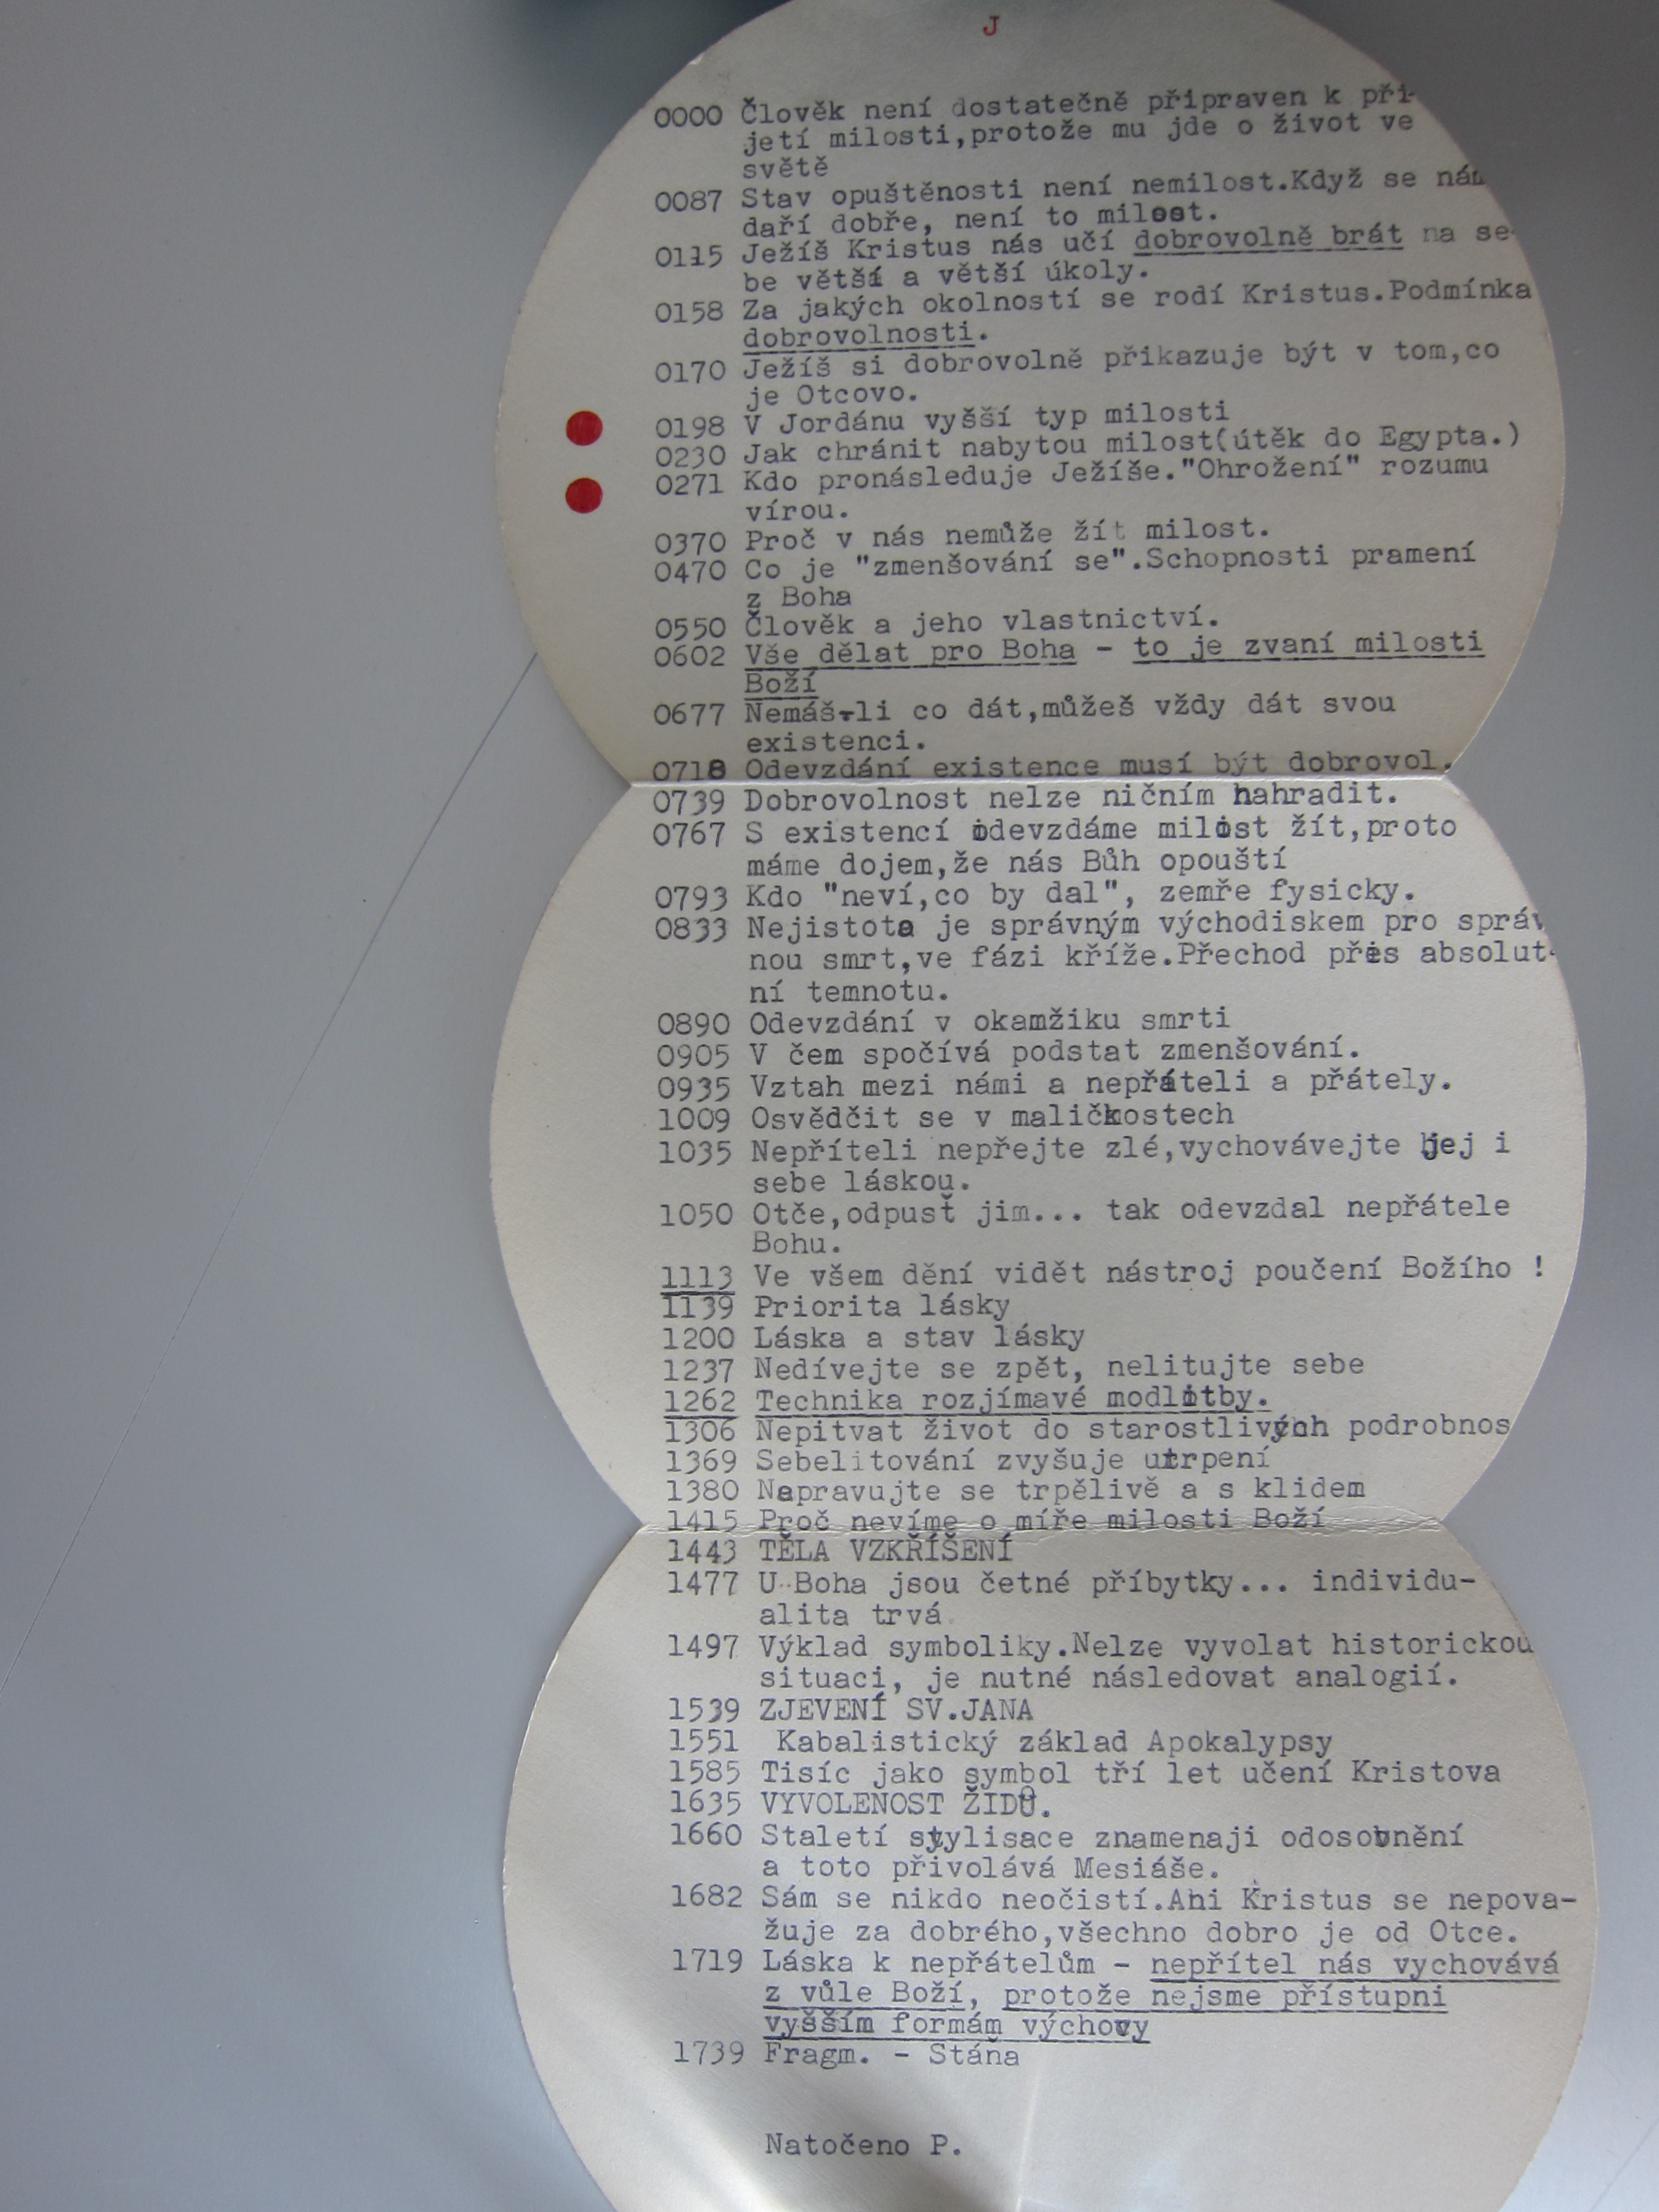
\includegraphics[scale=0.192]{rc/index-kotouc.jpg}
\caption{Index přiložený k~jednomu z~kotoučů.}
\label{fig:index-kotouc}
\end{figure}

Krom toho existují podrobnější indexy ve formě listů
formátu A4, psané z~menší části na stroji, z~větší části psacím písmem, kde
interval mezi jednotlivými úseky je často v řádu desítek sekund. Těch je
nafocených 350 stran. Viz příklad na obrázku~\ref{fig:index-rucni}.

\begin{figure}[htpb]
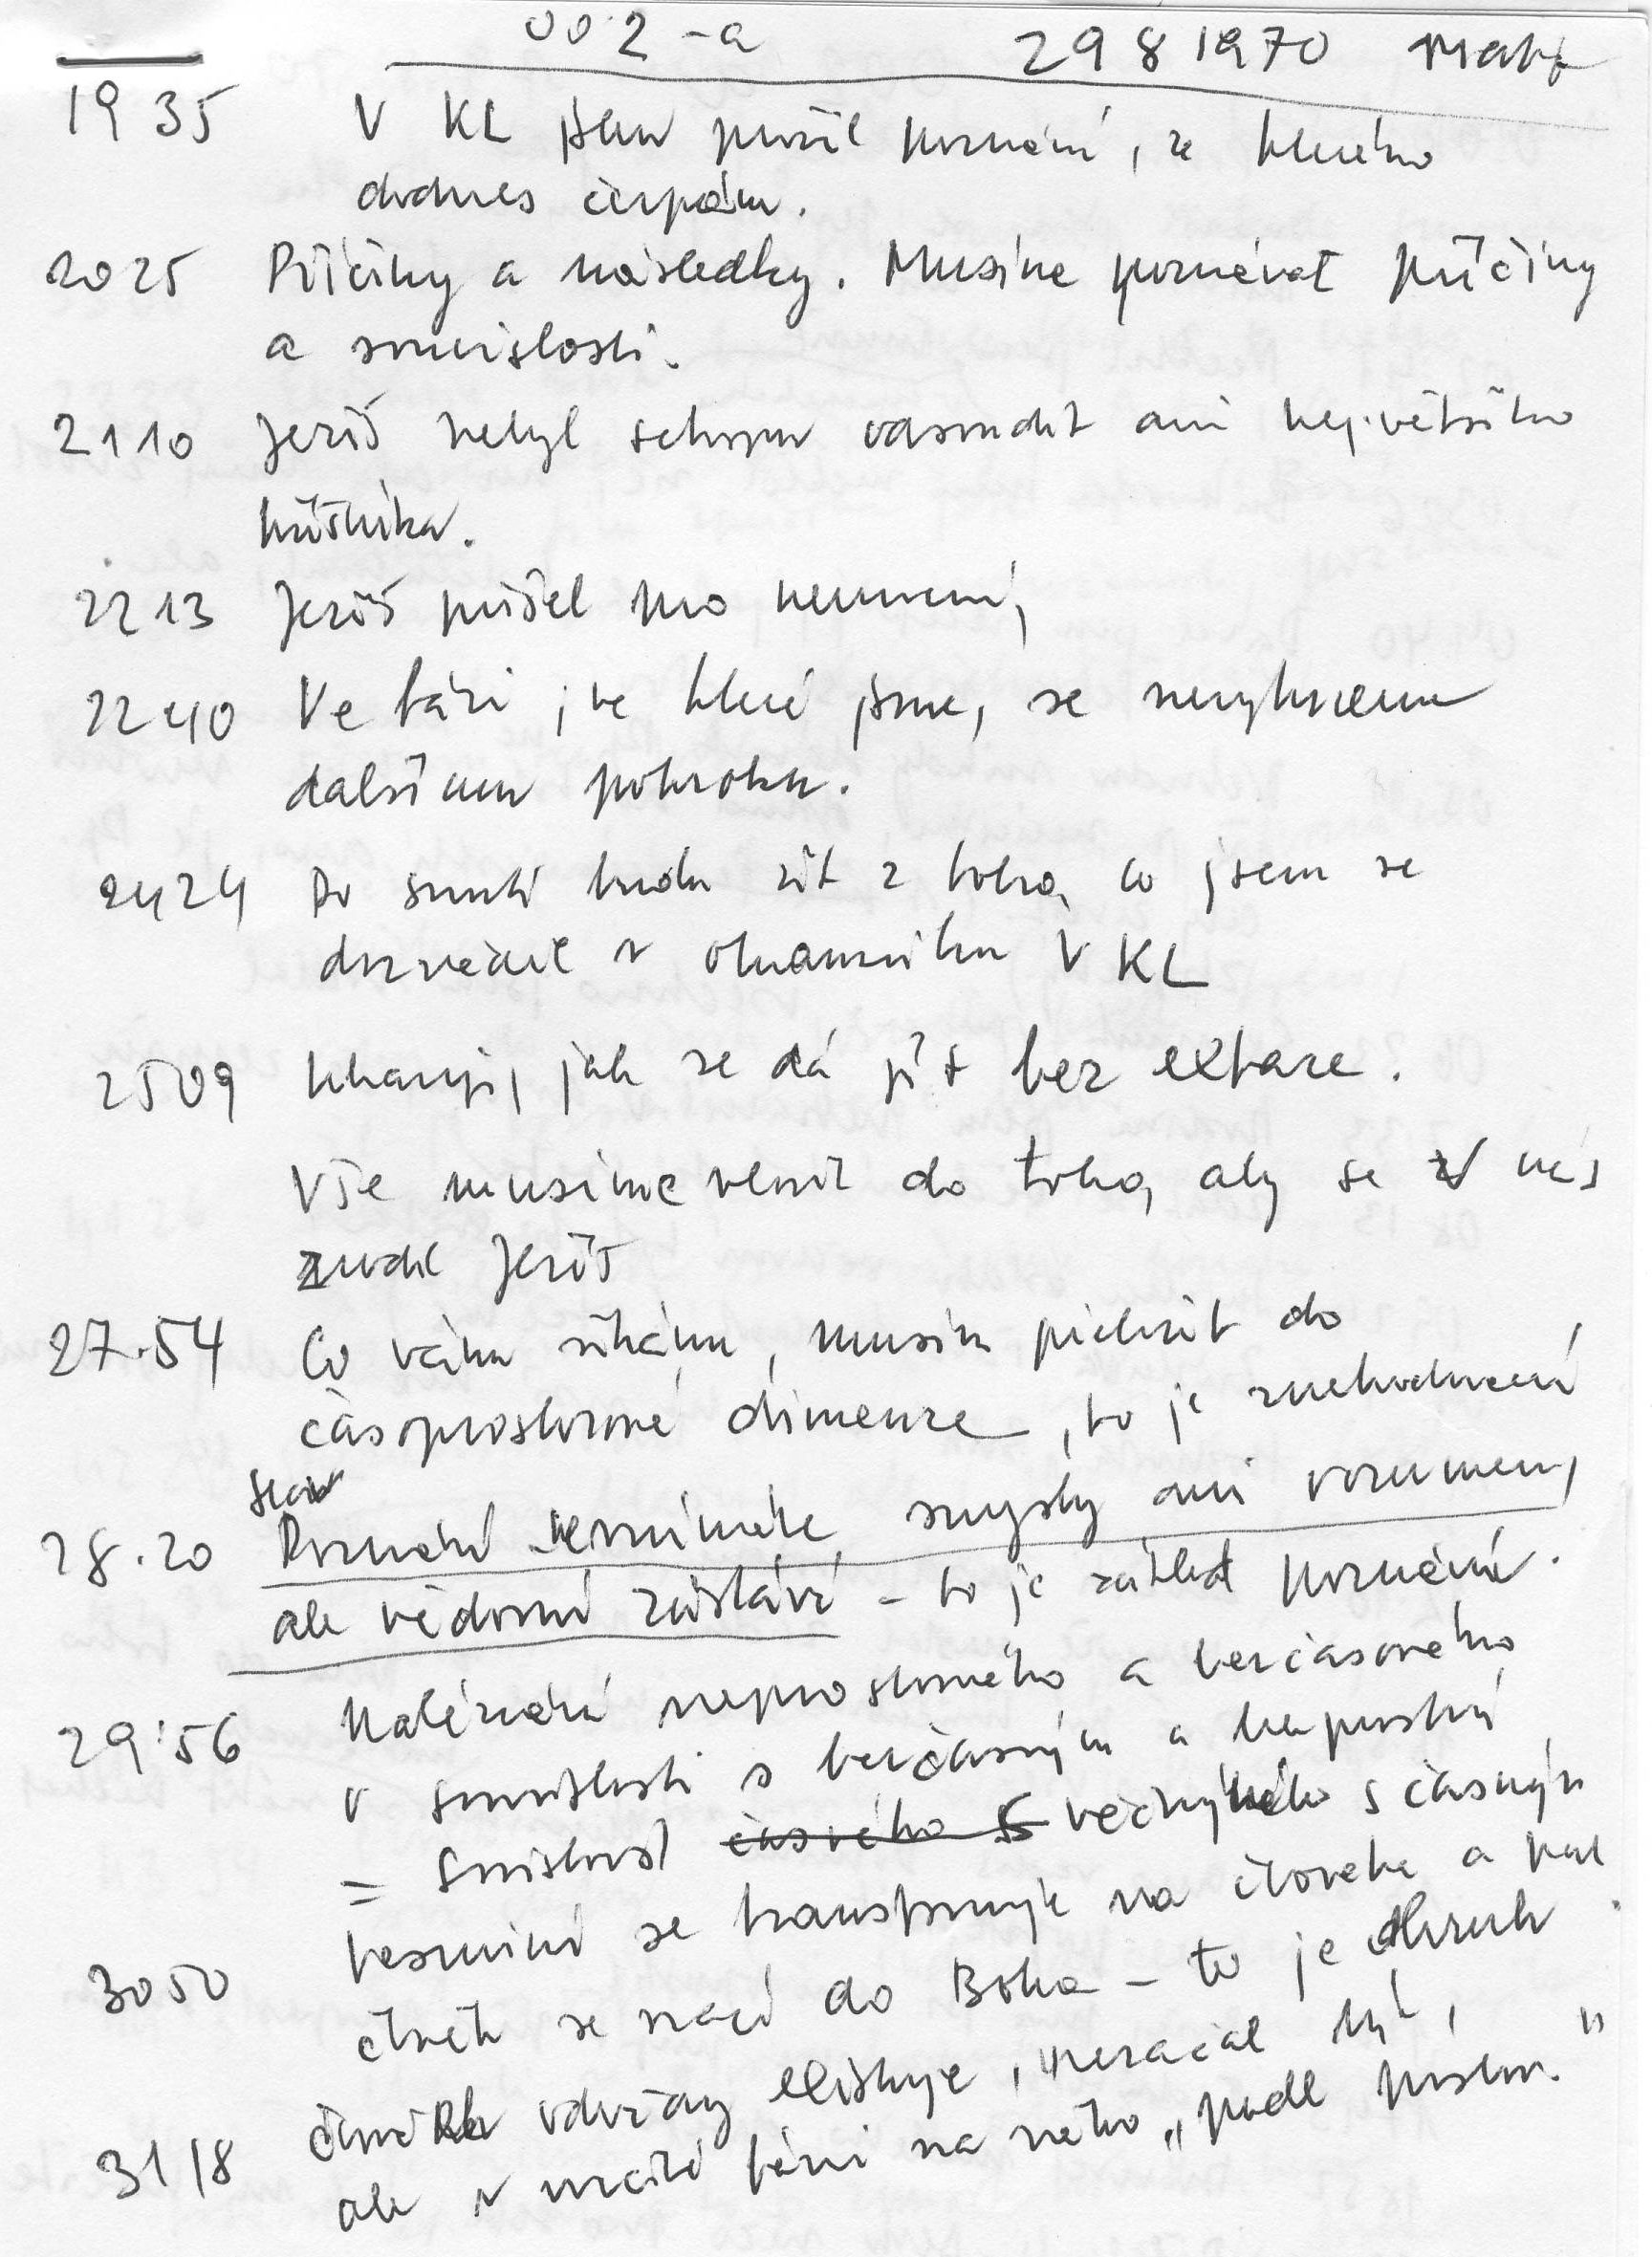
\includegraphics[scale=1.0]{rc/index-rucni.jpg}
\caption{Ručně psaný index.}
\label{fig:index-rucni}
\end{figure}

V~rámci tohoto projektu učinil Ing. Milan Tulach vždy po přepisu přednášky výběr
pasáží, které považoval za stěžejní, a opatřil je časovými značkami.
Pokryl tak toho času 44 nahrávky.

K~poslouchaným nahrávkám si dělám poznámky stejným způsobem jako v~ručně psaných
indexech, jen digitálně a pozice označuji identifikátorem
nahrávky a časovou pozicí. Zatím jsem takto pořídil 2626 záznamů ze~170 nahrávek.

Pozice počítadla magnetofonu v indexech
jsem se pokusil převést na časové údaje. Počítadlo se inkrementuje při každé
otáčce cívky, na kterou se páska navíjí. Uplynulý čas je tedy kvadratická funkce
pozice počítadla. Mělo by tedy stačit nalézt několik málo odpovídajících párů
pozic počítadla a času a z~toho interpolovat koeficienty v~hledaném polynomu.

Tak jsem dospěl k~výrazu $t = 0,0008605c^2 + 1,674c + 3,998$. Bohužel vyšlo
najevo, že po hodině trvání nahrávky se kotouč otáčí tak pomalu, že pozice
počítadla se změní až za několik desítek sekund. To způsobuje, že interpolační
koeficienty jsou velmi nepřesné a v~kombinaci s~nepřesností při určování nové
pozice to způsobuje, že začátek hledaného tématu se nachází i více než minutu
před či za predikovanou pozicí.

Tento problém lze řešit buď přesnějším určením funkce času podle pozice
počítadla, a to použitím hardwarového počítadla či přesnější interpolací
pomocí většího množství bodů, anebo využitím predikce začátku
tématu v~několikaminutovém okolí pomocí komputačnělingvistických metod.

\section{Nahrávání}
\label{sec:data:rec}

O průběhu nahrávání mám pouze kusé a anekdotické informace. Nejstarší datum, na
které jsem u nahrávky narazil, je z~roku 1970. Je možné, že některé nahrávky
jsou staršího data, ale nic nenasvědčuje tomu, že by jich bylo mnoho a byly
výrazně starší. Vzhledem k~tomu, že Karel Makoň začal evangelizovat už
v~koncentračním táboře na konci roku 1939 a přestal až v~roce 1992, je
pravděpodobné, že záznam je k~méně než polovině slov, která vyřkl.

Přednášky v~úzkém kruhu přátel se konaly na různých místech Československa,
později ČR.
Existovala skupinka v~Plzni, v~Praze a v~Gottwaldově, dnešním
Zlíně. Některé z~nahrávek jsou
z~několikadenních skupinových setkání v Kalech u Brna, na chatě Čeřínek v
Českomoravské vrchovině nebo ve Žiaru na Slovensku. Ostatní pocházejí většinou
z~přátelských setkání u někoho v soukromí.

Naprostou většinu nahrávek, které mám k~dispozici, pořídil dr. Elger.
Nahrávalo se s~tehdejší nejmodernější technikou a pásky byly pečlivě
skladovány. Nahrávky z~ostatních míst
také existují, ale jsou spíše raritou a často jsou hůře zachované a ne tak
systematicky označené.

Část nahrávek (30\% celkové délky) je nahraných na kotouče, zbytek na kazety. Ve
většině případů má každý kotouč a každá kazeta identifikátor. Některé kusy
jsou bez identifikátoru, některé dvojice mají totožný identifikátor a různý
obsah.

Většina nahrávek je z~kazet s~identifikátorem ve formátu \texttt{YY-NN}.
Například \texttt{85-05} je pátá kazeta z~roku 1985. Z~takto označených kazet
pochází 686 výsledných souborů z celkových 802, které mají původ v~kazetách.

Celkem z~39 kotoučů, které jsem sám digitalizoval, jich 36 bylo nahraných
rychlostí 9,53 centimetru za sekundu. Zbylé tři rychlostí 2,38 centimetru za sekundu. Na jeden
průchod takového kotouče se vejde šest hodin záznamu, ale za cenu citelného
snížení kvality, zvláště po dekádách skladování. 24 kotouče jsou označeny
písmenem. Posloupnost je více méně abecední, ačkoliv tři různé kotouče sdílejí
identifikátor s~písmenem ,,I`` a nedostala se ke mně žádná páska s~písmenem
,,G``; asi se ztratila. 85 kotoučů (včetně těch, které jsem nedigitalizoval já)
má v~identifikátoru ročník v~rozmezí od 1973 do 1988. Vyskytuje se zde však
mnoho duplicit, takže skutečný počet rozličných nahrávek je v~této kategorii
pravděpodobně mnohem menší. Deset kotoučů má číselný identifikátor, dvacet devět
textový a dva byly vůbec bez identifikátoru.

Existují také dva videozáznamy. Jeden, tříhodinový, je ke zhlédnutí na YouTube:
\texttt{https://www.youtube.com/watch?v=UaNm9jnnJiA}

\section{Digitalizace}
\label{sec:data:digitisation}

U většiny kazet byla digitalizace prováděna stylem jedna strana do jednoho
souboru. U kotoučů to byl jeden kanál jednoho průchodu z~kotouče na kotouč do
jednoho souboru. Výjimku zde tvoří kazety digitalizované v~módu auto-reverse,
s~čímž jsem v~průběhu dvou let digitalizace experimentoval.

Následuje vyčerpávající výčet médií, které odpovídají jednotlivým
digitalizovaným souborům:

\begin{itemize}
\item{strany kazet: 615 souborů,}
\item{celé kazety: 140 souborů,}
\item{průchody z~kotouče na kotouč: 112 souborů,}
\item{převzaté, nejisté: 222 soubory,}
\item{dvě po sobě jdoucí kazety: 1 soubor.}
\end{itemize}

Převzaté soubory byly digitalizovány dříve, než jsem se k~nim dostal. Formát pro digitalizaci, který jsem používal, byl
nejdříve 44100Hz pro prvních 810 souborů, posléze 48kHz,
16 bitů v~reálném čase. Výjimku z~digitalizace v~reálném čase tvoří
kotouče nahrané rychlostí 2,38 cm/s. Ty byly digitalizovány standardní
rychlostí 9,53 cm/s, načež jim byla nastavena čtvrtinová vzorkovací
frekvence.

Pro digitalizaci jsem používal nejdříve zařízení {\em Ion Tape 2 PC}, které
poskytuje USB rozhraní jako externí zvuková karta. Později jsem začal používat
přehrávač {\em Denon DRW-585} a externí zvukovou kartu {\em Lexicon Alpha} coby převodník
z~analogového signálu do digitálního formátu. Kotouče jsem digitalizoval pomocí
přehrávače {\em Tesla B-115} připojeného zezačátku do {\em Ion Tape 2 PC},
později do {\em Lexicon Alpha}.

\subsection{Volba identifikátorů}

Každý takto zdigitalizovaný soubor jsem pojmenoval podle následujícího
algoritmu: Pokud šlo o kazetu s~identifikátorem, použil jsem tento identifikátor
a k~němu připojil písmeno \texttt{A} nebo \texttt{B} pro rozlišení strany. Pokud
byl na obalu nějaký další popisek, připojil jsem ho za pomlčku k~oběma stranám.
Pokud byl popisek na kazetě, připojil jsem ho pouze k~souboru odpovídající strany.

V~případě
kotoučů jsem identifikátor prefigoval řetězcem \texttt{kotouc-} a připojil
rozlišovací dvoumístné číslo počínaje \texttt{01} a označení stopy \texttt{-a}
až \texttt{-d}.

Písmeno \texttt{a} dostal vždy levý kanál prvního průchodu, \texttt{c} pravý
kanál. Písmeno \texttt{b} dostal levý kanál zpátečního průchodu a \texttt{d}
pravý kanál. Ukazuje se, že toto značení nebylo nejšťastněji zvolené, protože
některé kotouče jsem dostal převinuté na opačnou stranu, takže dochází
k~nepředvídatelné záměně mezi písmeny \texttt{a}, \texttt{c} versus \texttt{b},
\texttt{d}.

Pokud nahrávka identifikátor neměla, použil jsem řetězec \texttt{neident} a
pořadové číslo.

\subsection{Přepisy}

K~6. květnu 2020 existuje ke korpusu kompletní přepis o 7 510 610
slovech, z~nichž 715 285, tedy 9,52\% je přepsáno ručně.
Ruční přepisy pokrývají přesně 107 hodin 41 minutu a 49 sekund z~celkových
1050 hodin 5 minut a 3 sekund nahrávek.

První manuálně přepsaný segment byl pořízen v~dubnu 2012 a od té doby do dneška
jich bylo posláno 128 038. Z~toho 113 846, to jest 89\%, pochází od čtyř
přispěvatelů (mezi něž já nepatřím).
Obrázek~\ref{fig:corpus-growth} ukazuje, jak přibývaly hodiny přepisů v~čase.
Počítá se zde celkový objem příspěvků, které se namnoze překrývají, takže
skutečný čas přepsaného záznamu je ,,jen`` zmiňovaných 107 hodin.

\begin{figure}[htpb]
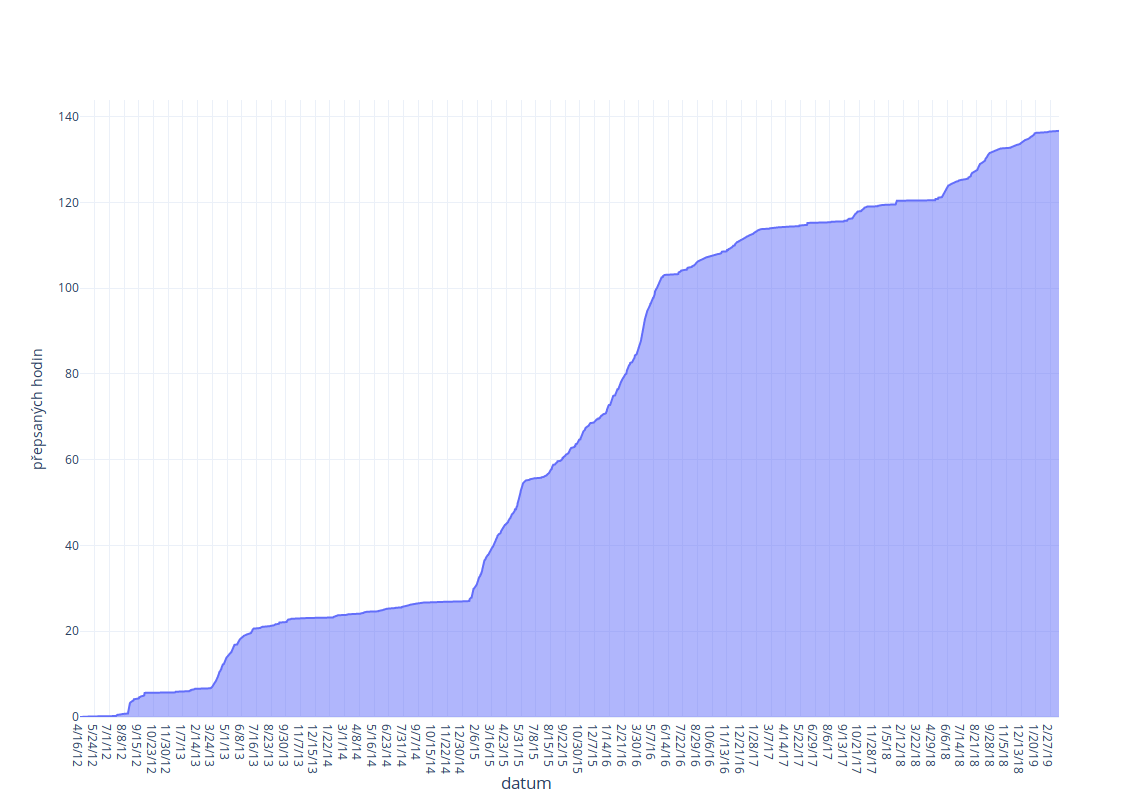
\includegraphics[scale=0.39]{rc/corpus-growth.png}
\caption{Přibývání celkového času oprav.}
\label{fig:corpus-growth}
\end{figure}

Podíl manuálně a automaticky přepsaných pasáží ilustruje
obrázek~\ref{fig:humbits}. Každý pixel reprezentuje jedno slovo v~přepisu,
přičemž černé pixely představují manuálně přepsaná slova.

\begin{figure}[htpb]
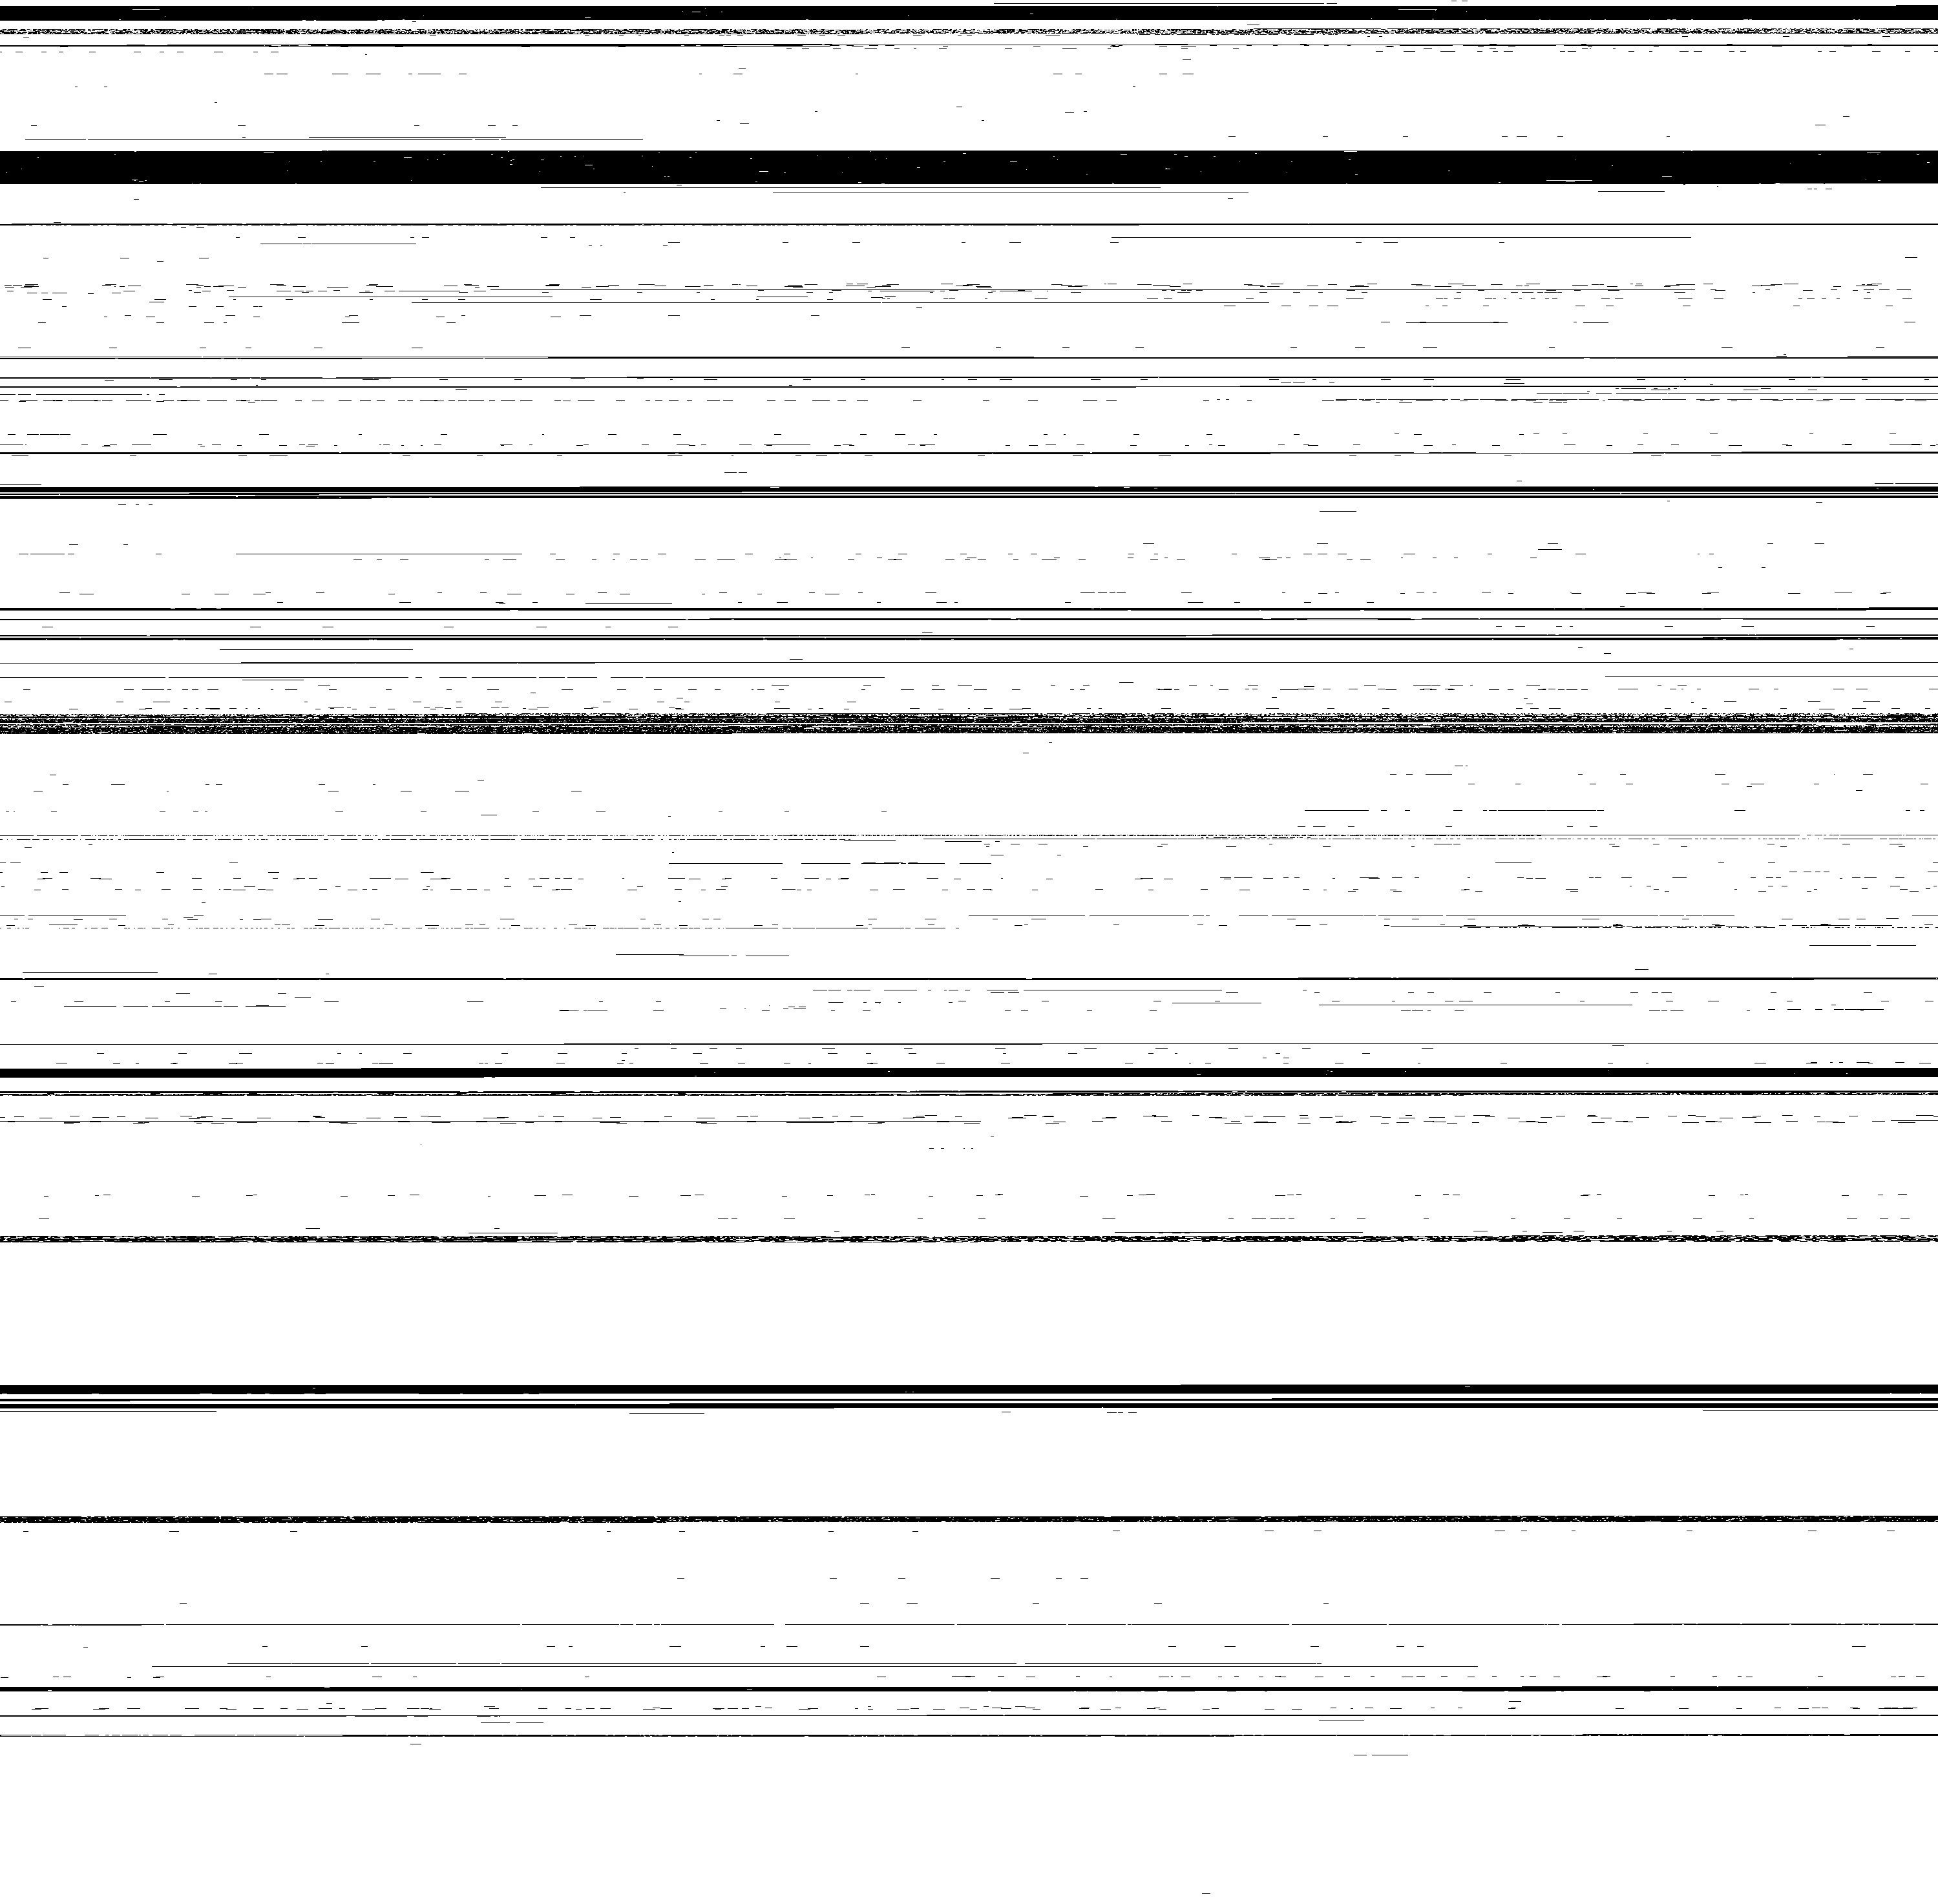
\includegraphics[scale=0.137]{rc/humbits.png}
\caption{Distribuce automaticky (bílá) a manuálně (černá) pořízených přepisů.}
\label{fig:humbits}
\end{figure}

Mechanismus pořizování přepisů dopodrobna rozvádí kapitola~\ref{kap:webove-rozhrani}. 

\chapter{Akustické vlastnosti Makoňova korpusu}
\label{kap:akustika}

Mluvený korpus Karla Makoně vyniká vzhledem ke své velikosti konzistencí téměř
výlučně jediného mluvčího a velmi úzkou tematickou doménou. Jistou protiváhu
této konsistentnosti představují jeho akustické vlastnosti.

\section{Výchozí akustická kvalita}

Akustická kvalita nahrávek je největší slabinou korpusu. Kvalita není
konzistentně špatná, je velmi kolísavá. Na kvalitu záznamu má vliv jeho stáří,
použité médium, rychlost záznamu, způsob skladování, zda se jedná o
originál\footnote{kopírování magnetofonových pásek je ztrátový proces}, použitý
magnetofon, mikrofon, pozice mikrofonu, akustické vlastnosti prostředí jako
ozvěna, hluk na pozadí, ale také momentální dispozice mluvčího.

Obrázky~\ref{fig:spectr-ok} až~\ref{fig:spectr-fasttalk} ukazují spektrogramy
nahrávek různých kvalit. Vždy se jedná přibližně o třísekundový úsek a součástí
popisku je odkaz pro přehrání odpovídajícího zvuku.

\begin{figure}[htpb]
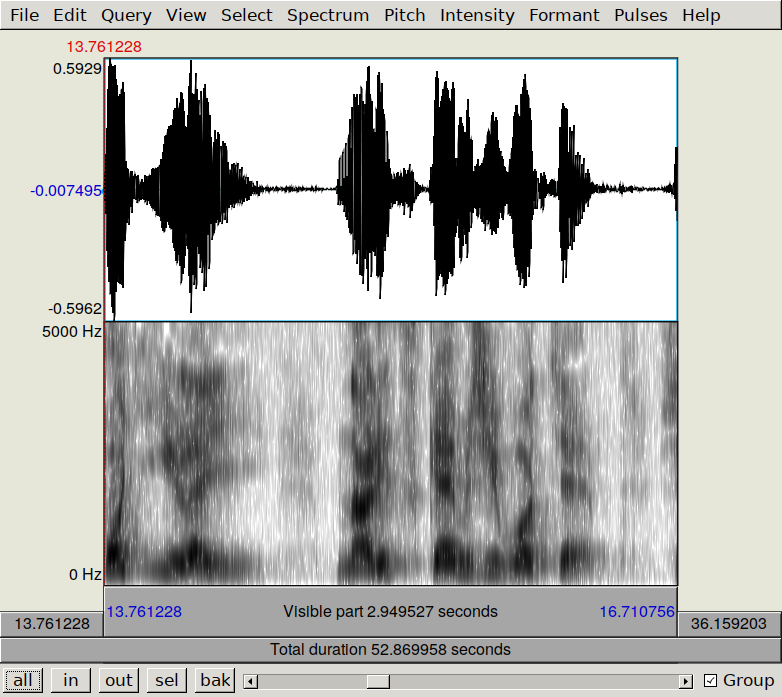
\includegraphics[scale=0.89]{rc/spectrum-dobry-90-02A.png}
\caption{
    kvalitní záznam bez zjevných defektů\\
    \texttt{http://radio.makon.cz/zaznam/90-02A\#ts=673.14}
}
\label{fig:spectr-ok}
\end{figure}

\begin{figure}[htpb]
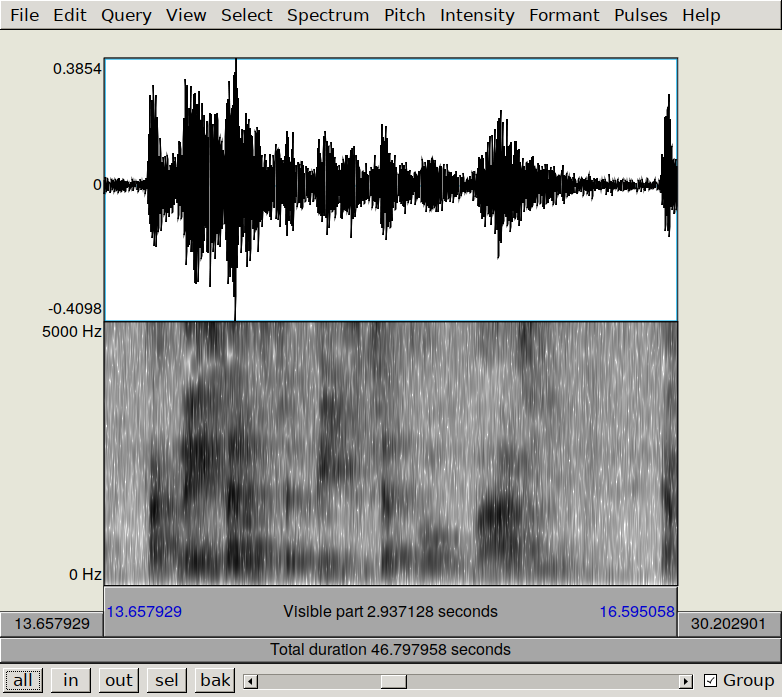
\includegraphics[scale=0.89]{rc/spectrum-echo-90-24A.png}
\caption{
    výrazné echo\\
    \texttt{http://radio.makon.cz/zaznam/90-24A-24.4.90\#ts=664.33}
}
\label{fig:spectr-echo}
\end{figure}

\begin{figure}[htpb]
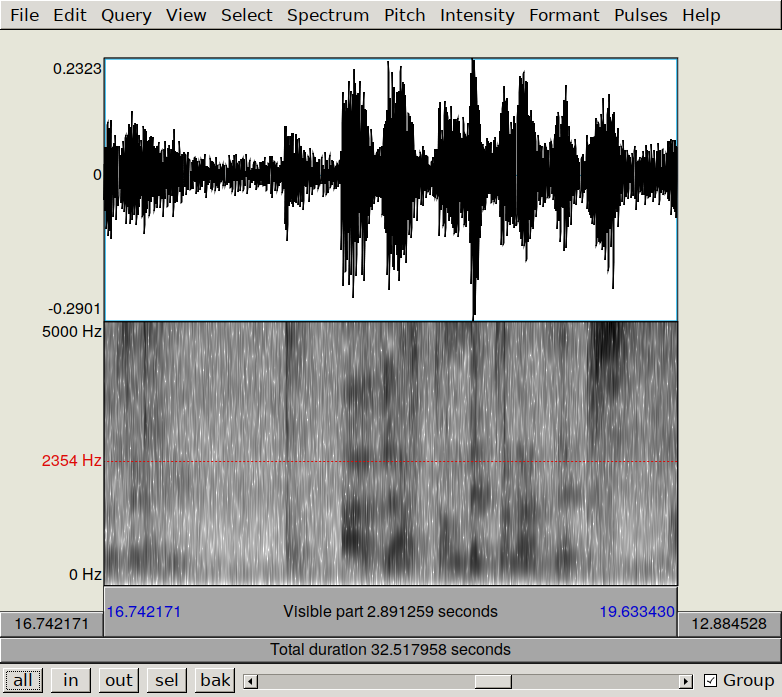
\includegraphics[scale=0.89]{rc/spectrum-noise-92-04A.png}
\caption{
    širokopásmový šum\\
    \texttt{http://radio.makon.cz/zaznam/92-04A\#ts=691.37}
}
\label{fig:spectr-noise}
\end{figure}

\begin{figure}[htpb]
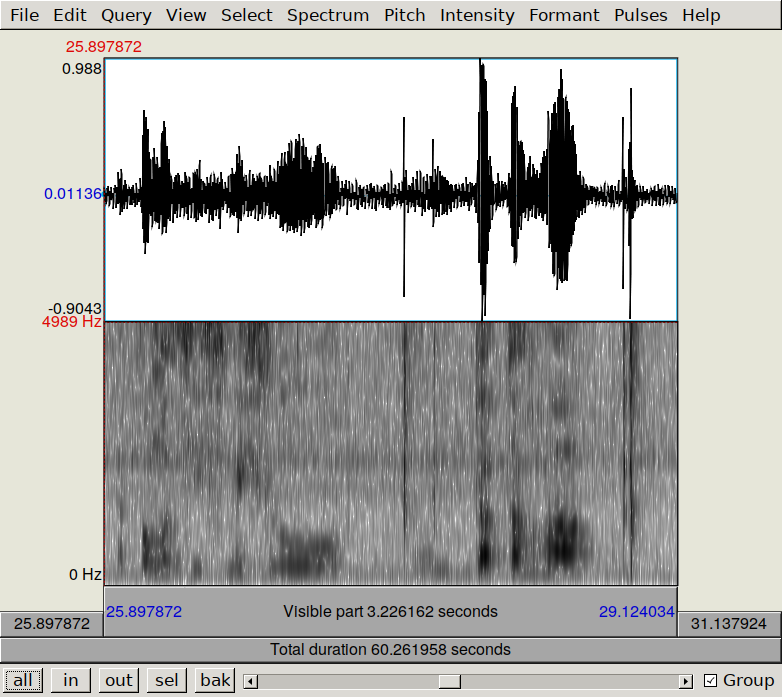
\includegraphics[scale=0.89]{rc/spectrum-narrow-92-03B.png}
\caption{
    úzkopásmový šum\\
    \texttt{http://radio.makon.cz/zaznam/92-03B\#ts=664.43}
}
\label{fig:spectr-narrow}
\end{figure}

\begin{figure}[htpb]
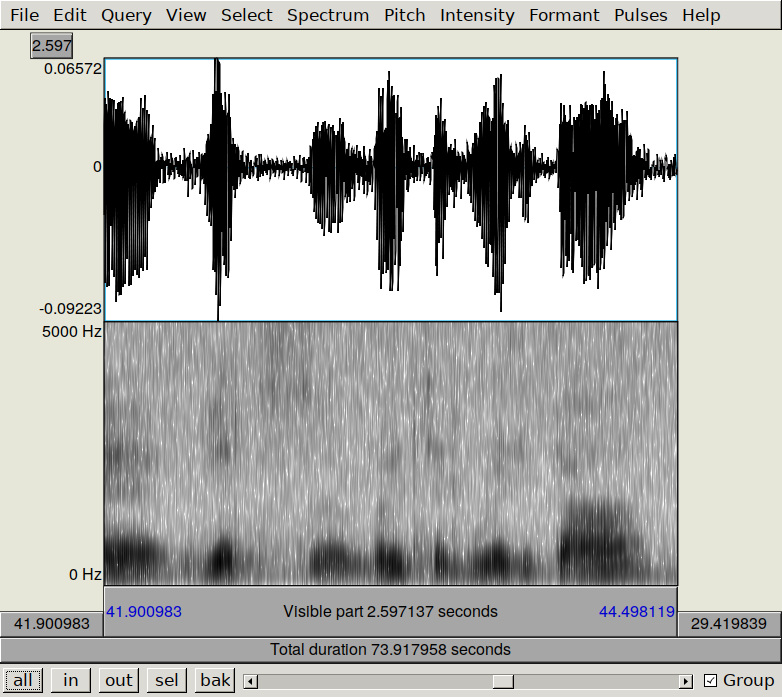
\includegraphics[scale=0.89]{rc/spectrum-nohighs-88-04A.png}
\caption{
    absence vysokých frekvencí\\
    \texttt{http://radio.makon.cz/zaznam/88-04A\#ts=678.94}
}
\label{fig:spectr-nohi}
\end{figure}

%\begin{figure}[htpb]
%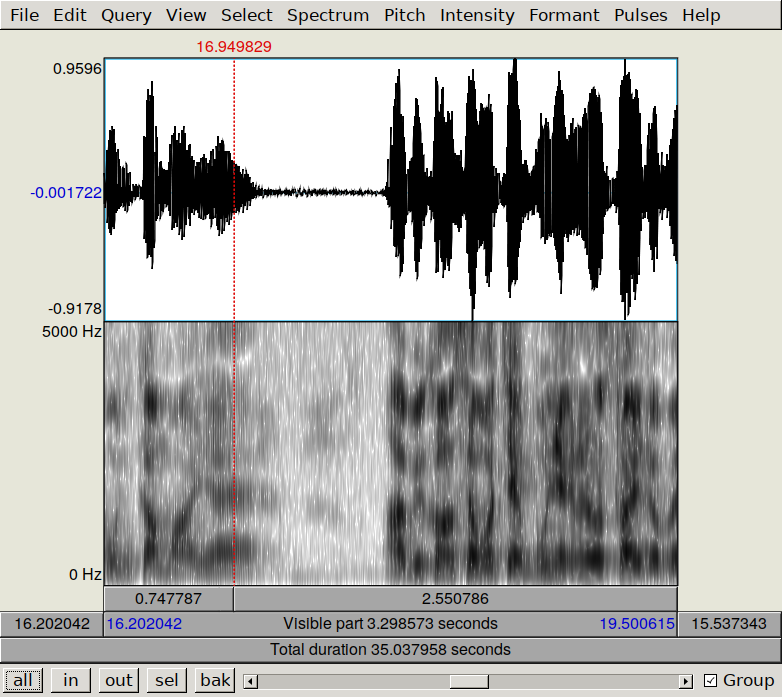
\includegraphics[scale=0.89]{rc/spectrum-overdrive-91-20A.png}
%\caption{
%    přebuzení
%    \texttt{http://radio.makon.cz/zaznam/91-20A\#ts=600.00}
%}
%\label{fig:spectr-overdrive}
%\end{figure}

\begin{figure}[htpb]
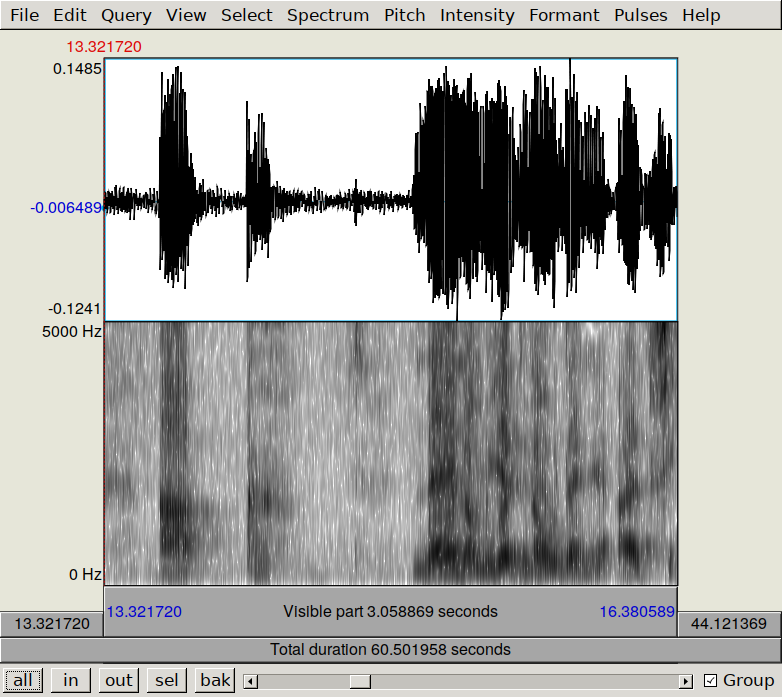
\includegraphics[scale=0.89]{rc/spectrum-accel-90-18A.png}
\caption{
    zrychlený záznam způsobený zpomalením převíjení pásky při nahrávání\\
    \texttt{http://radio.makon.cz/zaznam/90-18A-XX-zrychlene\#ts=2473.56}
}
\label{fig:spectr-accel}
\end{figure}

\begin{figure}[htpb]
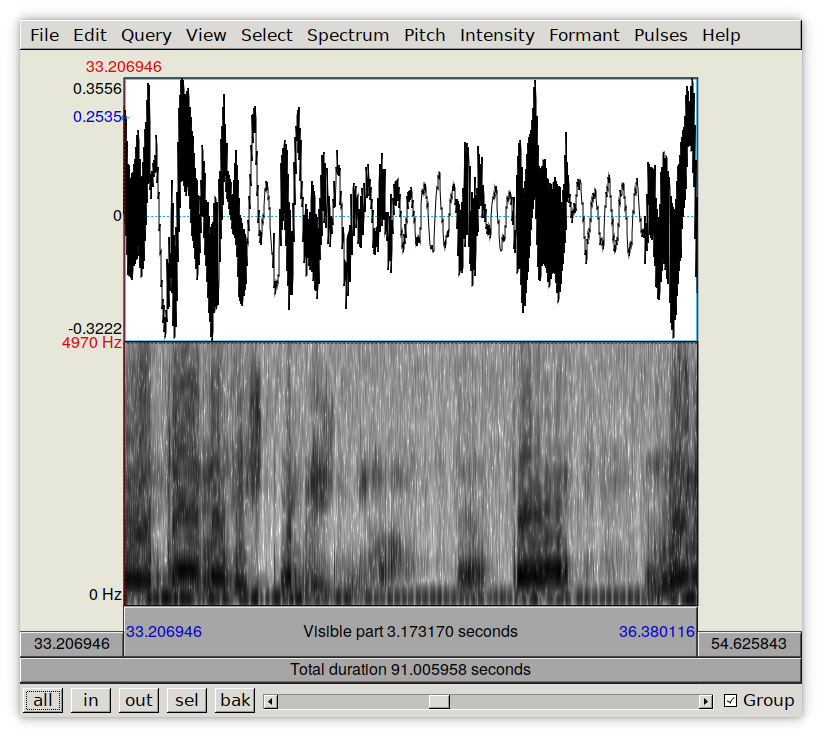
\includegraphics[scale=0.89]{rc/spectrum-2cms-ktplzneid01a.png}
\caption{
    silně degradovaná nahrávka pořízená rychlostí 2,38 cm/s\\
    \texttt{http://radio.makon.cz/zaznam/kotouc-plzen-neident01-a\#ts=660}
}
\label{fig:spectr-2cms}
\end{figure}

\begin{figure}[htpb]
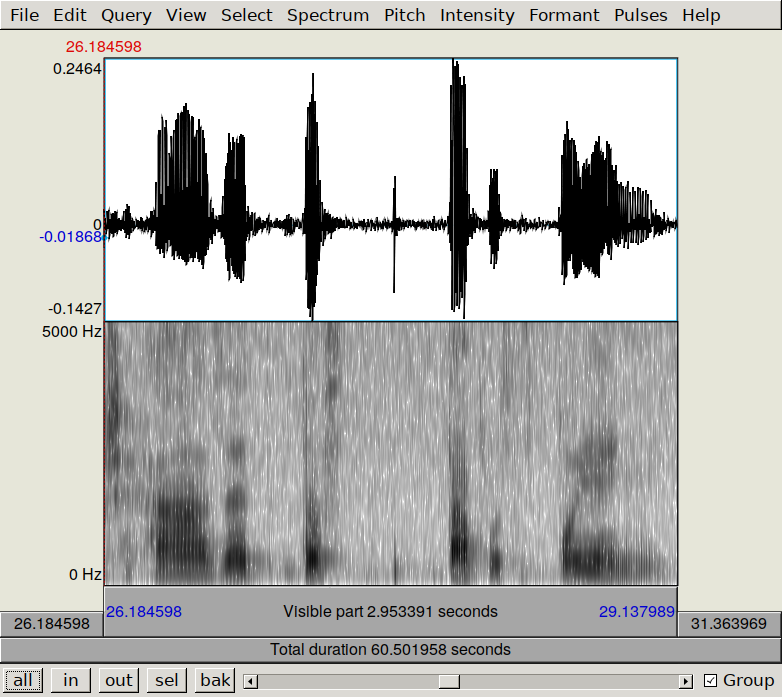
\includegraphics[scale=0.89]{rc/spectrum-pomala-mluva-76-04A.png}
\caption{
    pomalá mluva\\
    \texttt{http://radio.makon.cz/zaznam/76-04A-Kaly-7-IEOUA\#ts=13.79}
}
\label{fig:spectr-slowtalk}
\end{figure}

\begin{figure}[htpb]
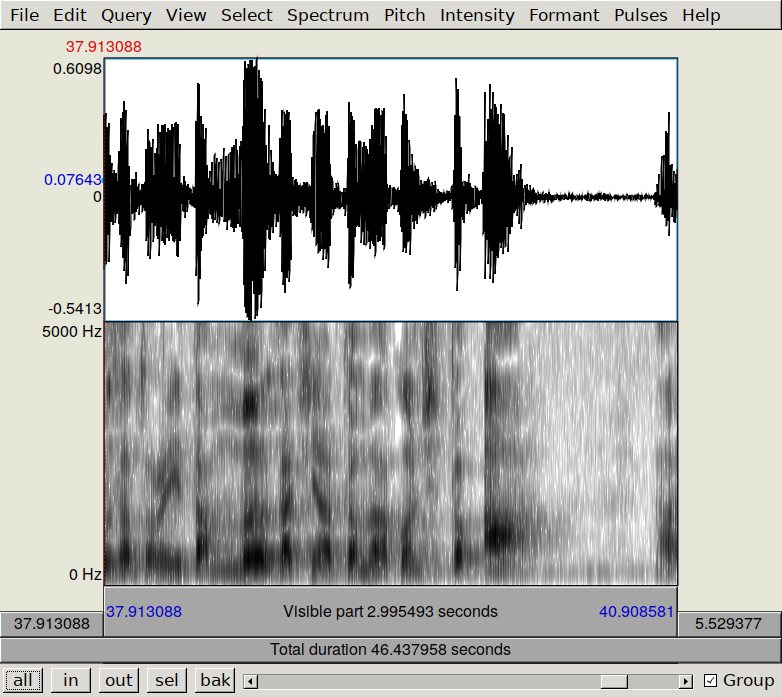
\includegraphics[scale=0.89]{rc/spectrum-rychla-mluva-89-11B.png}
\caption{
    rychlá mluva\\
    \texttt{http://radio.makon.cz/zaznam/89-11B\#ts=203.17}
}
\label{fig:spectr-fasttalk}
\end{figure}

Systematicky můžeme rušivý signál rozdělit takto:
\begin{enumerate}
\item{
    aditivní šum, jevící se jako hučení až syčení a obzvlášť patrný v~tichých
    pasážích,
}
\item{
    stacionární nebo téměř stacionární rušení, například monotónní pískání na
    několika frekvencích, které produkuji nekvalitní obvody magnetofonu
    nebo mazací tón,
}
\item{
    nestacionární rušení, např. řeč na pozadí, bouchnutí dveří apod.,
}
\item{
    velká ozvěna místnosti nebo špatně ekvalizovaný mikrofon zesilující
    některé frekvence na úkor jiných,
}
\item{
    nelineární zkreslení magnetofonu,
}
\item{
    kolísání rychlosti.
}
\end{enumerate}
Ty nastávají při záznamu na magnetofonový pásek. Při přehrávání dochází
k~dalším.

\section{Metrika}
\label{sec:akustika:metrika}

Předpokladem pro práci s~akustickými vlastnostmi dat je porovnávání na jejich
základě. Je tedy nutné mít metriku, která by odrážela akustickou podobnost
jednotlivých souborů. K~tomu využívám algoritmu založeného na koeficientech
MFCC, jak to navrhují Mandel a Ellis\cite{mandel2005song}. Využívám
k~tomu programu Musly od Dominka Schnitzera\cite{schnitzer2011using}.

V~rámci nahrávek dochází často ke změnám akustických vlastností. To je dáno
hlavně tím, že se nahrávání uprostřed pásky přerušilo a obnovilo se v~jiných
podmínkách. Není proto žádoucí porovnávat celé nahrávky. Ideální by bylo
detekovat akustické zlomy v~nahrávkách a korpus přerozdělit ne podle hranic
nahrávek, ale podle těchto zlomů.

Pro jednoduchost jsem nahrávky rozdělil do menších úseků a udělal matici
akustické vzdálenosti na nich. Pokusil jsem se využít hotových úseků rozdělených
v~bodech ticha, viz sekci~\ref{sec:segmenty}. Výsledná matice o rozměrech
80~000 × 80~000 však trpěla defekty při čtení a zápisu, proto jsem velikost
úseků pro tento účel zvětšil na 10 minut a tím dosáhl počtu 8146 úseků.

Pro orientaci uvedu některé údaje z~matice podobnosti. 
Medián vzdálenosti je 55,8.
Maximální vzdálenost je $3,40\cdot{}10^{38}$, ovšem ta nastává v~okrajových
případech, bez zjevného důvodu patrného lidskému uchu. Bez této astronomické
maximální vzdálenosti dosahují vzdálenosti hodnot do 27~814.
Počet nulových vzdáleností je 275 z~celkových 33~174~585.



Abychom tato čísla mohli interpretovat, porovnejme je se vzdálenostmi jiných
zvuků, které si snad čtenář dokáže představit.

Ku příkladu tři různí mluvčí jednoho záznamu jednání poslanecké sněmovny
parlamentu České republiky mají vzdálenost v rozmezí 6,5 a 9,5. Dva různé úseky
téhož mluvčího mají vzdálenost 1,4. Tyto záznamy z PSP ČR jsou i pro lidské ucho
velmi podobné a na rozdílu ve vzdálenosti mezi různými mluvčími a v~rámci
mluvčího je vidět, že algoritmus funguje dobře.

Jako druhý příklad vezměme typickou, úsměvně známou ukázku mluveného slova
s~hlukem na pozadí, a sice úryvek ,,to je dost, žes nás taky jednou vyvez, žes
udělal něco pro rodinu`` z~filmu Slavnosti sněženek. Jednotliví mluvčí (Blažena
Holišová a Rudolf Hrušínský) mají vzájemnou vzdálenost 13,9. Holišová od
samotného malotraktoru 48,2 a Hrušínský od téhož 23,7.

Srovnejme ještě mluvenou řeč s~populární hudbou. Uvedu dva extrémní příklady, na
které jsem narazil:
Skladba Billie Jean od Michalea Jacksona má od poslance Sklenáka vzdálenost
23,1, zatímco refrén skladby Shadow Sun od metalové skupiny Moonspell od
poslance Okamury 519.

Je tedy patrno, že akustická variabilita korpusu Karla Makoně je i podle tohoto
měřítka obrovská.

\section{Shlukování}

Kompenzovat akustické nedostatky znamená měnit akustické kvality dat tak, aby
lépe odpovídaly nějakému kritériu. To může být subjektivní: aby se zvuk určitému
posluchači lépe poslouchal. Může být také objektivní, strojově vyhodnotitelné,
což pak umožní nasazení strojových metod.

V~korpusu Karla Makoně se nevyskytuje asi žádná nahrávka ve vysoké kvalitě
srovnatelné s~materiálem pořízeným ve studiových podmínkách. Velká část
nahrávek, obzvlášť kazety z~let 1984 a dál, jsou veskrze srozumitelné a bez
zásadních defektů. Z~celého korpusu jsem vybral množinu 431 souboru v~uspokojivé
kvalitě.

Tato referenční množina je mnohem konzistentnější co do akustické metriky než
celý korpus, ale v~porovnání s~ilustračními příklady mimo korpus stále řádově
divergentnější. Vzdálenosti se pohybují od 1,6 do 14~653 s~průměrem  54,7 a
mediánem 9,40.

Na množině úseků, které jsem porovnával akustickou metrikou, jsem provedl
hierarchické shlukování. Vzdálenost clusteru jsem nastavil jako maximální
vzdálenost mezi dvěma prvky, aby jednotlivé clustery byly co nejkompaktnější.

\section{Kompenzace}
\label{sec:akustika:kompenzace}

Akustické nedostatky ztěžují rozpoznávání řeči a jsou tak už dlouho předmětem
bádání. Ku příkladu Gillespie a Atlas\cite{gillespie2002diversity} ukazují
zdrcující vliv dozvuku (angl. {\em reverberation}) na rozpoznávání řeči pomocí
markovovských modelů a zkoumají možnosti kompenzace. Jošioka et
al.\cite{reverbmagazine} předkládají souhrn technik pro kompenzaci dozvuku, Ko
et al.\cite{reverbaugment} digitálně simulují dozvuk v~trénovacích datech.
Seltzer et al.\cite{dnnnoiserobust} se věnují tematice šumu v~rozpoznávání řeči
založeném na hlubokých neuronových sítích.

Revoluční článek\cite{cyclegan}, v~němž Žú et al. představují CycleGAN, čili
cyklicky konzistentní generativní oponentní síť, dal lidstvu do rukou mocný
nástroj a zábavnou hračku, která našla využití pro odstraňování mlhy
z~fotografií\cite{Engin_2018_CVPR_Workshops}, udělování cizích grimas
tvářím\cite{jin2017faceoff}, v~biomedicíně\cite{yang2018biogan} a také pro
zpracování mluvené řeči: Kaneko a Temeoka\cite{kaneko2017parallel} předkládají
doménový transfer hlasu a Hoseini-Asl et al.\cite{hosseini2018malevoicegan} činí
totéž pro účely rozpoznávání řeči. Nejblíže mému problému je Pascual et al.
s~projektem SEGAN\cite{pascual2017segan}, kde se GAN používá pro odstranění
šumu.

CycleGAN je stvořena pro použití na dvou sadách dat, z~nichž každá reprezentuje
určitou doménu, mezi nimiž lze najít mapovací funkci. V~případě korpusu Karla
Makoně je jedna jasná doména akusticky relativně dobrých nahrávek a celý zbytek,
který ovšem konzistentní doménu netvoří. Poškozené nahrávky trpí různými
kombinacemi neduhů v~růnzné míře. Nelze proto CycleGAN přímo aplikovat na
,,zdravé`` a ,,poškozené`` nahrávky. Jak by taky bylo lze nalézt funkci mapující
nahrávku bez neduhů na poškozenou, když není jasné, jaké poškození by měla
vykazovat. Tento směr sice není kýžený, ale pro natrénování dané architektury
nezbytný.

Adaptace GAN tak, aby si s~nekonzistentními daty na jedné straně převodu
poradila, by jistě byla zajímavým a přínosným počinem, nicméně začít se dá
využitím výše zmíněného shlukování, které poskytuje potřebné konzistentní
domény poškozených nahrávek.

Experiment jsem provedl na dvou shlucích: 1) na přebuzených nahrávkách a 2) na
nahrávkách pořízených nízkou rychlostí 2,38cm/s. Oba shluky jsem vybral tak, aby
měly maximální interní vzdálenost 25. Pro trénování jsem použil metodu
navrhovanou dvojicí Kaneko a Tameoka\cite{kaneko2017parallel}, jak ji
implementoval Lei Mao\footnote{github.com/leimao/Voice\_Converter\_CycleGAN}.
Tréning běžel po 200 epoch.

\subsection{Vyhodnocení}
\label{sec:akustika:vyhodnoceni}

Tabulka~\ref{tab:ganeval} uvádí WER při automatickém přepisu na tom kterém
shluku původně a po transferu. Toto porovnání bylo provedeno pomocí modelu
natrénovaného pouze na promluvách Karla Makoně. Robustnější model popsaný
v~sekci~\ref{sec:deepspeech} má chybovost na nízkorychlostních nahrávkách
42,1\% %0.421338
a 34,8\%  %0.348183
na nahrávkách přebuzených.

\begin{table}[htpb]
\begin{center}
\begin{tabular}{|l||r|r|}
\hline
                 & původní & po transferu \\
\hline
přebuzené        & 45,0\%   & 44,1\% \\
nízkorychlostní  & 68,5\%   & 93,9\% \\
\hline
\end{tabular}
\caption{chybovost WER u dvou skupin poškozených nahrávek před a po doménovém
transferu}\label{tab:ganeval}
\end{center}
\end{table}

Mírné, ale patrné umenšení chybovosti u přebuzených nahrávek sice samo o sobě
nepřináší kýžené řešení problému s~neuspokojivými výsledky rozpoznávání
poškozených nahrávek, ale poskytuje příslib potenciálu metody. Snad důležitější
než zvýšená úspěšnost automatického přepisu je však zvýšený komfort při
poslechu. Bohužel pro tento přínost zatím nemám kvantitativní vyhodnocení, ale
subjektivně ho potvrdit mohu.

U katastrofálního zvýšení chybovosti po transferu velmi poškozených nahrávek
pořizovaných nízkou rychlostí je nutno se pozastavit.
Obrázek~\ref{fig:gan:plzen} ukazuje, jak se u těchto nahrávek doménový transfer
odrazil v~průběhu signálu a ve spektru. Obrázek~\ref{fig:gan:overdrive} ukazuje
pro porovnání totéž u přebuzených nahrávek. Povšimněme si, jak u nahrávek
pořízených nízkou rychlostí po přesunu zcela zmizela některá slova. Je-li signál
příliš těžko odlišitelný od ruchů, transfer patrně raději změní takový úsek
v~ticho.

\begin{figure}[htpb]
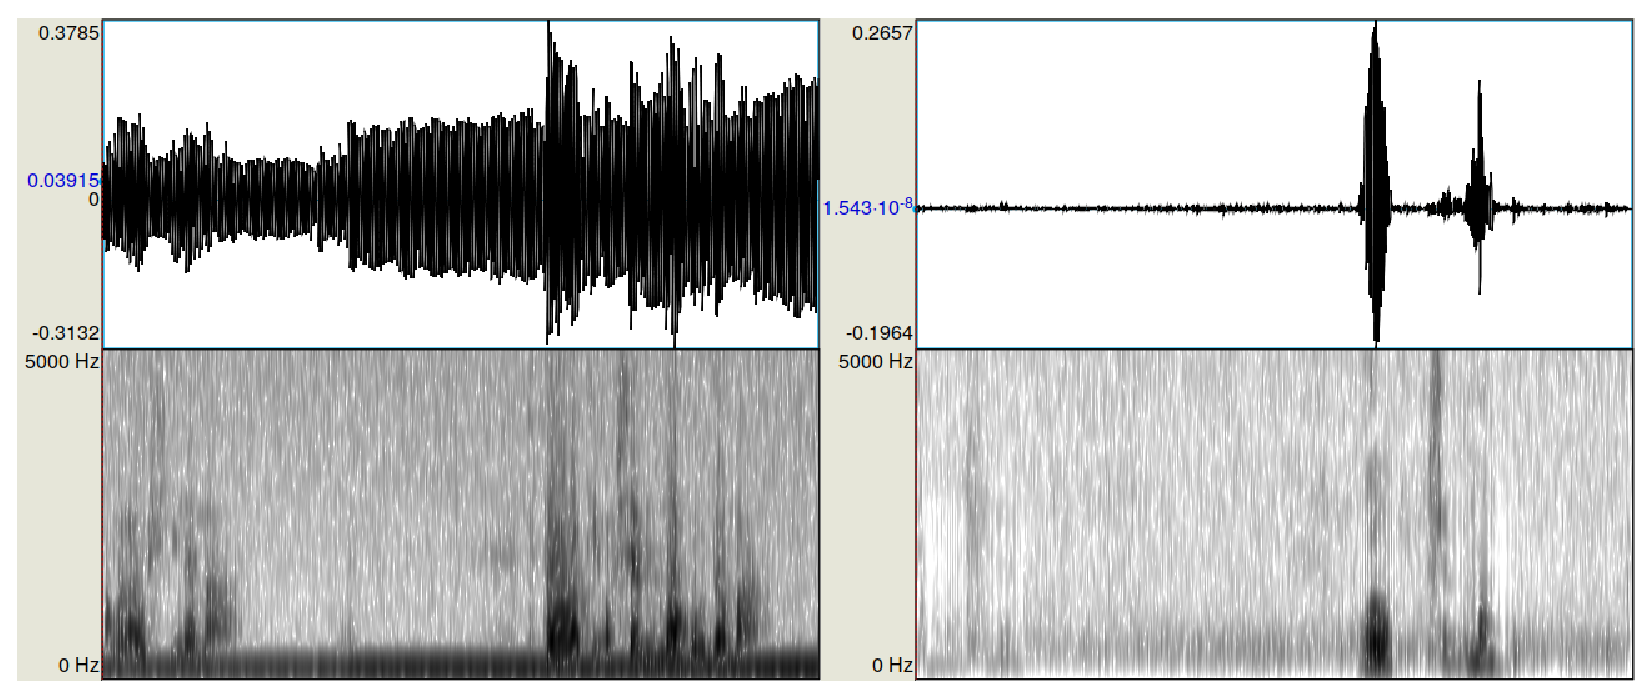
\includegraphics[scale=0.4]{rc/gan-plzen.eps}
\caption{průběh signálu (nahoře) a spektrogram (dole) nahrávky pořízené
rychlostí 2,38cm/s před doménovým transferem (vlevo) a po něm (vpravo)}
\label{fig:gan:plzen}
\end{figure}

\begin{figure}[htpb]
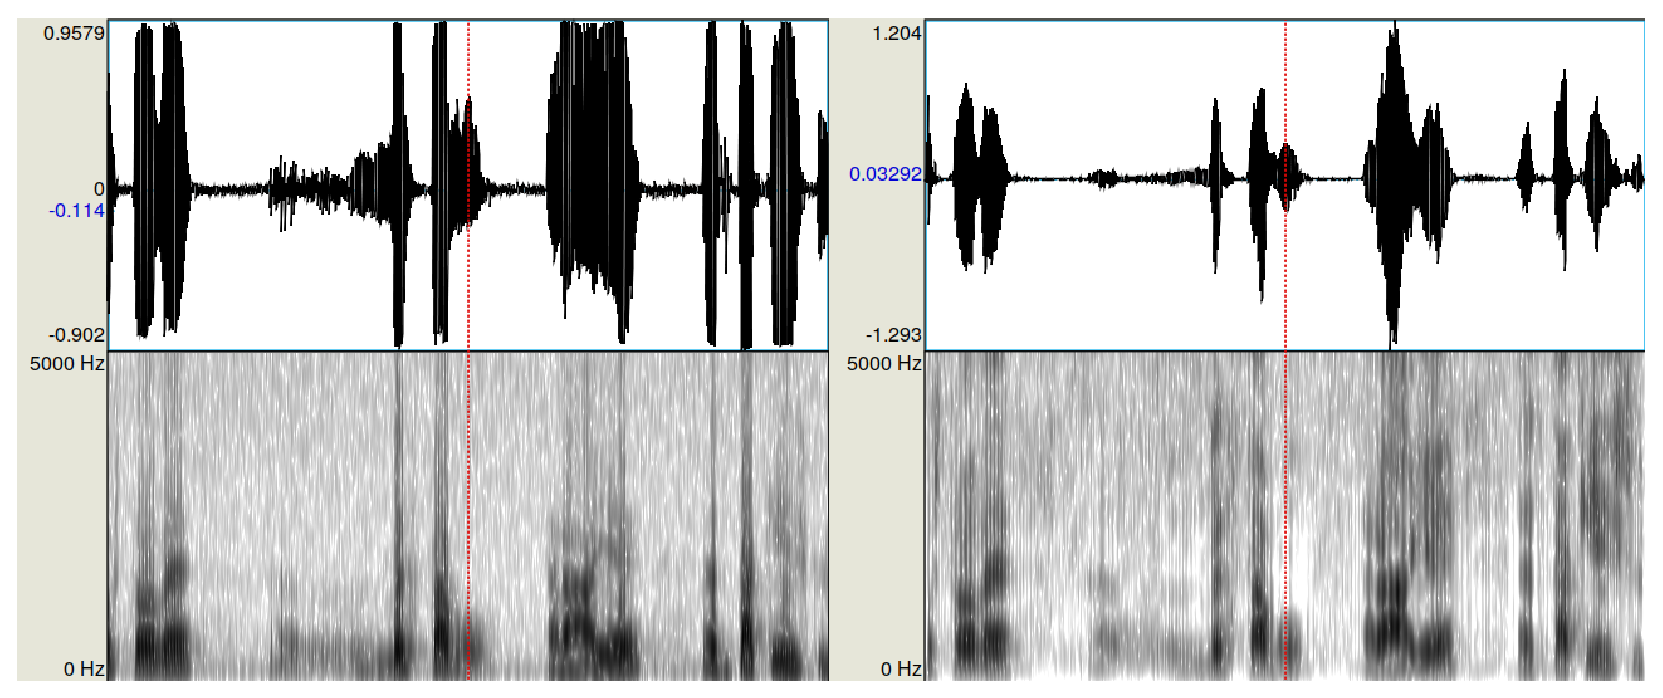
\includegraphics[scale=0.4]{rc/gan-overdrive.eps}
\caption{průběh signálu (nahoře) a spektrogram (dole) přebuzené nahrávky
před doménovým transferem (vlevo) a po něm (vpravo)}
\label{fig:gan:overdrive}
\end{figure}

\chapter{Jednání parlamentu jako trénovací data}
\label{kap:svolocz}

Trénovacích dat pro rozpoznávání řeči není nikdy dost. V~době psaní tohoto textu
je manuálně přepsaných asi 100 hodin z~mluveného korpusu Karla Makoně. To je pro
natrénování modelu pro jednoho mluvčího použitelné množství. Nabízí se však otázka,
zda by více trénovacích dat od jiných mluvčích mohlo pomoci.

Veřejně je k~dispozici několik zdrojů dat pro účely trénování
rozpoznávače češtiny:
\begin{itemize}
\item{
    Vystadial\cite{vystadialarticle} se 77 hodinami záznamů internetových
    rozhovorů\cite{vystadialdata},
}
\item{
    The Prague Database of Spoken Czech\cite{pdtscarticle} se 122 hodinami
    spontánních dialogů anotovaných na několika úrovních\cite{pdtscdata},
}
\item{
    Korpus expresivní mluvy COMPANION s~5 hodinami namluvenými jednou
    profesionální mluvčí\cite{companiondata},
}
\item{
    Otázky Václava Moravce: 35 hodin přepsaných záznamů české talk
    show\cite{ovmdata},
}
\item{
    STAZKA: 35 hodin záznamů z~vozidel na silnicích obsahujících anotované
    promluvy\cite{stazkadata},
}
\item{
    88 hodin automaticky přepsaných záznamů z~jednání poslanecké
    sněmovny \cite{pspdata}.
}
\end{itemize}
Celkem se tak dostaneme přibližně na 350 hodin dalších trénovacích dat.

Ze záznamů jednání poslanecké sněmovny však existují také ruční stenografické
přepisy. Velká část jednání a jejich přepisů je veřejně ke stažení na webových
stránkách poslanecké sněmovny. Pokusil jsem se proto z~těchto dat připravit
korpus pro trénování rozpoznávání řeči.

Paralelně se mnou do podoby trénovacích
dat pro rozpoznávání řeči upravili parlamentní záznamy i Kratochvíl et al.
(2020)\cite{kratochvil2020large}. Jejich výsledkem je korpus o velikosti 444
hodin, oproti mým 1058 hodinám. Chybovost na parlamentních záznamech samotných
je u zmíněného článku (7.10\%) srovnatelná s~mojí (7.89\%).
V~současnosti spolupracuji na nové verzi parlamentního korpusu s~dalšími vědci.

\section{Příprava dat}

Pokud je mi známo, jsou ruční přepisy jednání Poslanecké sněmovny k~dispozici
pouze ve formátu čitelném pro člověka. Přepisy nejsou ve zdrojovém kódu webové
stránky nijak oddělené a jsou promíchané s~metainformacemi. Je tedy nutné
extrakci pojmout jako aproximační úkol. Používám velice jednoduchý algoritmus,
který má své nedostatky, ale pokrývá drtivou většinu záznamů. Extrahuji podstrom
všech elementů s~hodnotou atributu \texttt{[align=justify]} vyjma elementů
\texttt{<b>}, neboť ty obsahují jména mluvčích.

Známé nedostatky spočívají jednak v~tom, že se jména mluvčích sice správně z~přepisu
oddělují, ale navzdory jejich hodnotě coby metainformace zahazují, a jednak
v~tom, že se z~přepisu vynechávají odkazy na jiné schůze. Ty jsou totiž
formátované jinak než ostatní části, jak je vidět např. v~přepisu schůze z 12.
února 2020 od
10:10\footnote{https://www.psp.cz/eknih/2017ps/stenprot/040schuz/s040372.htm}.
Oprava obého je otázkou napsání chytřejšího scraperu a pro účely vybudování
korpusu pro tréning rozpoznávání řeči je obé bezvýznamné: Označení mluvčích
z~principu, vynechání odkazů pro jejich řídkost.

\subsection{Zarovnávání}
\label{subsec:svolocz:zarovnavani}

Jedna z~překážek použití stenografických přepisu pro trénování rozpoznávačů řeči
je velmi volné párování neboli zarovnání přepisů ke zvuku. Každý zvukový záznam
má 14 minut a se sousedními se na každé straně překrývá vždy čtyři minuty.
Přepisy jsou rozdělené na úseky odpovídající těmto záznamům. Zarovnání je tedy
do desetiminutových bloků s~dvouminutovým přesahem na každé straně. Na
obrázku~\ref{fig:svolocz:overlap} je vyobrazeno schéma tohoto apriorního
zarovnání.

\begin{figure}[htpb]
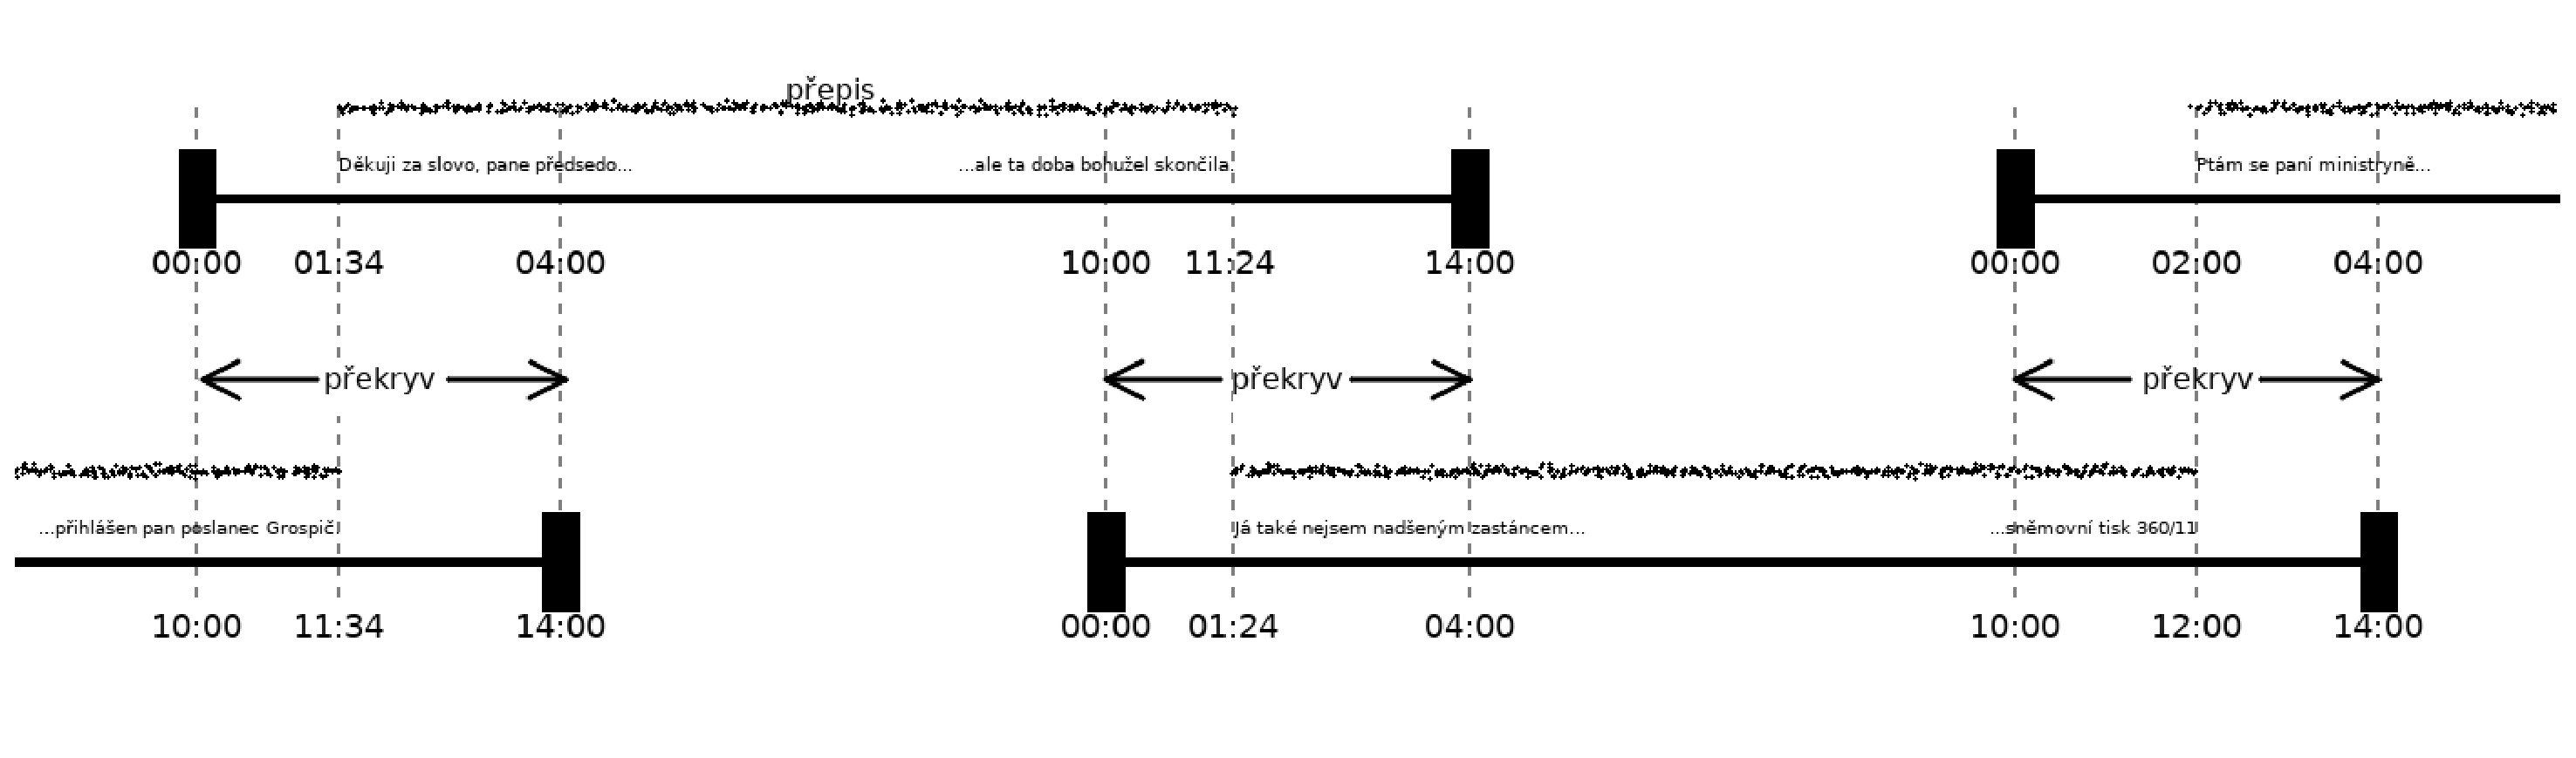
\includegraphics[scale=0.25]{rc/svolocz-overlap.eps}
\caption{Apriorní zarovnání a překryv zvukových záznamů k~přepisům. Vyobrazen je
záznam z 12. února 2020 kolem 10. hodiny. Přepis záznamu vlevo nahoře pokrývá
pozice od 01:34 do 11:24. Vpravo dole pak od 01:24 do 12:00.}
\label{fig:svolocz:overlap}
\end{figure}

Systémů pro zarovnávání dlouhých zvukových záznamů existuje několik, publikovali
je např. Moreno et al. (1998)\cite{moreno1998recursive} nebo
Hazen (2006)\cite{hazen2006automatic}. Oba jsou založeny na využití předem získaného a
zarovnaného automatického přepisu. Taktéž tento přístup využívám, ale
zjednodušený a přizpůsobený úloze.

Za použití výše zmíněného datasetu\cite{pspdata} jsem natrénoval markovovský
akustický model obdobný tomu, jenž je popsán v~kapitole~\ref{kap:asr}. Jazykový
model jsem natrénoval ze stažených stenografických přepisů. Těch je podstatně
víc než nahrávek, protože z~mně neznámého důvodu je valná část odkazů na zvukové
záznamy nefunkčních, končíc chybovým kódem 404 nebo v~menším počtu případů 403.

Pro celý korpus jsem pomocí programu julius vygeneroval automatický přepis se
zarovnáním. Automaticky vygenerovaný zarovnaný přepis každého záznamu jsem pak
porovnal s~odovídajícím manuálním přepisem pomocí Levenshteinovy metody počítání
editačních operací nad písmeny. Zjistil jsem samotné editační operace pro přechod
z~automatického přepisu k~manuálnímu a pro každé slovo v~automatickém přepisu
spočetl, kolik úprav naň připadá. Na základě toho definuji pro každé automaticky
vygenerované slovo spolehlivost párování se slovem manuálně zapsaným jako
\begin{equation}1 - \frac{e(w)}{l(w)}\end{equation}
kde $e(w)$ je počet editačních operací nad slovem $w$ a $l(w)$ je délka slova
$w$ v~písmenech.

Obrázek~\ref{fig:svolocz:align} zachycuje proces zarovnání manuálních přepisů se
zvukovým záznamem.

\begin{figure}[htpb]
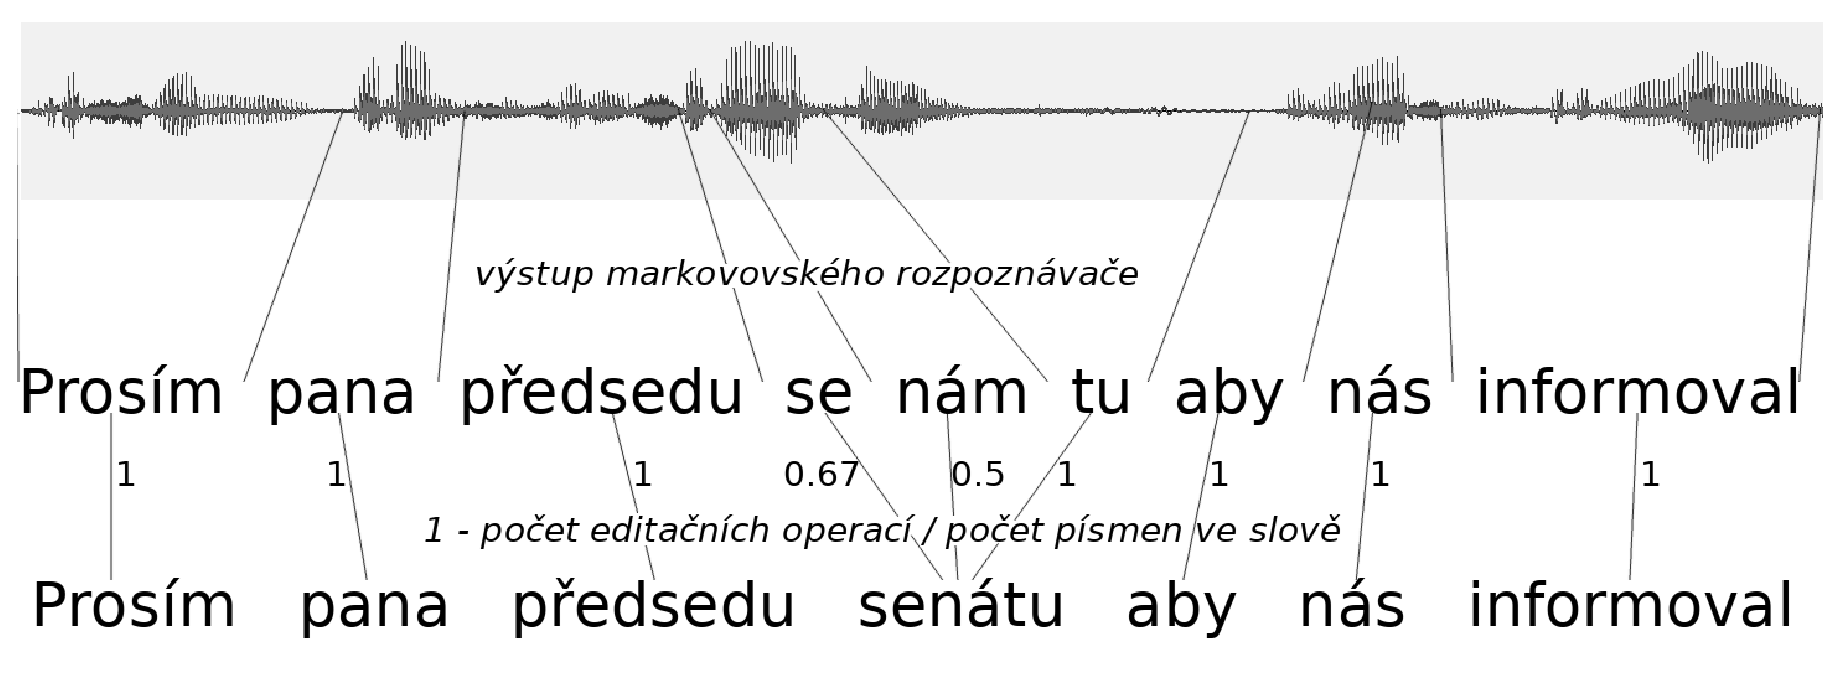
\includegraphics[scale=0.4]{rc/svolocz-align.eps}
\caption{Schéma zarovnání zvukových záznamů ke stenografickým přepisům na úrovni
slov.}
\label{fig:svolocz:align}
\end{figure}

\subsection{Tvorba potenciálních trénovacích vzorků}

Kvalita trénovacích dat pro rozpoznávání řeči závisí i na tom, jak jsou
rozdělena. Za prvé je žádoucí, aby byly trénovací vzorky podobně dlouhé
jako testovací vzorky\cite{nagorski2003search}.
V~případě automatického přepisu korpusu Karla Makoně lze
nastavit délku vstupních úseků libovolně. V~obecném případě nelze předvídat.
Za druhé je pro trénink výhodné, aby jednotlivé vzorky měly podobnou délku kvůli
efektivnímu využití operační paměti grafické procesní jednotky. Stačí jeden
dlouhý vzorek a dávka {\em (batch)} způsobí vyčerpání paměti. Naopak mnoho
kraťoučkých vzorků způsobí, že se paměť při dávce zaplní jen málo a plýtvá se
časem. Za třetí, chci-li, aby byla trénovací sada použitelná i pro ostatní,
je dobré, aby se délkou vzorků příliš neodlišovala od ostatních datových sad.

Nad to je ale důležité, aby přepis dokonale odpovídal obsahu. A protože
vyřezáváme trénovací vzorky z~delších souborů, při čemž může dojít
k~nepřesnostem, je záhodno volit místa řezu tak, aby padla pokud možno do
delších pauz v~řeči. Je to týž problém jako v~sekci~\ref{sec:segmenty}, kde je
podrobně popsán. V~tomto
případě jsem dospěl k~hranicím 12 - 30 sekund a data tak rozdělil na úseky o
délce v~tomto rozpětí.

\subsection{Výběr trénovacích vzorků}

Po rozdělení desetiminutových nahrávek na úseky vhodné délkou pro trénink je
nutné spárovat tyto úseky s~odpovídajícími úseky manuálních přepisů, a ty, které
jsou spárovány spolehlivě, zařadit do samotné trénovací množiny.
V~podsekci~\ref{subsec:svolocz:zarovnavani} jsem popsal, že máme párování
jednotlivých slov v~automatickém a manuálním přepisu s~určitou mírou
spolehlivosti a že automatický přepis je spárován se zvukovým záznamem. Zbývá
tedy vybrat úseky, které můžeme považovat za spolehlivě přepsané, a zbytek
vyřadit.

Nahrávky se překrývají tak, že z~každého čtrnáctiminutového souboru je jen deset
minut pokryto odpovídajícím přepisem, takže vyřadit musíme minimálně 29\% úseků.
Dospěl jsem k~následujícím kritériím:

\begin{enumerate}
\item{Spolehlivost prvního a posledního slova v~úseku alespoň 70\%.}
\item{Průměrná spolehlivost všech slov v~úseku alespoň 70\%.}
\item{Alespoň 5 slov v~úseku.}
\end{enumerate}

Důvodem k~zahrnutí kritéria minimální spolehlivosti krajních slov je záměr
zajistit správné hranice úseku. Druhé kritérium počítá s~průměrnou spolehlivostí
a ne třeba s~minimem, protože je přípustné, aby některá slova měla i nulovou
spolehlivost, tedy aby v~nich všechna písmena byla špatně. Iniciální přepis
obsahuje mnoho chyb, to je také důvod, proč se trénuje s~manuálním přepisem a ne
s~automatickým. Je-li ale příliš mnoho slov spárováno nespolehlivě, roste šance,
že spárování je skutečně liché. Počet slov v~úseku je mezi kritérii proto, že
u~malého počtu slov je vysoká šance náhody, při které je chybně určeno vysoké
skóre spolehlivosti nesprávně spárovaným slovům.

Pro potvrzení tvrzení, že slova s~nulovou spolehlivostí jsou přípustná, uvedu
příklad: slova \textit{,,finanční úřady dotace``} se v~jednom případě přepsala jako
\textit{,,finanční u jít dotace``}. Slova \textit{,,u``} a \textit{,,jít``} mají
obě se slovem \textit{,,úřady``} prázdnou množinu společných písmen, a tedy
nulovou spolehlivost. Přesto je obklopující fráze jako celek zarovnána správně.

Ještě vyvstává otázka, proč použít průměr a ne medián spolehlivosti v~druhém
kritériu. Je to z~toho důvodu, že liší-li se výrazně počet slov v~manuálním a
automatickém přepisu, projeví se to jako mnoho operací přidání či smazání
písmene na jednom slovu v~automatickém přepisu. V~takovém případě
mohou všechna slova mít stoprocentní spolehlivost, jen jedno hluboce pod nulou.
Takový úsek by pak byl při použití mediánu přijat, zatímco průměr výrazně negativní
hodnotu započte a úsek správně odmítne.

% TODO příklad odmítnutí pomocí průměru

\subsection{Shrnutí extrakce trénovacích dat}

Konstanty a algoritmy použité při extrakci trénovacích dat ze záznamů jednání
Parlamentu České republiky jsou jen hrubě zvoleny a je velký prostor pro jejich
odladění. Vedou ale už teď k~velmi kvalitní datové sadě o velikosti 1058 hodin.
Z~celkového počtu 539~057 úseků jich bylo 142~530 (26\%) zahrnuto do trénovací
sady. Z~celkového počtu 396~527 zavržených úseků jich 350~258 (88\%) bylo
zavrženo kvůli nespolehlivým hraničním slovům. Toto kritérium je však aplikováno
jako první, takže je v~tomto čísle zahrnuto i mnoho úseků, které by jinak byly
odmítnuty některým dalším kritériem.

Sníží-li se potřebná spolehlivost ze 70\% na 50\%, zvýší se počet přijatých úseků
o 17\%. Přidá se tak 5\% úseků z~celkového počtu. Pokud však započteme fakt, že
29\% úseků je nutně odstraněno kvůli překryvům, je celkový přírůstek ve
skutečnosti 9\% celkového počtu. Je to možnost, jak zvýšit objem trénovacích dat
za cenu zvýšení počtu úseků se špatně určenými hranicemi.

\section{Číslovky a zkratky}
\label{sec:svolocz:cislovky}

Číselných výrazů je v~parlamentních přepisech mnoho. Představují 489~880
ze~25~010~269 tokenů v~kompletním stenografickém přepisu, to jsou téměř dvě
procenta. Ve výše popsaných trénovacích datech je aspoň jedno číslo ve 24\%
vzorků.

Původní moje řešení spočívalo v~zahrnutí číslic do abecedy a tedy
v~pokusu o přepis číselných výrazů přímo na číslice. V~systému rozpoznávání řeči
natrénovaném na těchto datech, popsaném v~následující sekci, bohužel výsledkem bylo, že
číselné výrazy se vždy přepsaly na prázdný řetězec.

K~problému se lze postavit čtyřmi způsoby:
\begin{enumerate}
\item{ignorovat ho,}
\item{vyřadit číslice z~trénovacích dat,}
\item{manuálně číslice rozepsat do slov,}
\item{číslice rozepsat automaticky.}
\end{enumerate}

První možnost ignorování problému asi netřeba rozebírat.
Vyřazení vět s~číslicemi je snadný a použitelný přístup, ale byla by škoda
přijít o čtvrtinu trénovacích dat a o drtivou většinu příkladů číslovek.
Manuální přepis by byl jistě ideální, ale vzhledem k~objemu dat pro mne
nerealizovatelný. Zbývá se tedy pokusit o čtvrtou možnost.

Pro automatický rozpis číslic do slov lze využít hotového aparátu: iniciálního
přepisu a algoritmu pro zarovnávání se stenografickým přepisem.

Rozpis provádím ve dvou krocích:
\begin{enumerate}
\item{vygenerování možných čtení číslicového výrazu,}
\item{výběr nejpravděpodobnější varianty.}
\end{enumerate}

Pro generování možných čtení čísel jsem vyšel z~algoritmu použitého v~modulu pro
Perl \texttt{Lingua::CS::Num2Word}, který jsem doplnil o řád miliard pro
kardinální číslovky, rozšířil tak, aby se místo jedné varianty generovaly
pokud možno všechny gramaticky přípustné, a zahrnul podporu genitivu a
akuzativu, decimálních a ordinálních číslovek, dat a hodin.

Ve stenografických přepisech před dalším zpracováním rozvedu všechny tokeny
obsahující číslice do variant rozpisu a při zarovnávání s~iniciálním
automatickým přepisem vyberu tu variantu, která má nejmenší editační vzdálenost.

Spolu s~číslicemi expanduji také zkratky a symboly. Např. velmi častý symbol
paragraf (§) rozepisuji do variant {\em paragraf, paragrafu, paragrafů,
paragrafem, paragrafech}, které se podle iniciálního přepisu vyskytují jako
jediné časté. Dalšími častými zkratkami s~různými variantami rozpisu jsou {\em
čl. -- článek / článku / ..., odst. -- odstavec / odstavce / ..., tzv. --
takzvaný / takzvaného / ...}.

Po provedení expanze se podobnost stenografického a iniciálního automatického
přepisu zvýšila, což se odrazilo i na zvýšení počtu přijatých úseků z~26\% na
35\%. Množství trénovacích dat v~hodinách vzrostlo o 86, tedy na 1144.

O využití datové sady pro rozpoznávání řeči pojednává sekce~\ref{sec:csasr:results}.


\chapter{Automatický přepis}
\label{kap:asr}

% - množina fonémů
% - vektorový formát
% - HMM X CNN
% - HTK X Kaldi X sphinx X Bourlard X TensorFlow
% - Monofonémy X trifonémy
% - mixtury
%   - individuální
%   - globální
%   - na monofonémech vs. trifonémech

Koncept celého projektu se zakládá na~přítomnosti automatického přepisu a jeho
následném zdokonalování. Jelikož nebyl k~dispozici uspokojivý hotový nástroj pro
získání automatického přepisu, nezbylo než jej vytvořit.

Zjednodušený řetězec vedoucí od~zvukových dat k~jejich přepisu v~našem případě
vypadá takto:\begin{enumerate}
\item{sběr trénovacích dat,}
\item{stavba akustického modelu,}
\item{stavba jazykového modelu,}
\item{automatické rozpoznávání.}
\end{enumerate}

V tomto řetězci je stavba akustického modelu patrně nevyznamnějším článkem a
sama tvoří řetěz o~mnoha článcích. V~této kapitole pojednáme o~krocích
podniknutých k~jeho sestavení, experimentech a různých volbách.

Do~užšího výběru potenciálních platforem tvorby akustického modelu jsem zařadil
starší systém \textit{HTK}\footnote{hmm toolkit; Hidden Markov Model Toolkit} a
modernější \textit{Kaldi}. HTK pomyslný konkurz nakonec vyhrál díky zkušenostem
mého konzultanta Mgr. Nina Peterka, Ph.D. s~tímto systémem, z~nichž jsem mohl
čerpat.

Akustický model jsem trénoval výhradně z~vlastníh dat.
% Obětoval jsem tedy
% potenciální přínos většího množství trénovacích dat a upřednostnil trénování
% přímo na~konkrétního mluvčího.
%TODO: od kdy se vyplatí dělat model na konkrétního mluvčího?

Tvorba akustického modelu probíhala podle návodu v~manuálu k~HTK, \textit{HTK
Book}. V~hrubých rysech probíhá takto:

\begin{enumerate}

\item{Vytvoření počátečních modelů}

Modeluje se skrytými markovovskými řetězci. Všechny fonémy se inicializují jako
shodné. Každý foném je reprezentován pěti stavy (vstupním, výstupním a třemi
vnitřními). Přechodové pravděpodobnosti se nastaví tak, aby byly možné jen
kýžené přechody, to jest ze~vstupního do~druhého a z~každéhu z~vnitřních stavů
do~sebe samého nebo do~následujícího. Konkrétní pravděpodobnosti nejsou
podstatné, ale použil jsem 60\% pro setrvání a 40\% pro postup ve~druhém a
třetím stavu a 70\% pro setrvání a 30\% pro postup ze~čtvrtého do~výstupního.
Střed a variance jsou určeny identicky podle globálních hodnot.

Kromě vlastních fonémů (viz níže oddíl~\ref{sec:ac:fonetika}) přidám ještě foném
pro~ticho (\textit{sil}).

Pro kódování používám formát MFCC s~první a druhou derivací, nultým koeficientem
a kepstrální normalizací (\texttt{MFCC\_0\_D\_A\_Z} v~notaci HTK).

Následují dvě iterace tréninku Baum-Welchovým algoritmem\cite{welch2003hidden}.

\item{Přidání modelu pro krátkou pauzu}

Z~modelu pro ticho se odvodí model pro krátkou pauzu tak, že se povolí přechod
rovnou z~druhého do~čtvrtého stavu a zpět, aby byl model robustnější a mohl
modelovat pauzu mezi slovy, která je nezřídka nulová.

Trénuje se opět dvěma iteracemi BW-algoritmu.

\item{Nucené zarovnání a odvržení zmetkových vzorků}

Pomocí Viterbiho algoritmu~\cite{forney1973viterbi} se provede tzv.
\textit{forced alignment}, tzn. nucené zarovnání na~úrovni fonémů. Jinými slovy
určí se přesný čas, kde začíná a končí který foném. Při tom se určí hranice, pod
kterou když klesne \textit{likelihood} daného přepisu na~základě odpovídající
nahrávky, tato se z~trénovacích dat odstraní jako pravěpodobně vadná. Následují
další dvě iterace BW-algoritmu.

\item{Přepočítání variance}

Variance modelů byla určena podle původní trénovací sady. Nyní jsme z~ní
vyřadili některé vzorky, proto proběhne její přepočtení, opět následované dvěma
trénovacími iteracemi.

\item{Přechod k~trifonémům}
\label{item:htktrain:triphones}

Z~nuceného zarovnání máme přepis obohacený o~konkrétní fonetické realizace. Z~té
se nyní snadno vytvoří transkripce trifonémová tak, že ke každému fonému přidáme
jeho levý a pravý kontext, pokud nejsou na~začátku nebo na~konci věty.

Je-li fonémů 45, pak trifonémů je až $45^3 = 91125$. Ne všechny se v~trénovacích
datech objeví. V~praxi jich mám kolem 14 tisíc. Pokud by každý trifoném měl
vlastní separátní model, došlo by k~opačnému problému než v~případě monofonémů,
totiž že by celkový model měl příliš mnoho parametrů. Přechodové matice mohou
všechny trifonémy odvozené od jednoho monofonému sdílet. Avšak které trifonémy
mají sdílet varianci a které mají mít vlastní, je třeba rozhodnout opatrněji.

Pro určení, které modely je vhodné sloučit, používám rozhodovací stromy.
Na~základě předem definovaných kritérií se u~každého emitujícího stavu každé
skupiny trifonémů provede rozdělení na~dva shluky, což umožní zvýšení
\textit{log likelihood} dat. Vybere se kritérium, které ji zvýší nejvíce a
postup se opakuje, dokud zvýšení neklesne pod~danou hranici. Takto získané
shluky se pak sloučí do jednoho logického trifonému.

\item{Štěpení mixtur}

Posledním krokem ve~zvětšování komplexity modelu je štěpení tzv.~\textit{mixtur}
(z~angl. \textit{mixtures}). Spočívá v~tom, že se přesněji modelují variantní
realizace jednotlivých fonémů. Daný foném v~jednom stavu HMM pak není modelován jednou gaußovskou
distribucí, nýbrž složením několika. Každá má svůj střed, svoji varianci a svoji
váhu, jejichž celkový součet musí být roven jedné.

Štěpí se vnitřní stavové modely jednotlivých fonémů. Optimální počet
mixtur je tedy potřeba zjistit pro trojnásobek počtu použitých trifonémů. To
jsou řádově tisíce až desítky tisíc. V~okamžiku psaní tohoto textu používám 8444
reálných trifonémů, 13746, počítám-li i ty virtuální. To znamená přes dvacet pět
tisíc distribucí, u~nichž je potřeba určit optimální počet mixtur.

Aby byl úkol aspoň aproximací dosažitelný, je třeba hledat efektivněji než
prohledáváním celého prostoru hrubou silou. První pomocí zde je, že modely jsou
na sobě více méné nezávislé: Nalezneme-li optimální počet mixtur pro jeden
z~nich, nemělo by to ovlivnit optimální počet mixtur u~jiného.

Rozštěpení u~jednoho modelu proběhne tak, že se mixtura s~největší vahou
rozštěpí na dvě totožné, jen jedna dostane malinko větší váhu než druhá, aby se
při trénování mohly rozejít. To se provede u~všech vnitřích stavů všech
logických fonémů, t.j. u~všech markovovských modelů. Provedou se čtyři trénovací
iterace a úspěšnost se vyhodnotí na~sadě heldout.

Pokud u~některé mixtury klesne její váha pod~daný práh, vymaže se, čímž se
zamezí zbytečnému nárůstu parametrů a není proto potřeba zkoušet štěpit
jednotlivé modely samostatně. Arci, takovým způsobem jsem nikdy nedosáhl lepšího
výsledku, než štěpením všech modelů najednou.

Závislost úspěšnosti na~počtu mixtur není monotónní, proto ve~štěpení pokračuji,
i když někdy úspěšnost klesne. Konkrétně zastavím štěpení, pokud úspěšnost
klesne o~více než 30\% oproti nejvyšší dosažené nebo pokud klesne více než
třikrát za~sebou, ale nikdy když je mixtur méně než 16.

Pokud je foném gaußiánem modelován dobře, rozdělení na dvě mixtury
nijak nepomůže. Navíc pokud rozdělíme dostribuci příliš, dojde snadno
k~přetrénování. Je proto potřeba nalézt optimální počet mixtur pro každý
jednotlivý trifoném.

\end{enumerate}

\section{Segmentace}

Zpravidla jeden zvukový soubor odpovídá jednomu přetočení magnetofonové pásky,
obvyklá délka je tedy 45 až 120 minut. Takto dlouhé úseky nelze použít ani jako
trénovací příklady ani jako cíl automatického rozpoznávání.

Celá aplikace je pojata jako nástroj pro~zdokonalování automatického přepisu,
takže vychází z~předpokladu, že nějaký přepis již existuje. Vycházeje z~téhož
předpokladu při~segmentaci, realizoval jsem ji tak, že zvukový soubor se rozdělí
na~úseky odpovídající jednotlivým větám v~přepisu, ne však delší než patnáct
sekund. Pokud by věta byla delší, rozdělí se u nejbližšího slova
před~patnáctisekundovou hranicí.

V~případě, že pro daný záznam zatím žádný přepis neexistuje, rozdělí se naivně
na~patnáctisekundové úseky.

Nutno dodat, že rozdělování podle automaticky rozpoznaných hranic vět by šlo
snadno vylepšit. Jde-li o~ručně přepsaná data, jsou hranice vět dobrým vodítkem,
ale u~automaticky přepsaných by bylo lépe rozdělovat podle ticha mezi slovy.

\section{Fonetika}
\label{sec:ac:fonetika}

\subsection{Fonetický přepis}

Trénovací data pro akustické modelování pomocí HTK mají formu párů
parametrizovaných zvukových souborů (v~mém případě MFCC) a textových souborů,
obsahujících fonetický přepis. Ten se může získat různými způsoby. Lze ručně
anotovat data do~fonetického i běžného přepisu, což se ale běžně nedělá. Běžně
se trénovací přepisy do fonetických převádějí automaticky. U jazyků
s~nepravidelnou výslovností, jako je angličtina, je často nejlepší použít
robustní výslovnostní slovník a v~případě jeho nedostatečnosti se uchýlit
k~pravidlové výslovnosti, popř. anotovat mimoslovníková slova ručně.

Čeština skýtá se svojí téměř deterministickou a navíc relativně jednoduchou
fonetikou možnost používat primárně pravidlový přepis. Výjimky pak lze ošetřit
slovníkem. Vzhledem k~tomu, že slovní zásoba Karla Makoně je svérázná a
netypická, vydal jsem se právě touto cestou, neboť i kvalitní robustní slovník
by zde byl nedostatečný a svou obsáhlostí zbytečný.

Pro zachycení výjimek z~výslovnostních pravidel mám vlastní řešení. Uživatelé
přepisovací aplikace jsou instruováni slova s~nepravidelnou výslovností označit,
viz kapitolu \ref{kap:webove-rozhrani}. Když se toto stane, výslovnost spárovaná
se~zápisem se přidá do~výslovnostního slovníku jako výslovnostní varianta.
Výslovnostní slovník je implementován jako tabulka v~relační databázi. Tím, že
se přidá výslovnostní varianta, se ošetří případ, že by mluvčí vyslovil slovo
foneticky. Pokryjí se tím nejen cizí slova, jako \textit{Marie Markéta Alacoque}
[\fontspec{DoulosSIL}alakok\normalfont], nýbrž také ledabyle vyslovená slova,
jako \textit{protože} [\fontspec{DoulosSIL}brʒɛ\normalfont].

\subsection{Fonémy}

% TODO cite

Používám základní fonémy českého jazyka~\cite{palkova1992fonetika}
reprezentované pomocí PACal~\cite{nouza1997phonetic}. Kromě základních fonémů
používám dvojhlásky, ticho a krátkou pauzu. Ráz (glotální plozivu) nevyznačuji,
jakož ani neřečové události.
V~tabulce~\ref{tab:phones} jsou fonémy uvedeny.

\begin{table}[htpb]
\fontspec{DoulosSIL}
\begin{center}
\begin{tabular}{|l|l|l|l||l|l|l|l|}
\hline
IPA & PACal & grafém & IPA & PACal & grafém \\
\hline
a  & a   & a      &     ɱ  & mg  & tra\underline{m}vaj \\
aː & aa  & á      &     n  & n   & \underline{n}e \\
aʊ̯ & aw  & au     &     ŋ  & ng  & ta\underline{n}k \\
b  & b   & b      &     ɲ  & nj  & \v{n} \\
t͡s & c   & c      &     o  & o   & o \\
t͡ʃ & ch  & č      &     oː & oo  & ó \\
d  & d   & d      &     oʊ̯ & ow  & ou \\
ɟ  & dj  & \v{d}  &     p  & p   & p \\
d͡z & dz  & dz     &     r  & r   & r \\
d͡ʒ & dzh & dž     &     r̝̊  & rsh & t\underline{\v{r}}i \\
ɛ  & e   & e      &     r̝  & rzh & \underline{\v{r}}íz \\
ɛː & ee  & é      &     s  & s   & s \\
eʊ̯ & ew  & eu     &     ʃ  & sh  & š \\
f  & f   & f      &     t  & t   & t \\
g  & g   & g      &     c  & tj  & \v{t} \\
ɦ  & h   & h      &     ʊ  & u   & u \\
i  & i   & i      &     uː & uu  & ú, \r{u} \\
iː & ii  & í      &     v  & v   & v \\
j  & j   & j      &     x  & x   & ch \\
k  & k   & k      &     z  & z   & z \\
l  & l   & l      &     ʒ  & zh  & ž \\
m  & m   & \underline{m}ák
                  &        & sil & \\
   &     &        &        & sp  & \\
\hline
\end{tabular}
\caption{použité fonémy: IPA, PACal a nejčastější odpovídající
grafém}\label{tab:phones}
\end{center}
\end{table}
\normalfont

V~závislosti na~množství trénovacích dat bylo vhodné nahradit některé fonémy
častějšími podobnými. V~tabulce~\ref{tab:phonesed} jsou záměny vyčísleny.
\begin{table}[htpb]
\fontspec{DoulosSIL}
\begin{center}
\begin{tabular}{|r|l|l||l|l|}
\hline
&
\multicolumn{2}{|c||}{před záměnou} &
\multicolumn{2}{|c|}{po záměně} \\
\hline
& IPA & plz. & IPA & plz. \\
\hline
    & ɱ  & mg & m & m \\
    & aʊ̯ & aw & a ʊ & a u \\
    & oː & oo & o & o \\
\** & d͡z & dz & t͡s & c \\
    & d͡ʒ & dzh & t͡ʃ & ch \\
\** & eʊ̯ & ew & ɛ ʊ & e u \\
\hline
\end{tabular}
\caption{použité záměny fonémů; hvězdičkou jsou vyznačeny záměny použité ještě
v~době psaní textu}\label{tab:phonesed}
\end{center}
\end{table}
\normalfont

\section{Rozdělení dat}

Pro natrénování modelu strojovým učením je potřeba trénovacích dat a pro
vyhodnocení jeho úspěšnosti dat testovacích, která ve~fázi trénování nesmí být
algoritmem spatřena. Při trénování samotném se pak mnohdy používá vyhrazených,
tzv.~\textit{heldout} dat pro průběžné měření úspěšnosti. V~případě trénování
akustického modelu s~použitím HTK je tomu nejinak. Heldout data jsou používána
pro zjištění optimálního počtu mixtur modelů jednotlivých fonémů, a testovací
pro závěrečné vyhodnocení.

Anotovaná data mi přibývala velice pozvolna a začínal jsem s~několika minutami,
ovšem přírůstky byly časté. Nemohl jsem si tedy dovolit udělat od~začátku pevnou
testovací sadu, kterou bych používal po~celou dobu provádění experimentů. Místo
toho jsem s~každou novou dávkou anotovaných dat celou sadu rozdělil podle vět
v~poměru 18:1:1 do trénovací, heldout a testovací sady. Tak jsem měl neustále
vyvážený poměr jednotlivých datových sad. Zřejmou velkou nevýhodou bylo, že
nešlo spolehlivě porovnávat výsledky jednotlivých experimentů vzhledem
k~variabilní testovací sadě.

Až když jsem měl několik desítek hodin anotovaných dat, vyhradil jsem si fixní
testovací sadu. Běžně se testovací sada vybere jako náhodná podmnožina vzorků
z~trénovací sady tak, aby měla kýženou velikost. V~mém případě vzorků zvíci
hodinových nahrávek jsem sadu určil manuálně jako úsek druhé až jedenácté minuty
(tedy deset minut minutu po~začátku) v~pěti nahrávkách,
\begin{enumerate}
\item{jedné kazety z~roku 1976,}
\item{jedné z~roku 1982,}
\item{jedné z~roku 1986,}
\item{jedné z~roku 1990 a}
\item{jednoho nedatovaného kotouče.}
\end{enumerate}

Sadu heldout nyní vybírám jako každou čtyřicátou větu. Z~každé dvacáté jsem
snížil na~polovic nejen abych neplýtval trénovacími daty, nýbrž také protože
vyhodnocování mixtur zabírá při trénování zdaleka nejvíce času, a ten je přímo
úměrný velikosti sady heldout.

\section{Spojování trifonémů}

Pro slučování modelů jednotlivých trifonémů, jak zmiňuje
bod~\ref{item:htktrain:triphones} seznamu kroků trénování pomocí~HTK, je
zapotřebí rozhodovacích stromů. Pro jejich tvorbu je potřeba ručně vytvořit
otázky, na základě nichž, bude algoritmus dělit fonémy do shluků. K~tvorbě
otázek můžeme použít lingvisticky motivovanou kategorizaci v~naději, že aspoň
některé lingvistikou definované kategorie budou tvořit konzistentní shluky
z~pohledu trénovacích dat. Pro tvorbu otázek jsem vycházel z~předlohy pro
angličtinu, jak je v HTK Book a z~kategorizace českých hlásek na Wikipedii ({\em
https://cs.wikipedia.org/wiki/Fonologie~češtiny}).

\section{Experiment s kepstrální normalizací}

Kepstrální normalizace je standardní technikou pro kompenzaci různorodých
akustických podmínek v~rámci trénovacích a testovacích dat, viz Viikki a Laurila
1998\cite{viikki1999cepstral}. Princip této techniky spočívá v~tom, že se ode
všech melfrekvenčních kepstrálních koeficientů odečte jejich průměr z~akusticky
konzistentního úseku. Já toto poněkud hrubiánsky činím na celých nahrávkách,
které nejsou vždy akusticky konzistentní, ale často ano a nalezení akusticky
podobných množin je jedním z~mých plánů pro budoucí práci.

Nabízí se však otázka, zda má smysl odečítat průměr z~celé nahrávky, nebo by to
mělo být jen z~řečových událostí, tedy s~vynechaným tichem (šumem, hluky atd.)
Tato idea, přišedší ke mně od Davida Klusáčka, mne zaujala natolik, že jsem se
ji pokusil ověřit. Vytvořil jsem proto jednak metadata s~časovými pozicemi všech
izolovaných řečových událostí na základě zarovnaného automatického přepisu, kde
jsem vynechal všechny fonémy \texttt{sil} a \texttt{sp}, a jednak sadu skriptů
pro manipulaci se soubory MFCC.

Celkový přínos pro úspěšnost rozpoznávání byl nulový, ale aparát pro dekódování
a manipulaci souborů MFCC považuji za vítaný vedlejší produkt.

\section{Aktivní učení}

Aktivní učení spočívá ve vhodném výběru trénovacích dat, viz např. Cohn
1996\cite{cohn1996active}. V~mém případě trénovací sada postupně roste a je tedy
nabíledni techniky aktivního učení využít tak, aby se získávala co nejvhodnější
trénovací data.

Podnikl jsem experiment, ve kterém jsem 2\% slova s~nízkou {\em confidence
measure (c.m.)} červeně podtrhl přerušovanou čarou, jejíž sytost spojitě rostla
s~klesající c.m. Instruoval jsem pak uživatele aplikace, aby přednostně
přepisovali věty, které jsou opticky co nejčervenější. Bohužel přirozené puzení
uživatelů přepisovat nahrávku kompletně a lineárně od začátku způsobilo, že
přepisů, kde se tato instrukce dodržuje, je zcela mizivé množství.

Druhý experiment spočíval v~tom, že webová aplikace sama vybírala věty pro
přepis na základě toho, kolik obsahovala slov s~nízkou c.m. Uživatelé pak byli
instruováni, aby nahrávku jen poslouchali, a opravu vložili, až když se
přehrávání samo přeruší. Tento pokus skončil ještě palčivějším neúspěchem, neboť
změna v~chování aplikace byla pro uživatele natolik nepříjemná, že jsem je
raději navrátil do původního.

\chapter{Webové rozhraní}
\label{kap:webove-rozhrani}

\section{Porovnání s~jinými scénáři}

Mým dílčím cílem je co nejlepší ortografický\footnote{Na pravopis jako takový se důraz
neklade. Ortografickým přepisem myslím standardní zápis.} a fonetický přepis
tisícihodinového korpusu jednoho mluvčího rozděleného do přibližně hodinových
celků. Existuje skupina lidí, které nahrávky zajímají. Tito lidé představují na
jednu stranu potenciál, který mohu využít pro svůj účel, a na druhou stranu
moji, abych tak řekl, cílovou skupinu, tedy ty, jimž bude produkt sloužit.

Webová aplikace by tedy měla skloubit tyto dva účely:
\begin{enumerate}
\item{sloužit uživatelům, aby mohli  materiál co nejlépe konzumovat,}
\item{ponouknat uživatele, aby dali co nejkvalitnější přispěvek.}
\end{enumerate}

Pokud je mi známo, není žádného projektu se srovnatelným východiskem. Můžeme
však porovnávat jednotlivé aspekty, vyskytující se v~jiných aplikacích.

\subsection{Programy pro přepis}
\label{ssec:diff:trans}

Nejpodobnější a přitom rozšířený typ aplikace je pro přepis mluveného slova
člověkem. Porovnejme tyto dva úkoly a zpytujme hlavní rozdíly. K~porovnání
vezměme
\begin{enumerate}
\item{
    Transcriber\footnote{trans.sourceforge.net}, klasický svobodný program
    napsaný v~TCL,
}
\item{
    oTranscribe\footnote{otranscribe.com}, svobodný moderní webový přepisovací
    nástroj a
}
\item{
    Transcribe\footnote{transcribe.wreally.com}, komerční webový přepisovací
    nástroj.
}
\end{enumerate}

Každé číslo v~seznamu níže označují program, pro který platí ten který výrok. Ku
příkladu z~nich jen Transcriber umožňuje anotaci mluvčích, proto u druhé položky
stojí pouze číslo (1).



\noindent
\begin{tabularx}{\textwidth}{
    @{\hspace{1.5em}}% Space for left bullet
    >{{\hsize=0.9\hsize}\leavevmode\llap{\textbullet~}\raggedright}% Left bullet + formatting of column
    X% Left column specification
    @{\hspace{0.2em}}
    >{\hsize=0.2\hsize}
    X
    @{\quad\hspace{1.5em}}% Space between columns + right bullet space
    >{\leavevmode\llap{\textbullet~}\raggedright\arraybackslash}% Right bullet + formatting of column
    X% Right column specification
    @{}% No column space on right
  }
  \em{přepisovací programy}: & & \em{moje aplikace}: \\
  jsou optimalizované pro pořízení přepisu od nuly; &
    (1,2,3) &
      vždy vychází z~existence předchozího přepisu; \\

  umožňují anotaci mluvčích; &
    (1) &
      předpokládá, že všechna slova pocházejí od jednoho mluvčího; \\

  nepotřebují kontrolu kvality: uživatel může přepisovat dle libosti a konečným
  měřítkem je jeho vlastní spokojenost; &
    (1,2,3) &
      vyžaduje přesnost přepisu neboť tento je použit pro trénování
      statistických modelů; \\

  zarovnávají na úrovni frází, pokud vůbec; &
    (1)\footnote{
        Transcriber explicitně zarovnává text s mluveným slovem, oproti zbylým
        dvěma, které toliko umožňují přidání časových značek do přepisu.
    } &
      zarovnává na úrovni slov, interně na úrovni fonémů; \\

  točí se kolem uživatele: každý může přepisovat jakákoliv data si zvolí; &
    (1,2,3) &
      točí se kolem dat: sbírka nahrávek je středobodem aplikace a přepisovat
      lze pouze ji; \\

  předpokládá, že přepisovat je uživatelův záměr; &
    (1,2,3) &
      předpokládá, že uživatel chce poslouchat, popř. vyhledávat nebo číst
      s~poslechem, a k~přepisu ho nutno přimět; \\

  nesdílejí data mezi uživateli; &
    (1,2)\footnote{Transcribe podporuje kolaborativní přepis} &
      musí počítat s~kolizemi. \\
\end{tabularx}

\vspace{5mm}

Navzdory těmto odlišnostem se v~přepisovacím softwaru skrývá mnoho poučného.
Snadnost provádění běžných úkonů, jako pozastavení a obnovení přehrávání či
posun jsou pro uživatelský prožitek (UX) stěžejní a tím i pro množství a kvalitu
příspěvků. I způsob synchronního zobrazení textu se zvukem má velký dopad a
v~potenciálních přístupech je značná svoboda pro variaci.

\subsection{Wiki}

Tam, kde se moje aplikace odchyluje od přepisovacích programů, tam do značné
míry připomíná wiki: komunitní platformu, která slouží uživatelům včetně
přispěvatelů, ale kde kvalita příspěvků je podstatná, zatímco samotná
spokojenost přispěvovatelova nemá takovou důležitost.

Jeden podstatný rozdíl oproti wiki je, že wiki je kreativní, kdežto náš úkol je
mechanický. Uživatel má pramálo prostoru pro vlastní invenci: poskytnutí jiného
než doslovného přepisu se vnímá jako chyba.

Populární wiki mají dobrá opatření pro konflikty v~editacích, což je oblast, kde
bych se mohl nechat poučit. Zatím k~tomu ale nebyl důvod, protože pokud vždy
použiji nejnovější verzi každého segmentu, výsledek zůstane konzistentní, i když
segment od uživatele A padne do širšího přepisu od uživatele B.

V přepisu, jak se zobrazuje návštěvníkům, nově odeslaný segment přepisu vždy
přepíše stávající verzi, ale všechny příspěvky udržuji v~databázi, takže každý
lze zvrátit {\em (undo)}, také lze shlukovat příspěvky podle jejich autora atd.,
ale zatím něčeho takového nebylo zapotřebí.

\subsection{Korpusy}

Tento projekt není prvním, který zahrnuje komunitní péči o korpus. Za zmínku
stojí Manually annotated sub-corpus\cite{ide2010manually}, kde se anotace různého
druhu střádají od dobrovolníků. Dále Wikicorpus\cite{reese2010wikicorpus},
korpus článků z~Wikipedie s~určitou úrovní lingvistické anotace. Můj projekt
může s~těmito v~budoucnu dosáhnout značné podobnosti, až se hlavní bod zájmu
stočí od samotného přepisu k~anotaci.

Je zde také CzEng\cite{bojar2008czeng}, česko-anglický paralelní korpus, kde
velká část překladů pochází od dobrovolníků. Podobnost ve východisku je zde
pozoruhodná, neboť v~obou projektech se z~původního materiálu dojde k~derivátu
pomocí počítačového zpracování a chyby v~něm se pak komunitně opravují.
V~případě CzEngu jde o strojový překlad, v~mém o strojový přepis. Nicméně
specifika projektů přinášejí odlišné problémy a diktují odlišné přístupy.

Marge (2009)\cite{5494979} zkoumá použití platformy Mechanical Turk k~získání
přepisů mluveného slova. Mihalcea (2004)\cite{mihalcea2004building} prezentuje
webové rozhraní pro desambiguaci významu slov (word-sense disambiguation) a
zaměřuje se především na ošetření neshod mezi anotátory.

\section{Popis webové aplikace}

Aplikace sestává z~několika {\em pohledů\footnote{Pohled ve smyslu ,,view''
z~architekturního přístupu ,,model - view - controller''. Podobně jako autoři
frameworku Django, pojmem pohled - view míním jednu stránku definovanou cestou
v~URL i s~její funkcionalitou.}}:
\begin{enumerate}
\item{úvodní stránky se seznamem nahrávek, kde každý záznam odkazuje na detailní
pohled,}
\item{detail nahrávky, kde je možné přehrávání, zobrazuje se přepis tento se dá
editovat,}
\item{výsledky vyhledávání, kde každý záznam obsahuje úryvek odpovídající
vyhledávanému dotazu a odkazuje na příslušnou pasáž nahrávky v~detailním
pohledu,}
\item{různé statické podstránky s~obecnými informacemi, manuálem atd.}
\end{enumerate}

Úvodní stránka má
dvousloupcový formát, kde vlevo je rozbalovací seznam kategorií a vpravo
lineární seznam nahrávek. Jednotlivé kategorie jsou pak skrolovacími odkazy
do~pravého sloupce a podle stupně skrolování se příslušná kategorie sama
rozbalí (tzv. scrollspy).

Pro lepší přehlednost a v souladu s principem Separation of Concerns je seznam
nahrávek pouze na~úvodní stránce.

Podrobněji se budu zabývat pouze pohledem detailu nahrávky.
Obrázek~\ref{fig:scn1lab} ukazuje rozhraní v~průběhu přehrávání.
Obrázek~\ref{fig:scn2lab} ukazuje rozhraní při editaci segmentu.

\begin{figure}[htpb]
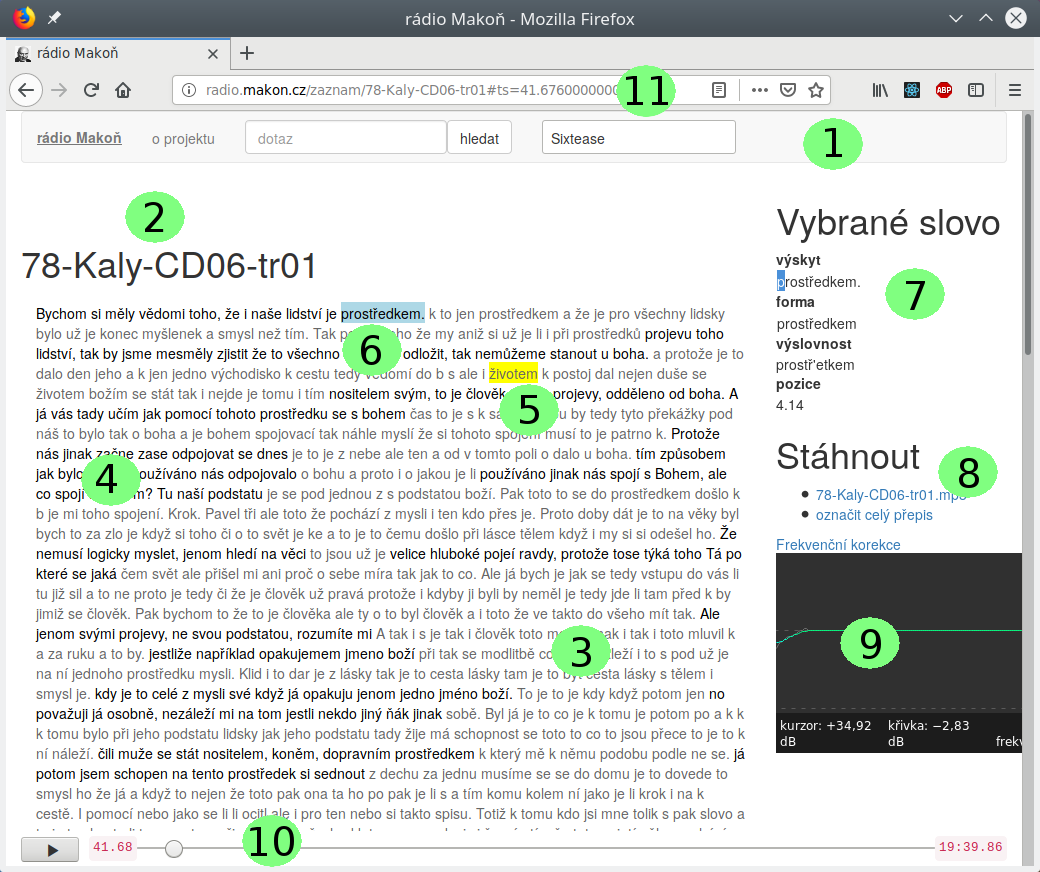
\includegraphics[scale=0.6]{rc/radio-makon-cs-1-lab.png}
\caption{webové rozhraní při přehrávání}
\label{fig:scn1lab}
\end{figure}

Vysvětliky k~obrázku~\ref{fig:scn1lab}:
\begin{enumerate}
\item{
    Záhlaví a v~něm
    \begin{itemize}
    \item{jméno aplikace odkazující na úvodní stránku,}
    \item{odkaz na informace o projektu,}
    \item{vyhledávací políčko,}
    \item{vstupní pole pro uživatelovu přezdívku;}
    \end{itemize}
}
\item{Identifkátor nahrávky;}
\item{Automaticky přepsané segmenty v~šedi;}
\item{Manuálně přepsané segmenty v~černi;}
\item{Právě přehrávané slovo zvýrazněné žlutým pozadím;}
\item{Označené slovo zvýrazněné modří st. regent na pozadí;}
\item{
    Informace o označeném slově:
    \begin{itemize}
    \item{
        výskyt: slovo s~kontextuálním velkým písmenem,
        interpunkcí, jak se nachází v~textu
        (navíc právě editované, jak prozrazuje označené iniciální písmeno),
    }
    \item{forma: normalizovaná slovní forma, jak se objevuje ve slovníku,}
    \item{
        výslovnost: český fonetický zápis použité výslovnosti (viz
        podsekci~\ref{ssec:respelling}),
    }
    \item{
        pozice: čas v~sekundách od začátku nahrávky do začátku slova;
    }
    \end{itemize}
}
\item{
    Ukládání:
    \begin{itemize}
    \item{přímý odkaz k~celé nahrávce ve formátu mp3,}
    \item{označení celého přepisu pro snadné vložení (copy-paste);}
    \end{itemize}
}
\item{Grafický ekvalizér pro kompenzaci úzkopásmového šumu;}
\item{
    Ovládací prvky přehrávání:
    \begin{itemize}
    \item{tlačítko pro pozastavení / pokračování,}
    \item{současná pozice,}
    \item{posuvník (scrollbar) přehrávání,}
    \item{celková délka nahrávky;}
    \end{itemize}
}
\item{aktuální pozice reflektovaná v~URL;}
\end{enumerate}

\begin{figure}[htpb]
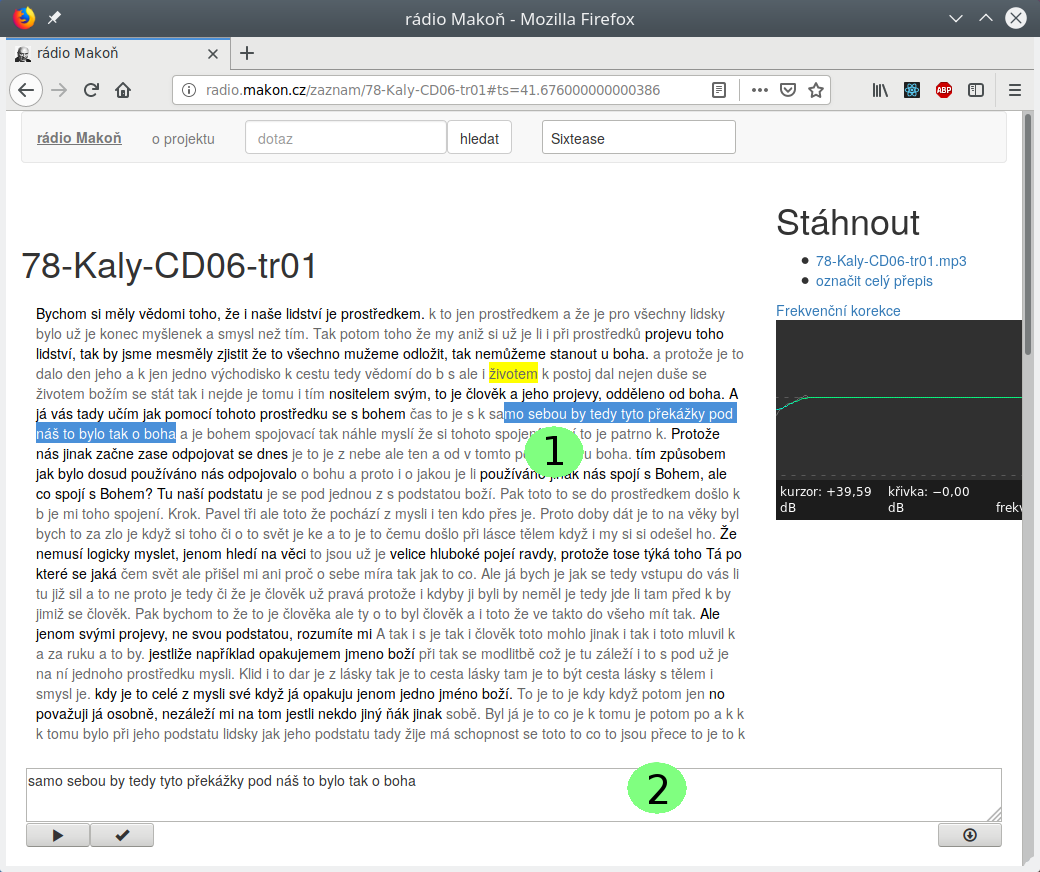
\includegraphics[scale=0.6]{rc/radio-makon-cs-2-lab.png}
\caption{rozhraní ve stavu editace segmentu}
\label{fig:scn2lab}
\end{figure}

Vysvětlivky k~obrázku~\ref{fig:scn2lab}:
\begin{enumerate}
\item{
    Označení textového úseku myší definuje segment k~editaci tak, že označené
    části slov se doplní na celá;
}
\item{
    Editační okénko a v~něm:
    \begin{itemize}
    \item{textové pole (textarea) předvyplněná stávajícím přepisem,}
    \item{tlačítko pro přehrání odpovídajícího segmentu,}
    \item{tlačítko pro uložení,}
    \item{
        tlačítko pro stažení segmentu, kteréžto inicializuje operaci uložení
        souboru pro úsek audia odpovídající označenému textu. Syntéza uloženého
        souboru se odehrává v~prohlížeči.
    }
    \end{itemize}
}
\end{enumerate}

Nejčastější úkony mají klávesové zkratky: \texttt{ctrl+mezerník} pro
přehrání/pozastavení a \texttt{ctrl+enter} pro uložení korekce.

\subsection{Zobrazení přepisu}

Mnohý program pro přepisování ukazuje transkript jako vertikální seznam vyřčení,
viz obrázek\ref{fig:transcriber} pro příklad z~Transcriberu. To připisuji faktu,
že atomickými prvky přepisu jsou uživatelem definované fráze a jejich hranice
jsou spolehlivé, respektive není na programu, aby je definoval nebo
zpochybňoval. V~mém případě jsou atomickými prvky slova. Ano, jsou zde i věty,
ale segmentace na věty automatickým přepisovačem je velice nespolehlivá, takže
je žádoucí, aby označení a přepsání segmentu, který přesahuje přes hranice věty,
bylo přirozené a snadné.

\begin{figure}[htpb]
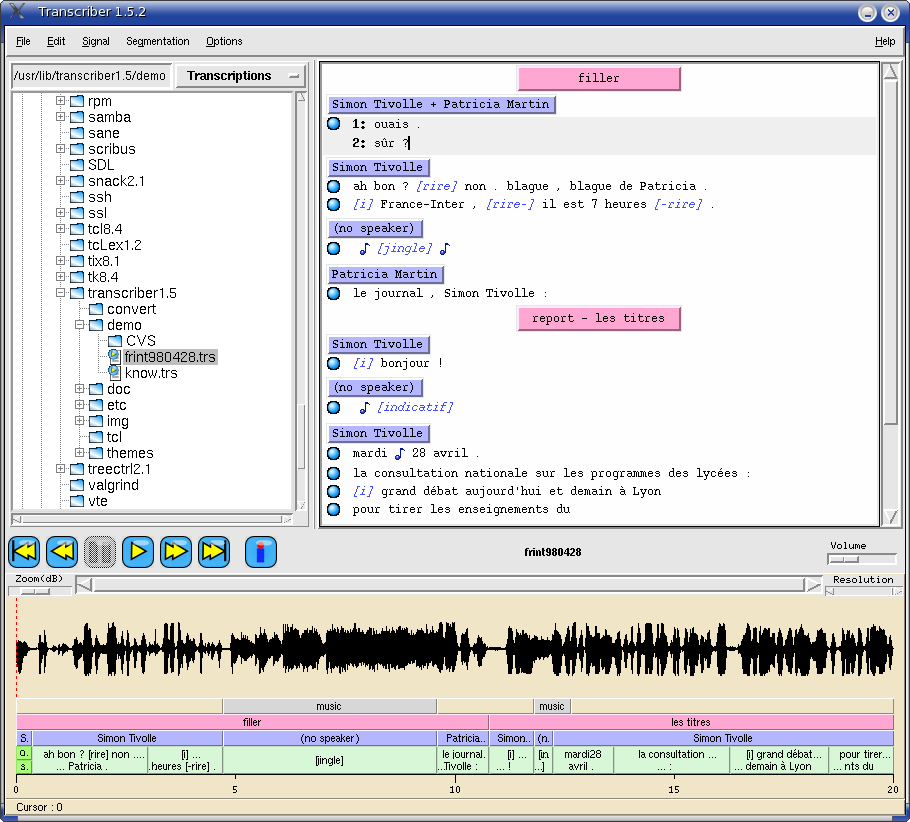
\includegraphics[scale=0.4]{rc/transcriber1.png}
\caption{Uživatelské rozhraní Transcriberu}
\label{fig:transcriber1}
\end{figure}

Toto je jeden z~důvodů, proč zobrazuji přepis v~podstatě jako jeden zalomený
řádek.

\subsection{Problém s~rychlostí}

Na zobrazení přepisu byly kladeny tyto požadavky:
\begin{enumerate}
\item{
    Právě přehrávané slovo aby bylo zvýrazněno;
    \label{feats:item:curword}
}
\item{
    Manuálně přepsané segmenty aby byly jasně odlišené od automaticky
    přepsaných;
    \label{feats:item:manualdistinct}
}
\item{
    Označení neprázdné množiny znaků (krom mezery) myší aby spustilo editační
    mód pro označený text doplněný na celá slova;
    při úspěšném uložení změny, aby se tato vmísila do zobrazeného textu;
    \label{feats:item:selectable}
}
\item{
    Kliknutí na slovo aby o~něm vyvolalo zobrazení kontextových informací
    (toto zvu {\em ,,vybrané slovo''}, neb pojem {\em ,,označené slovo''} je již
    obsazen);
    \label{feats:item:clickable}
}
\item{
    Celý přepis aby byl viditelný najednou pro možnost vyhledávání;
    \label{feats:item:showall}
}
\item{
    Stránka aby byla responzivní.
    \label{feats:item:speed}
}
\end{enumerate}

Skloubit tyto požadavky je obtížnější, než by se mohlo zdát. Zejména
responzivita se těžko slučuje s~ostatními body. Proč?

Body~\ref{feats:item:curword} až~\ref{feats:item:clickable} volají po tom, aby
každé slovo bylo obaleno ve vlastním elementu.
Bod~\ref{feats:item:showall} a medián počtu slov v~nahrávce zvíci šesti tisíc
dává dohromady šest tisíc elementů \texttt{span} jen pro statické zobrazení
textu.

Může se zdát, že to není takový problém, ale ovlivňuje to responzivitu a
paměťovou náročnost stránky.

V~původní, první verzi webové aplikace, jsem toto vyřešil obětováním
bodu~ref{feats:item:showall}: zobrazovaly se jen tři řádky textu, přičemž právě
přehrávané slovo se vždy drželo v~tom prostředním. Ukazuje to
obrázek~\ref{fig:makonfm} jen s~tím, že právě přehrávané slovo je v~prvním
řádku, poněvadž se přehrává začátek nahrávky. Díky pokroku ve webových
standardech a jejich podpoře ze strany prohlížečů je nyní možné řešení.

\begin{figure}[htpb]
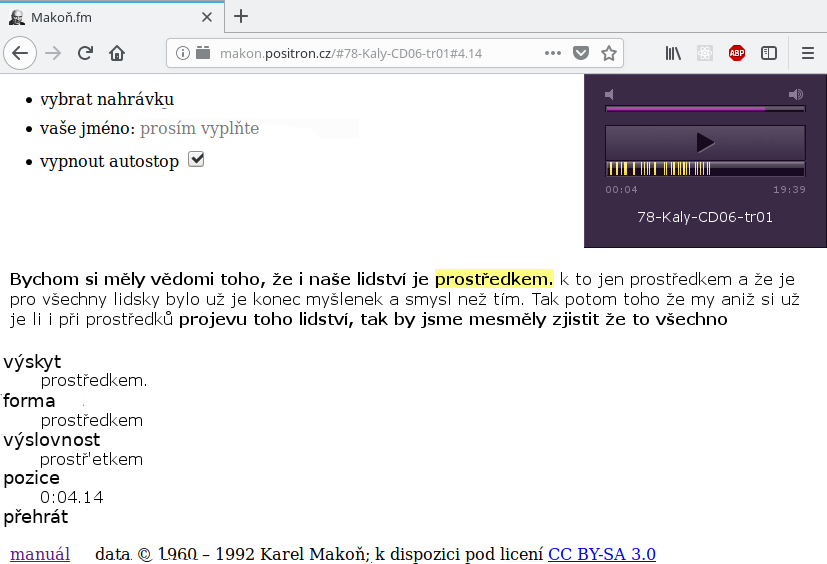
\includegraphics[scale=0.7]{rc/makonfm-cs-1.png}
\caption{Původní webové rozhraní z~roku 2012}
\label{fig:makonfm}
\end{figure}

\subsection{Řešení}

Můžeme využít šťastného faktu, že ručně přepsaná slova a automaticky přepsaná
slova mají tendenci se shlukovat. Průměrný počet slov v~jednom příspěvku je 7,9.
Navíc drtivá většina takových segmentů bezprostředně navazuje na další ručně
přepsané segmenty.\footnote{Medián počtu shluků je 1 (většina nahrávek nemá
žádné ručně přepsané slovo), maximum je 1109. Medián pouze z~nahrávek, které
obsahují ruční korekce, je 8.}
Z~toho plyne, že obalení každého souvislého shluku manuálně či automaticky
přepsaných slov do zvláštního HTML elementu nepředstavuje problém, což řeší
bod~\ref{feats:item:manualdistinct}.

Bod~\ref{feats:item:selectable} lze implementovat s~použitím metody objektového
modelu dokumentu ({\em DOM}) \texttt{document.selection} a objektů
\texttt{Range}, které umožňují nalézt nejhlubší HTML elementy a pozice v~jejich
textu, kde začíná a končí označený úsek. Díky tomu, že délka slov je známa, mohu
z~označeného úseku dovodit odpovídající slova v~přepisu.

Body~\ref{feats:item:curword} a~\ref{feats:item:clickable} se dá implementovat
dvěma způsoby: Buďto zabalením přehrávaného a vybraného slova do zvláštního
elementu anebo vykreslením zvýrazňujícího obdélníku na pozadí slova.

Výhodou obalení slov elementem by byla větší robustnost a menší náchylnost
k~chybám. Nicméně neustálé změny v~DOMu při přehrávání s~potenciálními častými
operacemi {\em reflow}\footnote{Při operaci reflow prohlížeč přepočítává pozice
všech elementů a překresluje je.} hovoří proti tomuto řešení. Nalézt přesné
pozice slova a vykreslení obdélníku přesně pod ním\footnote{Pod ním na ose Z.
Přes něho na osách X, Y.}, vyhnout se chybám v~pozicování a udržet
obdélník na správném místě i po změně velikosti okna či odskrolování, to je
dozajista výzva, nicméně přesto jsem zvolil tuto cestu. Navýšení výkonnosti pro
běžné používání převažuje potenciální chyby v~okrajových případech, najmě když
eventuální chyby nejsou kritické a zmizí při dalším přehrávání.

\section{Prototyp}

Webové rozhraní, umožňující přístup zájemcům k~nahrávkám a jejich přepisu, bylo
od začátku plánovanou součástí projektu. Rozhraní bylo navrženo s~těmito
požadovanými vlastnosmi:

\begin{itemize}
\item{výběr nahrávky ze~seznamu,}
\item{poslech nahrávky s~obvyklými ovládacími prvky přehrávače,}
\item{zobrazení přepisu nahrávky,}
\item{vyznačení právě přehrávaného slova,}
\item{možnost provést změnu v~přepisu,}
\item{automatické zarovnání přepisu se~zvukem,}
\item{případné odmítnutí přepisu, pokud zarovnání selže (přepis neodpovídá
vyřčeným slovům).}
\end{itemize}

První implementace byla založena na přehrávači \textit{jPlayer}, modulu pro
knihovnu \textit{jQuery}, který využívá standard HTML5 s~jeho elementem
\texttt{<audio>} a technologii \textit{Adobe Flash}. Pro~dynamickou odezvu
zobrazených prvků na~změny v~datovém modelu jsem použil knihovnu
\textit{knockout}.

Aplikace měla formu jediné stránky s~rozbalovatelným výběrem nahrávky,
ovládacími prvky přehrávače a třemi řádky přepisu. Při označení části
zobrazeného přepisu se stránka překryla rozhraním pro opravu přepisu, jež zvu
\textit{editačním okénkem}. V~editačním okénku se zobrazilo vstupní pole
(\texttt{<textarea>}) s předvyplněným současným přepisem, ovládací prvky pro
přehrátí odpovídající pasáže, odeslání opraveného přepisu a opuštění editačního
okénka.

Šlo o~prostou statickou HTML stránku s~JavaScriptem. K~audiu se přistupovalo
pomocí externí CDN, zatímco přepisy a API pro~zarovnávání oprav byly
na~zvláštním serveru.

Přepis byl uložen a přenášen ve~formátu \textit{JSONp}\footnote{JSON =
JavaScript Object Notation, JSONp = JSON with Padding}, čili jako \textit{JSON}
obalený v~javascriptové funkci kvůli zamezení problémů s~přístupem napříč
doménami.

%Každé slovo s~sebou neslo informaci o~svojí pozici v~nahrávce
%s~přesností na~setiny sekundy, výslovnost, zápis, slovníkovou formu, délku ticha
%za~slovem, informaci o~tom, zda bylo manuálně přepsáno nebo automaticky
%rozpoznáno, a v~případě automaticky rozpoznaných slov \textit{confidence
%measure} čili míru jistoty rozpoznání.

%Převod ze~zápisu slova do~jeho fonetické podoby se děje na~základě pravidlového
%algoritmu z~dílny Doc. Pavla Ircinga po~úpravě od~Mgr.~Nina Peterka, Ph.D. Tento
%algoritmus zahrnuje časté výjimky z~českých výslovnostních pravidel, ale
%neobsahuje rozsáhlý výslovnostní slovník cizích slov. Karel Makoň navíc nezřídka
%hovoří o~osobách, jejichž jména se v~mnoha korpusech neobjeví vůbec.

Nad rámec výše popsaných funkcionalit přibyly další na~základě přání uživatelů a
autorovy potřeby:

\begin{itemize}
\item{indikace, do~jaké míry je která nahrávka
přepsána\footnote{\label{fn:not-in-v2}Tato
funkcionalita momentálně není implementována v~nové verzi aplikace.},}
\item{manuální posouvání hranic přepisovaného zvukového
úseku\footnotemark[\getrefnumber{fn:not-in-v2}],}
\item{úprava zápisu slova s~ponecháním výslovnosti,}
\item{identifikace uživatelů včetně sezení, prohlížeče atp.,}
\item{vyhledávání v~přepisech.}
\end{itemize}

Tato původní verze posloužila k~přepsání asi 600 tisíc slov a běžela asi 5 let,
než bylo nutné ji nahradit.

\section{Verze 2}

Pro kompletní přepis aplikace se postupně objevilo několik důvodů. Hlavním
z~nich bylo, že původní aplikace mohla jen těžko sloužit pro širokou veřejnost
jako prostředek k~popularizaci nahrávek. Dalším důvodem bylo, že některé kýžené
funkce nebylo možné zprovoznit bez zásadních změn v~provedení. Především šlo
o~ekvalizér, čili frekvenční korekci při poslechu. Akutním důvodem pak byl fakt,
že všechny významné prohlížeče opouštěly podporu Flashe.

Pro novou verzi jsem zvolil technologie React + Redux\cite{abramov2015redux} jako aplikační rámec, Web
Audio API\cite{adenot2013web} jako platformu pro nakládání se~zvukem a Twitter Bootstrap jako základ
pro vzhled prvků. Zdrojový kód píšu v~ECMAScript~6 a o~kompilaci se stará
webpack.

\subsection{Výběr nahrávky}

První verze obsahovala všudypřítomný rozklikávatelný kategorizovaný seznam
nahrávek. Toto jednoduché řešení mělo jen málo nevýhod. Jedna z~nich byla, že
nešlo použít běžné textové vyhledávání. V~nové verzi je proto použit
dvousloupcový formát, kde vlevo je rozbalovací seznam kategorií a vpravo
lineární seznam nahrávek. Jednotlivé kategorie jsou pak skrolovacími odkazy
do~pravého sloupce a podle stupně skrolování se příslušná kategorie sama
rozbalí (tzv. scrollspy).

Pro lepší přehlednost a v souladu s principem Separation of Concerns je seznam
nahrávek pouze na~úvodní stránce a nikoliv všude.

\subsection{Zobrazení přepisu}

V~první verzi se zobrazovaly vždy tři řádky, kde v~prostředním bylo aktuálně
přehrávané slovo. Výjimkou samozřejmě byly případy, kdy se přehrával začátek
nebo konec nahrávky. Délka řádku odpovídala šířce okna prohlížeče. Takto malý
rozsah zobrazeného textu byl zvolen proto, že aby bylo možné vizuálně odlišit
ručně přepsaná slova od~automaticky rozpoznaných a od~nich ještě slovo aktuálně
přehrávané, muselo být každé slovo obaleno ve~vlastním HTML elementu. Při~větším
množství slov pak bylo rozhraní velice náročné na~výpočetní výkon a znatelně
pomalé, což při synchronním zobrazování přepisu s~přehráváním zvuku není
přijatelné.

Zobrazení jen tří řádků mělo pochopitelně velké nevýhody. Především to, že se
člověk nemohl zorientovat v~širším rámci nahrávky (jejíž průměrná délka je kolem
hodiny) a že opět nebylo možné vyhledávat v~jejím rámci. Výhodou naopak bylo, že
aktuálně přehrávané slovo bylo vždy snadné najít. Nemožnost označit a tedy ani
přepsat příliš dlouhý úsek bylo pro uživatele možná někdy nepříjemné, ale
redukovalo chyby jak v~přepisu, tak v~automatickém zarovnávání.

Čtvero elementů, které je potřeba graficky odlišit, je: 
\begin{enumerate}
\item{automaticky přepsaná slova},
\item{manuálně přepsaná slova,}
\item{slovo aktuálně přehrávané,}
\item{slovo vybrané kliknutím.}
\end{enumerate}

Zobrazení celého přepisu při zachování plynulosti a grafickém odlišení
čtvera elementů bylo první velkou výzvou pro návrh stránky přehrávání.
První, nezaslouženou pomocí k~tomu byl vývoj výkonu počítačů od~vzniku první
verze, jakož i optimalizace prohlížečů na~rychlost. Množství elementů, které lze
nyní realisticky zobrazit, se znatelně zvýšilo, ačkoliv naivní řešení zabalení
každého slova stále není praktické. Druhým pomocným faktorem je, že manuálně a
automaticky přepsaná slova se většinou vyskytují ve~větších shlucích. Jen
v~málokterých souborech se často střídají manuálně a automaticky přepsané úseky.
To vypovídá o~nevoli uživatelů k~jinému než kompletnímu, lineárnímu přepisu.
% TODO: ref. aktivní učení
Každý shluk manuálně respektive automaticky přepsaných slov stačí tedy zabalit
do~jednoho elementu.

Zvýraznění jednotlivých slov -- aktuálně přehrávaného a vybraného klikem myší --
se realizuje pomocí umístění barevného rámečku pod~zvýrazněné slovo. To lze
provést díky tomu, že prohlížeče nyní umožňují zjistit polohu označeného textu a
označení lze provést automaticky.\footnote{Viz \texttt{getClientRects} a
\texttt{Range} ve~webových standardech.}

\subsection{Web Audio API}

Přechod na~tuto technologii umožnil některé pokročilé funkce, avšak za~relativně
vysokou cenu. Web Audio API je standard pro~pokročilé zpracování zvukového
signálu v~prohlížeči. Základním konceptem je graf procesních uzlů, které mají
vstup a výstup a mohou se libovolně propojovat. K~dispozici jsou zdroje zvuku
jako oscilátory nebo přehrávače streamů, souborů (tag \texttt{<audio>}) a dat
v~paměti (\texttt{AudioBuffer}) a efekty jako zesílení, dynamická komprese, či
mixování kanálů.

Velká výhoda Web Audio API oproti elementu \texttt{<audio>} je možnost přesného
časování, až na~jednotlivé samply. Přehrávání výseku odpovídajícího označenému
textu se proto nemusí provádět pomocí velice nepřesného časovače
\texttt{setTimeout}.

Bez~Web Audio API by také nebylo možné provádět frekvenční korekci při poslechu,
čili mít tzv. \textit{ekvalizér}. Ten je zapotřebí, protože některé nahrávky
mají v~určitém frekvenčním pásmu silný šum, jehož odstranění je s~ekvalizérem
snadné a komfort poslechu se tak razantně zvýší.

Další funkcí, kterou Web Audio API umožňuje, je stahování úseků. Označením
přepsaného textu se definuje úsek nahrávky a ten je možné uložit bez~dalšího
síťového přenosu. Tato funkce však vyžaduje, aby nahrávka byla dekódovaná
v~paměti. Vzhledem k~tomu, že nahrávky mají běžně i hodinu a půl, trvá její
stažení a dekódování opravdu dlouho a navíc prohlížeč kvůli tomu spotřebuje přes
gigabyte operační paměti.

Jsou plány na~to, aby Web Audio API umožnila dekódovat jen část
nahrávky,\footnote{github.com/WebAudio/web-audio-api/issues/1305}, avšak
palčivost problému mne přiměla nečekat, viz následující sekci.

Díky tomu, že Web Audio API umožňuje přehrávání binárních dat z~proměnné
v~paměti, nabízí se dekódovanou nahrávku uložit na~persistentní úložiště
uživatelova počítače a při opětovné návštěvě stránky data místo stahování odsud
nahrát.

Moderní prohlížeče poskytují několik bran k~úložišti na~místním disku.
Nejtradičnějšími jsou bezesporu \textit{cookies}, které jsou však pro ukládání
objemnějších dat zcela nepoužitelné. Velice slibnou se jeví
\textit{localStorage}, umožňující ukládání párů klíč-hodnota. I zde však
narážíme na~příliš omezující kvóty. Kupříkladu Firefox ji má na 10MB, přičemž
potřeba je asi 1GB. Dalším kandidátem je \textit{File System API}. Tento
standard pro~izolovaný souborový systém k~dispozici webové aplikaci je zcela
ideálním řešením -- dá se zde i explicitně požádat o~konkrétní diskovou kvótu a
uživatel tak má volbu bez nutnosti práce programátora webové aplikace. Kamenem
úrazu je zde však podpora, která se momentálně omezuje pouze na Google Chrome.

Existuje ještě standard \textit{IndexedDB API}, který má uspokojivou
podporu a uložení gigabytu dat je s~ním možné, byť ne zaručené. S~využitím
abstrahující knihovny \textit{Dexie} jsem proto skrz tento standard ukládání
implementoval. Pro uživatele, kteří delší dobu pracují na jedné a téže nahrávce
se tím přináší velká úspora času a přenesených dat. Nicméně s~rozdělením
nahrávek na segmenty přestala být potřeba ukládat nahrávky aktuální.

\section{Rozdělení nahrávek na úseky}

Vzhledem k~tomu, že ani v~roce 2019 není kurzorový přístup ke zvukovým datům
skrze Web Audio API v~dohlednu, a k tomu jak odrazující dopad má nutnost
stahovat a dekódovat celou nahrávku aspoň při jejím prvním načtení, nezbylo mi,
než změnit způsob, jakým jsou nahrávky uloženy.

Nahrávky jsou uloženy v~několika instancích pro různé účely:

\begin{enumerate}
\item{na backendovém serveru ve formátu MFCC pro nucené zarovnávání,}
\item{v~repozitáři LINDAT ve formátu FLAC za účelem archivace a bádání,}
\item{na CDN ve formátu mp3 za účelem přímého stažení uživatelem,}
\item{taktéž na CDN ve formátech OGG/Vorbis a mp3 pro webové rozhraní.}
\end{enumerate}

Pouze poslední jmenovanou instanci je žádoucí ukládat tak, aby každý soubor byl
jen tak velký, aby jeho stažení a dekódování trvalo únosně dlouho. V~ostatních
případech je lépe zachovat uložení, kde jedna nahrávka odpovídající většinou
jedné straně kazety či jednomu průchodu pásky z~kotouč na kotouč. Třetí a čtvrtá
instance však navzdory rozdílnému účelu sdílejí tatáž data. Bylo proto nutné je
duplikovat.

\subsection{Délka segmentů}

Délka úseků, na které nahrávky rozděluji, ovlivňuje, jak dlouho se každý segment
bude stahovat a dekódovat.
Délka úseků, na které nahrávky rozděluji, ovlivňuje, jak dlouho se každý segment
bude stahovat a dekódovat.  Čas stahování a dekódování segmentu, který obsahuje
slovo, na němž je kurzor při prvním požadavku o~přehrávání, je roven zpoždění od
uživatelské akce k začátku přehrávání. Podle internetového periodika
UXMovement\cite{foursecondrule}, začíná uživatel po čtyřech sekundách čekání
upouštět od předchozího záměru. Podle článku Nielsen Norman
Group\cite{websiteresponsetimes} je hranice únosnosti 10 sekund.

Pokud budou úseky příliš dlouhé, jejich stahování a dekódování zabere příliš
mnoho času. Na druhou stranu s každým předělem vnášíme do přehrávání bod, kde se
úseky nalepují a může tam vyvstat artefakt. Také s~každým segmentem se pojí
extra HTTP request s~nezanedbatelnou režií.

Jako vhodný kompromis se jeví segmenty o délce 30 - 120 sekund. Velikost
dvouminutového segmentu je v~komprimovaném formátu při mono/24KHz kolem 0.6MB a
na Intel Core2 o 2,5GHz se dekóduje asi 1.6 sekundy.

\subsection{Metody hledání bodů předělu}

Vhodným výběrem bodů předělu můžeme omezit dopad případných artefaktů
způsobených nepřesným navázáním. Ideálním by bylo dělit nahrávky v~momentech
ticha. Ne vždy jsou momenty ticha každé dvě minuty, proto z momentů ticha
ustupme k~požadavku pauzy v~řeči. Hovořit dvě minuty bez nádechu hraničí
s~nemožností. Potýkáme se tedy s~úlohou nalézt pauzy v~řeči. Jednak je třeba
ujasnit, podle jakého klíče budeme pauzy vybírat, a jednak, jak je budeme přesně
hledat.

Hledat pauzy v~řeči lze různými způsoby. Nejspolehlivější a nejnáročnější je
manuální označování pauz. Pokoušel jsem se o~to sám a dosáhl jsem rychlosti
přibližně čtyřnásobku rychlosti přehrávání, tedy jeden zapsaný bod předělu za
třicet sekund.

Další velice spolehlivou metodou je hledání podle predikovaných pseudofonémů
ticha v~zarovnaném přepisu. Tuto metodu jsem mohl namnoze použít, neboť
k~většině nahrávek mám automatický nebo i manuální přepis.

Tam, kde pořízení přepisu nebo jeho automatické zarovnání selhalo, lze použít
detekci ticha prostou akustickou analýzou. Tato metoda je velice náchylná
k~chybám v~případě nahrávek s~malým poměrem signálu k~šumu, kterých se v~korpusu
Karla Makoně vyskytuje neutěšeně mnoho.

Kde nepomůže ani metoda detekce ticha, což se pozná podle toho, že detekované
pauzy jsou příliš daleko od sebe nebo naopak zabírají valnou část nahrávky,
nezbývá, než určit body předělu ve fixních intervalech, nehledě na to, že jich
většina padne doprostřed slova.

Pokusy dvě metody vyloučily: Manuální hledání bylo příliš neefektivní. Kromě mne
se dalších asi pět dobrovolných anotátorů o~tento úkol pokusilo a došla jim
trpělivost po nule až deseti minutách označkovaného materiálu. Detekci pomocí
zarovnaného přepisu šlo použít i na některé nahrávky, u nichž přepis selhal tím
způsobem, že se rozdělily na menší části, přepsaly se ony -- zpravidla
s~katastrofální úspěšností. Tento přepis opět v~některých případech selhal, ale
většina takové nahrávky byla nějakým přepisem pokryta. A jakkoliv nekvalitní
takový přepis byl, právě dlouhé mezery mezi slovy se nalezly s~uspokojivou
přesností. Krátké úseky, na nichž selhalo rozpoznávání řeči, byly pak příliš
obtížné i pro detekci pomocí ticha. Jednalo se o úseky bez řečových událostí,
nebo s~extrémním šumem.


Celkový počet různě získaných bodů předělu shrnuje
tabulka~\ref{tab:splitpoints}\footnote{Vysoký počet předělů fixní délkou je způsoben tím, že
k~některým nahrávkám jsem doposud nepořídil zarovnaný přepis s~vyznačením délky
ticha.}.

\begin{table}[htpb]
\begin{center}
\begin{tabular}{|l|l|}
\hline
metoda získání & počet použitých \\
\hline
manuálně & 0 \\
podle zarovnaného přepisu & 60424 \\
podle detekce ticha & 0 \\
fixní délkou & 22043 \\
celkem & 82467 \\
\hline
\end{tabular}
\caption{počet bodů předělu podle metody jejich získání}\label{tab:splitpoints}
\end{center}
\end{table}

\subsection{Výběr bodů předělu}

V~naivní metodě určování bodů předělu pomocí fixního intervalu jsem zvolil délku
šedesáti sekund. Že to je délka přijatelná, se diskutuje výše a s~další
optimalizací tohoto parametru jsem neztrácel čas.

Zajímavější je situace u~hledání pomocí zarovnaného přepisu. Zde se jedná
o~programátorský úkol, kde na vstupu máme posloupnost slov vyskytujících se
v~přepisu nahrávky, z~nichž každé s~sebou krom své formy a výslovnosti nese
informaci, kde začíná, a pokud obsahuje na konci ticho, pak kde začíná
pseudofoném ticha a jak je dlouhý.  Redukovat tedy vstup můžeme na posloupnost
párů čísel, kde první vždy udává počátek ticha a druhé jeho konec. Na výstupu
očekáváme posloupnost časových pozic, které rozdělují nahrávku na úseky o~délce
nejméně 30 sekund, nejvýše 120 sekund, a které jsou uprostřed co nejdelších
segmentů ticha.

Povšimněme si, že úloha nemá řešení, pokud je nahrávka kratší třiceti sekund. To
ovšem jednak v~mluveném korpusu Karla Makoně nenastává a jednak by to nevadilo,
proože takovou nahrávku bychom jednoduše nechali v~jednom souboru.

Druhým případem, kdy úloha nemá řešení, je, když mezi dvěma sousedními pauzami
je rozestup větší než 120 sekund. Takový případ nastává, když je samotné
detekované ticho velmi dlouhé. Takové případy jsem řešil manuální úpravou.

Hledaný algoritmus se zdá být typickým příkladem pro dynamické programování:
Nalezneme ideální rozdělení nahrávky, která obsahuje jen první slovo, a poté
přidáváme slova a na základě dosavadního řešení a nového slova řešení
rozšiřujeme.

Je ale i jednodušší varianta: Začneme s~množinou všech pauz a iterujeme přes ně
od nejkratší po nejdelší. Pauzu z~množiny odebereme, pokud sloučením sousedních
segmentů nevznikne segment delší než 60 sekund. Přes vybrané pauzy znova
iterujeme a pauzu odebereme, jestliže jeden z~jejích sousedů má méně než 30
sekund.

Zbylá množina pauz splňuje počáteční podmínky, pokud to je vzhledem ke vstupním
datům možné. Algoritmus je nejen jednoduchý na naprogramování, ale má také milou
lineární složitost.

\subsection{Pojmenování souborů}

Jsou-li vybrány body předělu, mohou se nahrávky podle nich rozdělit a výsledné
segmenty uložit na disk. Zde vyvstává otázka, jak rozdělit soubory do adresářů a
jak je pojmenovat. Že způsob uložení souborů hraje roli, dokládá i Reppen (2010)\cite{reppen2010building}. Zvolil jsem tento formát:

\texttt{{\em{}ID}/{\em{}format}/{\em{}ID}--from-{\em{}ZACATEK}--to-{\em{}KONEC}.{\em{}PRIPONA}}

tedy například

\texttt{88-04A/ogg/88-04A--from-1155.27--to-1211.53.ogg}.

Důvody jsou tyto: Není praktické z~důvodu omezení mnoha souborových systémů mít
příliš mnoho souborů v~jednom adresáři. Proto rozdělení do adresářů podle
identifikátorů nahrávek. Že formát je právě podadresář identifikátoru a ne třeba
nadadresář, je arbitrární, obojí by bylo možné, nebo i mít soubory všech formátů
v~jednom adresáři a jen je odlišovat příponou.

Zopakovat identifikátor nahrávky i v~názvu souboru jsem se rozhodl proto, aby
případný zatoulaný soubor mohl být snáze identifikován. Díky tomu, že se do
názvu souboru uvede začátek i konec úseku v~rámci nahrávky zajistí, že název
souboru přesně popisuje jeho obsah. Oproti tomu např. lineární číslování by při
změně bodů předělu vedlo k~tomu, že jeden název souboru by byl totožný pro různé
úseky v~různých verzích korpusu. To by mohlo vést k~problémům s~cachováním.
Identifikátory pomocí kontrolních součtů nebo jinak postavených na základě
binárního obsahu souboru by vedlo k~nutnosti změnit identifikátory při každé
změně komprese apod., ačkoliv slyšitelný rozdíl by třeba nebyl žádný.

Nyní, pokud by došlo ke změně bodů předělu, by se nové i staré úseky musely
uchovávat v~jednom adresáři a, až by všechny instance starých úseků byly
vyhlazeny z~paměti cache všech klientů, by se staré mohly smazat. Jedinou
nevýhodou je, že by se musely nové přebrat od starých, ale to není problém.

\subsection{Překryv úseků}

Při testování se ukázalo, že vyřízneme-li pomocí programu \texttt{sox} úsek
zvukového souboru, výsledný soubor skončí přehrávání o~několik desetin sekundy
dříve. Jako by chybělo posledních několik set samplů. Příčinu tohoto fenoménu
zatím neznám. Kompenzoval jsem jej tím, že jsem každý úsek prodloužil o~půl
sekundy. Následkem toho bylo potřeba upravit přehrávání tak, aby každý úsek
skončil tehdy, až dohraje jeho metadaty daná délka, nikoliv až do skutečného
vyčerpání zvukových dat.


\section{Použití aplikace}

Aplikace {\em znamená} použití. Použitelnost je tedy klíčovým faktorem pro její hodnocení.

\subsection{Expertíza uživatelů}

Přepis, který pořizuji, je na hranici toho, co se dá nazvat lingvistickou
anotací dat. V~naší požehnané části světa, kde podíl analfabetů je zanedbatelný,
je přepis mluveného slova stěží odbornou prací. Na druhou stranu zajistit, aby
přepis přesně odpovídal mluvenému projevu
\begin{itemize}
\item{jakožto vyjádření vyřčených slov a jejich významu,}
\item{na fonetické úrovni foném na foném}
\item{a na časové ose}
\end{itemize}
je za hranicemi toho, co se dá očekávat od nevyškoleného uživatele.

Lingvistická anotace dat obecně vyžaduje zaškolené pracovníky. Podíváme-li se
např. na Pražský závislostní korpus, můžeme si povšimnout, že od anotátorů
vzešla taková úroveň expertízy, že se stali spoluautory\cite{hajivc2005complex}.

Crowdsourcing, přístup založený na komunitní spolupráci nebo zapojování
dobrovolníků nabývá na popularitě při získávání hodnot, které by jinak byly
neúnosně drahé, viz podsekci~\ref{ssec:setting-corpora}. Nicméně např. Maekawa (2000)\cite{maekawa2000spontaneous} popisuje tvorbu
mluveného korpusu spontánní japonštiny s~využitím placených anotátorů.

Ve většině případů je kvalita pro anotaci dat velmi důležitá, proto je aspoň
nějaká kontrola nezbytná, ať už je odbornost anotátorů jakkoliv vysoká. Je
zřejmé, že čím méně expertízy na straně anotátorů, tím silnější kontroly je
zapotřebí.

Běžnou metodou kontroly kvality je mezianotátorská shoda. To má obrovskou
nevýhodu, že každá část dat musí být anotována aspoň dvakrát, což snižuje
výtěžnost aspoň o 50\%.

Ještě jeden důvod hovoří proti jejímu použití v~případě tohoto projektu. Webová
aplikace je dělaná pro lidi, kteří chtějí poslouchat Makoňovy nahrávky
z~vlastního zájmu a jejich přínos pro kvalitu přepisu je spíše vedlejším
produktem. Nebylo by snadné přesvědčit je, aby si vybrali právě nahrávku, kterou
už někdo jiný přepsal.

Naštěstí lze implementovat automatický mechanismus, který uživatelům dopomůže
k~vyšší kvalitě příspěvků.

Webová aplikace vychází z~předpokladu, že a-priori existuje nějaký přepis ke
každé nahrávce, takže uživatelův příspěvek je vlastně korekcí. Každý příspěvek
má formu nahrazení textového segmentu jiným. Jelikož přepisy jsou zarovnány
s~audiem na časové ose, víme také, jakému přesně úseku nahrávky daný text
odpovídá.

Dále se vychází z~existence akustického modelu pro nahrávky, viz kapitolu~\ref{kap:asr}.

Díky těmto dvěma prvkům mohu provést nucené zarovnání (forced alignment) textového úseku
s~audiem. V~případě selhání zarovnání můžeme předpokládat, že úsek byl přepsán
chybně, příspěvek odmítnout a dát tím uživateli zpětnou vazbu. Jelikož
jednotlivé úseky odpovídají akustickému modelu v~různé míře, dochází k~falešně
pozitivním i negativním vyhodnocením.

Falešně pozitivní případ (když systém přijme chybný přepis) představuje skutečný
problém, protože chyba vstoupí do trénovacích dat. Falešně negativní případy
mohou uživatelé často obejít tím, že správný, leč odmítnutý přepis, pošlou
znova, rozdělený do kratších částí. Touto metodou by se pochopitelně mohlo také
podařit vnutit systému nesprávný přepis. Nepředpokládám však na straně uživatelů
zlou vůli.

Krom zachycení chybného přepisu slouží nucené zarovnání k~přesné synchronizaci
na časové ose. Tento prvek zcela chybí prakticky ve všech programech pro přepis.
Ku příkladu Transcriber očekává časové zarovnávání na úrovni
frází ze strany uživatele. Transcribe
nechává uživatele přidat časové značky
kamkoliv do textu. Není zde žádný akustický model, tedy nic, vůči čemu provádět
zarovnání.

\subsection{Pořízení fonetického přepisu}
\label{ssec:porizeni-fonetickeho-prepisu}

Fonetický přepis je nezbytný pro trénování akustického modelu. Pořizuje se
provedením nuceného zarovnání na každý {\em ortograficky} manuálně přepsaný segment. Pokud je více
výslovnostních variant, automaticky se zvolí ta, která lépe odpovídá akustickému
modelu. Na to je potřeba pořídit výslovnostní varianty každého slova. Používám
kombinaci pravidlového převodníku inspirovaého Psutkou et
al. (2004)\cite{psutka2004development} a dynamického výslovnostního slovníku. Dynamický
výslovnostní slovník je seznam alternativních výslovností každého slova, který
se rozšiřuje s~používáním aplikace.

Manuál k~aplikaci vyzývá uživatele, aby text přepisovali podle standardního
českého pravopisu, ale při zachování maximální věrnosti vyřčených slov, tedy aby
nekorigovali \fontspec{DoulosSIL} /ɲaːk/ \normalfont na {\em nějak}, nýbrž
přepsali doslova jako {\em ňák}. Fonetický slovník obsahuje časté výslovnostní
varianty, např. počáteční \fontspec{DoulosSIL} /v/ \normalfont ve slovech
začínajících na \fontspec{DoulosSIL} /o/\normalfont {\em (vopice vobludná)}.

V~případě slov s~nestandardní výslovností, tedy primárně cizích slov, se od
uživatelů žádá, aby slovo přepsali foneticky. Teprve po úspěšném zarovnání a
integrace do přepisu mohou slovu nastavit kýženou pravopisnou formu. Toto je
jeden z~mála případů, kdy se od uživatele chce něco nekonvenčního.

Když je pravopisně chybný, fonetický zápis poslán, pak pokud projde fází
nuceného zarovnání, se integruje do zobrazeného přepisu. Datová reprezentace
každého slova sestává z~těchto prvků:
\begin{enumerate}
\item{Výskyt:
    slovo, jak se vyskytuje v textu, včetně zachování velkých a malých písmen a
    přilehlé interpunkce.
}
\item{Slovní forma:
    slovo, jak je zaneseno v~jazykovém modelu a ve výslovnostním slovníku.
    (Slovní forma se odvozuje algoritmicky z~výskytu převedením do malých písmen
    a odstraněním neabecedních znaků. Z~toho plyne, že interpunkce a všechny
    neabecední znaky jsou vždy součástí přilehlého slova a nikdy netvoří token
    samy o sobě.)
}
\item{Výslovnost:
    seznam fonémů.
}
\item{Časová značka:
    vzdálenost počátku slova od počátku nahrávky v~sekundách s~přesností na dvě
    desetinná místa.
}
\item{Manuálně přepsané:
    pravdivostní hodnota odlišující manuálně přepsaná slova od automaticky
    přepsaných.
}
\item{Confidence measure:
    míra jistoty, se kterou bylo slovo predikováno, pouze u automaticky
    přepsaných slov.
}
\item{Ticho:
    začátek a délka ticha, pokud se za slovem vyskytuje.
}
\end{enumerate}
Jakmile je slovo součástí přepisu, lze upravit jeho {\em výskyt}, tedy jak se
jeví v~textu. Nyní může uživatel vložit správnou ortografickou formu odchylující
se od českých pravidel výslovnosti.

To má za následek přidání dvojice {\em slovní forma - výslovnost} do dynamického
výslovnostního slovníku. Tento úkon je proto nutné provést jen jednou pro každé
slovo. Pokaždé, když na toto slovo libovolný uživatel narazí znova, stačí zadat jeho
ortografickou formu a správná výslovnost se dovodí automaticky.

\subsection{Fonetický zápis}
\label{ssec:respelling}

Přese všechny výhody reprezentace fonémů podle systému PACal se nejedná o
pratktický zápis výslovnosti pro laické Čechy. Díky jednoduchému, povětšinou
deterministickému mapování mezi fonémy a grafémy je fonetický zápis, nebo jak
se tento mechanismus označuje anglicky, {\em pronunciation respelling},
v~češtině něčím přirozeným a spolehlivým. Není ani potřeba explicitního dělení
slabik, jako tomu je u angličtiny
(Wikipedie\footnote{https://en.wikipedia.org/wiki/Pronunciation\_respelling}
udává příklad {\em ``Diarrhoea'' is pronounced DYE-uh-REE-a}).
Že tato technika je přirozenou pro všechny rodilé mluvčí češtiny se základním vzděláním,
postuluji jako fakt bez podpůrného výzkumu a zakládám to čistě na vlastní
zkušenosti.

Převod z~fonetického zápisu do PACal obstarává zmíněný převodník, viz
podsekci~\ref{ssec:porizeni-fonetickeho-prepisu}. Je ale zapotřebí i opačného
směru, aby se uživateli mohla dát možnost zkontrolovat, zda slovo, které
přepsal, se uložilo se správnou výslovností.

Za tímto účelem jsem vytvořil javascriptový modul pro převod mezi seznamem
fonémů a českým fonetickým zápisem.

Algoritmus je jednoduchý. Ve většině případů jeden foném odpovídá jednoznačně
jednomu písmenu ve fonetickém přepisu. Výjimky jsou tyto:
\begin{enumerate}
\item{Foném \texttt{x} se píše {\em ch}.}
\item{Fonémy \texttt{dz, dzh} se píší {\em dz, dž}.}
\item{Dvojhlásky \texttt{aw, ew, ow} se píší {\em au, eu, ou}.}
\item{
    Sekvence \texttt{c h, o u, a u, e u, d z, d zh} se píší
    {\em c'h, o'u, a'u, e'u, d'z, d'ž}.
    Budiž však poznamenáno, že sekvence \texttt{c h} je ryze hypotetická, ana
    porušuje spodobu znělosti.
}
\item{
    Neznělou zvýšenou alveolární vibrantu označuji {\em ř'}.
}
\item{
    Palatální a labiodentální nazála se píší {\em n', m'}.
}
\item{Ticho na konci slova ve fonetickém přepise nevyznačuji.}
\end{enumerate}

Modul umožňuje obousměrný převod, ačkoliv v~aplikaci je zapotřebí jen směr ze seznamu fonémů do
fonetického zápisu určeného pro člověka. Uživatel sice může explicitně vyznačit
neznělé {\em eř} oproti znělému, či posloupnost hlásek {\em o}, {\em u} oproti
dvojhlásce {\em ou} pomocí apostrofu. Za sedm let provozu však tohoto nebylo ani
jednou potřeba.

Podotýkám, že ve výstupu převodníku do fonetického zápisu se nikdy nevyskytují
sekvence {\em di, ti, ni, dě, tě, ně}. Palatální souhlásky jsou vždy vyjádřeny
explicitně a např. sekvence {\em n i} se vždy vyjádří jako {\em ny}.

V tabulce~\ref{tab:priklady-fonetiky} uvádím několik příkadů slov, jejich výslovností a fonetickým zápisem, jak jej
produkuje algoritmus, pokud na vstup dostane příslušnou výslovnost ve formátu
PACal:

\begin{table}[htpb]
\fontspec{DoulosSIL}
\begin{center}
\begin{tabular}{|l|l|l|l|}
\hline
slovo & výslovnost v~IPA & výsl. v~PACal & fonetický zápis \\
\hline
nic & ɲit͡s  & nj i c & ňic \\
kdo & gdo & g d o & gdo \\
disk & disk & d i s k & dysk \\
dřít & dr̝iːt & d rzh ii t & dřít \\
třít & tr̝̊iːt & t rsh ii t & tř'ít \\
auto & aʊ̯to & aw t o & auto \\
nauka & nauka & n a u k a & na'uka \\
džbán & d͡ʒbaːn  & dzh b aa n & džbán \\
odžít & odʒiːt & o d dz ii t & od'žít \\
odznak & od͡znak  & o dz n a k & odznak \\
podzemí & podzɛmiː & p o d z e m ii & pod'zemí \\
noc & not͡s  & n o c & noc \\
tento & tɛnto & t e n t o & tento \\
hangár & ɦaŋgaːr & h a ng g aa r & han'gár \\
samba & samba & s a m b a & samba \\
tonfa & toɱfa & t o mg f a & tom'fa \\
\hline
\end{tabular}
\caption{Příklady algoritmicky získaného fonetického zápisu}\label{tab:priklady-fonetiky}
\end{center}
\end{table}
\normalfont

Použití apostrofu pro rozlišení víceznačností a zvláštností není stoprocentně
intuitivní a představuje další bod, kde je zapotřebí uživatele zaškolit, aby
tuto funkcionalitu dokázal patřičně využívat.

\subsection{Vyhodnocení kvality přepisů}

Jak stojí výše, webová aplikace krom jiného slouží pro získání kvalitního
zarovnaného přepisu od laických uživatelů. Pokusím se vyhodnotit, do jaké míry
se to podařilo.

Pro vyhodnocení kvality přepisů nemám žádná referenční data. Naopak, přepisy
používám jako gold standard, tedy referenční data pro trénování akustického ba i
jazykového modelu. Lze se však namátkou podívat na několik vzorků a získat tak
představu o tom, jak si systém vede.

Jednou z~věcí, které můžeme posoudit, jsou přijetí a odmítnutí příspěvků
zarovnávačem. Celkem z~109640 pokusů o zarovnání jich 3419 bylo odmítnuto, což
je 3.12\%. Manuálně jsem prošel 20 náhodně vybraných odmítnutých pokusů a
přišel jsem k~těmto číslům:
\begin{itemize}
\item{
    V~\textbf{11} případech se jednalo o falešné negativum, kde přepis byl
    správný a měl být přijat,
}
\item{
    ve \textbf{4} případech byly příčinou odmítnutí akustické nedostatky jako
    např. šum,
}
\item{
    ve \textbf{4} případech se jednalo o pravdivá negativa způsobená chybně
    zvolenými hranicemi segmentu a
}
\item{
     v \textbf{1} případě se jednalo o pravdivé negativum způsobené chybným
    přepisem.
}
\end{itemize}

Ve 25\% tohoto minimalistického vzorku tedy zarovnávač splnil svoje validační
poslání, předšed tomu, aby se do trénovacích dat dostal chybný vzorek. V~55\%
případů selhal a byl jen otravnou překážkou v~práci a ve zbývajících 20\%
případů sice odmítl validní přepis, ale zabránil tomu, aby se do trénovacích dat
dostal defektní vzorek, na což se dá dívat v~pozitivním světle.

Dá se také vyhodnotit scénář s~nestandardní výslovností. Za tím účelem jsem
z~dynamického výslovnostního slovníku vybral 4 nadějné záznamy a prohlédl si
příspěvky, které je obsahují. Tabulka~\ref{tab:eval-pronunc} uvádí pro každý
z~nich správnou ortografickou formu, chybnou výslovnost získanou převodníkem,
správnou výslovnost a konečně možný fonetický zápis. Ke každému údaji je uvedeno,
kolikrát se objevil v~manuálně přepsaných datech.

\begin{table*}[htpb]
\fontspec{DoulosSIL}
\begin{center}
\begin{tabular}{|l r|l r|l r|l r|}
\hline
psaná forma                     & \#
    & \makecell{chybná\\ výslovnost} & \#
        & \makecell{správná\\ počeštělá\\ výslovnost}  & \#
            & fonetický zápis               & \# \\
\hline
Moody & 2 & moʔodi & 0 & muːdi & 4 & múdy, můdy & 2 \\
Descartes & 2 & dɛst͡s artɛs  & 0 & dɛkaːrt & 4 & dekárt & 2   \\
Weinfurter & 30 & vɛinfʊrtɛr & 13 & vajnfʊrtr & 19 & vajnfurtr & 2 \\
Michelangelo & 6 & mixɛlaŋgɛlo & 2 & mikɛlaŋd͡ʒ ɛlo  & 4 & mikelandželo & 0 \\
\hline
\end{tabular}
\caption{Příklady nestandardní výslovnosti v~manuálních přepisech}
\label{tab:eval-pronunc}
\end{center}
\end{table*}

\begin{table*}[htpb]
\begin{center}
\begin{tabular}{|l|r|r|}
\hline
 & foneticky správně & foneticky chybně \\
\hline
ortograficky správně & 25 & 15 \\
\hline
ortograficky chybně & 6 & 0 \\
\hline
\end{tabular}
\caption{Správnost fonetické a ortografické reprezentece cizích slov na základě
tabulky~\ref{tab:eval-pronunc}}
\label{tab:pronunc-rate}
\end{center}
\normalfont
\end{table*}

Z~tabulky~\ref{tab:pronunc-rate} je patrno, že většina případů je správně jak
po stránce fonetické, tak po stránce pravopisné. Pouze asi ve 13\% případů je
uchována pravopisně nesprávná forma. To připisuji tomu, že uživatelé, kteří jsou
si této problematiky vědomi, většinou celý proces dokončí a formu upraví.

Na druhou stranu téměř třetina případů vykazuje ponechání chybné fonetické
reprezentace. To představuje závažný problém alespoň z~dvou úhlů pohledu: Jednak
se tím dokazuje, že nucené zarovnání selhává při zachycení zcela odlišné
výslovnosti, a jednak se touto cestou dostávají do trénovacích dat špatné
vzorky.

Jednou z~patrných příčin je, že dynamický slovník rozpoznává pouze exaktně
shodná slova. V~jednom souboru je například vidět, jak všechny výskyty slova
{\em Weinfurter} mají výslovnost správně, zatímco ostatní formy, jako např. {\em
Weinfurterovi}, chybně.

Krom toho jistě budou hrát roli neinformovanost a roztržitost uživatelů, což se
jim dá mít těžko za zlé, vzhledem k~tomu, jak náročná činnost na soustředění se
od nich chce.

Naproti tomu případ nesprávné ortografické formy nepředstavuje tak závažný
problém. Může to sice ztížit vyhledávání, ale to se dá provést na výslovnosti, a
to už nyní manuálně, a lze to i automatizovat.

Čtvrtá kombinace fonetického zápisu a špatné výslovnosti se pochopitelně
nevyskytuje.

\normalfont 

\section{Backend}

Popsaná webová aplikace, která je uživatelským rozhraním, spoléhá na aplikační
rozhraní (API), odkud dostává aktuální přepisy, kam posílá příspěvky od
uživatelů, a na hosting, odkud stahuje zvukové soubory.

\subsection{API}

Backendová aplikace má formu HTTP serveru s~následujícími koncovými body.

\begin{enumerate}
\item{
    Odeslání manuálního přepisu segmentu
    \begin{itemize}
    \item{cesta: \texttt{/subsubmit}}
    \item{metoda: \texttt{POST}}
    \item{
        parametry:
        \begin{itemize}
            \item{\texttt{trans} (řetězec): přepis jak jej vložil uživatel,}
            \item{\texttt{filestem} (řetězec): identifikátor nahrávky,}
            \item{\texttt{start} (desetinné číslo): pozice začátku přepsaného segmentu od začátku nahrávky v~sekundách,}
            \item{\texttt{end} (desetinné číslo): pozice počátku přepsaného segmentu, ditto,}
        \end{itemize}
    }
    \item{
    odpověď při úspěchu: \begin{alltt}\{
  success: 1,
  filestem: {\em řetězec},
  start: {\em desetinné číslo},
  end: {\em desetinné číslo},
  data {\em (seznam zarovnaných slov)}: [ 
    \{
      fonet: {\em řetězec},
      wordform: {\em řetězec},
      occurrence: {\em řetězec},
      humanic: 1, {\em (znamená, že je manuálně přepsané)}
      timestamp: {\em desetinné číslo}, {\em (pozice začátku slova)}
      slen: {\em desetinné číslo}, {\em (délka ticha, jen když > 0)}
    \},
    {\em ...}
  ]
\}\end{alltt}
    }
    \item{odpověď při selhání: \texttt{\{ message: {\em řetězec} \}}}
    \end{itemize}
}
\item{
    Požadavek na seznam přepisů
    \begin{itemize}
      \item{cesta: \texttt{/init}}
      \item{metoda: \texttt{GET}}
      \item{
        odpověď:\\ \texttt{jsonp\_init(\{ subversions => \{ {\em identifikátor} => {\em verze}, {\em ...} \} \})}
      }
    \end{itemize}

    Verze se inkrementuje při každém příspěvku. Slouží k~tomu, aby se mohly cachovat
    transkripce, ale aby se cache nepoužila, pokud někdo přepis změnil.
}
\item{
    Inicializace sezení
    \begin{itemize}
      \item{cesta: \texttt{/req}}
      \item{metoda: \texttt{POST}}
      \item{parametry:
        \begin{itemize}
          \item{\texttt{username} (řetězec),}
          \item{\texttt{session} (řetězec, nepovinný),}
        \end{itemize}
      }
      \item{odpověď: \texttt{\{ status: "OK" \}}}
    \end{itemize}

    Slouží k~detekci začátku práce na přepisech pro účely sledování času
    potřebného k~přepisům.
}
\item{
    Požadavek statistiky, z~jaké části je která nahrávka přepsána
    \begin{itemize}
      \item{cesta: \texttt{/humpart}}
      \item{metoda: \texttt{GET}}
      \item{odpověď: \begin{alltt}\{
  {\em identifikátor}:
      human: {\em celé číslo - počet manuálně přepsaných slov}
      total: {\em celé číslo - celkový počet slov}
  {\em ...}
\}\end{alltt}
      }
    \end{itemize}

    Tento endpoint momentálně nová verze webového rozhraní nepoužívá, byl
    zamýšlen jako vodítko pro uživatele při výběru nahrávky pro přepis a
    pro navození soutěživého ducha.
}
\item{
    Změna atributů zarovnaného slova v~přepisu \\
    cesta: \texttt{/saveword}
    metoda: \texttt{POST}
    parametry:
    \begin{itemize}
        \item{\texttt{wordform} (řetězec): slovo malými písmeny bez interpunkce,}
        \item{\texttt{occurrence} (řetězec): slovo, jak se vyskytuje v~textu,}
        \item{\texttt{fonet} (řetězec): fonémy oddělené mezerou, zavržený
        parametr, používá se endpoint \texttt{subsubmit},}
        \item{\texttt{timestamp} (desetinné číslo): pozice začátku slova od
        začátku nahrávky v~sekundách,}
        \item{\texttt{stem} (řetězec): identifikátor nahrávky,}
    \end{itemize}
    odpověď: \texttt{\{ success: 1 \}}

    Editace slova v~přepisu. Používá se, když slovu, které je foneticky správně
    přepsané a zarovnané, je potřeba změnit ortografickou formu, např. u cizích
    slov, doplnit interpunkci atp.
}
\end{enumerate}

Veškerá komunikace je kódována v~UTF-8.

Koncový bod \texttt{subsubmit} pro přijetí (nebo odmítnutí) přepisu úseku
nahrávky, provede na straně serveru nucené zarovnání přijatého přepisu
s~odpovídajícím úsekem audia. Z~toho důvodu je nutné, aby na serveru byly
nainstalované nástroje \texttt{HVite} a \texttt{HCopy} z~HTK, dále aby tam byla
kompletní sada nahrávek ve formátu MFCC a akustický model. Bohužel se zdá, že
nucené zarovnání funguje v~HTK pouze s~monofonémovým modelem, takže přesnost
v~rozlišování přesných a chybných příspěvků není optimální.

\subsection{Ukládání dat}

API používá databázi PostgreSQL pro ukládání příspěvků, metadat k~nim a nepravidelných
výslovností. Ke každému příspěvku se ukládá
\begin{itemize}
\item{samotný přepis,}
\item{identifikátor nahrávky,}
\item{časové rozmezí odpovídajícího úseku nahrávky,}
\item{zda byl přepis přijat,}
\item{datum a čas přispění,}
\item{přezdívka autora, pokud ji vyplnil,}
\item{identifikátor sezení,}
\item{verze prohlížeče.}
\end{itemize}

Každé uživatelské sezení má taktéž svůj záznam a ukládá se proň totéž, co pro
příspěvek, krom příspěvku samotného.

Dále se v~databázi ukládají verze přepisů, které se inkrementují při každém
příspěvku.

Poslední věcí v~databázi je fonetický slovník. Ten slouží ke sběru fonetických
reprezentací slov s~nestandardní výslovností, jejichž výslovnost a psanou formu
poskytují uživatelé.

Transkripce se ukládají trojitě. Primárně na serveru v~souborech ve formátu JSONP.
Tyto se při každé změně zálohují na externí cloudové úložiště. Do třetice se
denně a na požádání exportují do HTML, které je přístupné z~CDN.
CDN slouží též k~servírování samotných nahrávek.


\chapter{Vyhledávání}
\label{kap:vyhledavani}

Možnost vyhledávat v~nahrávkách byl pro mne jeden z~hlavních cílů od začátku
projektu. Se~získáním přepisů náhrávek, byť kolísavé kvality, bylo možné hledání
implementovat.

Vyhledávání lze delegovat na existující vyhledávače jako Google
prostě tím, že se přepis vystaví na internetu. Není to však uspokojivé řešení,
protože z~hlediska vyhledávačů jsou přepisy nahrávek nezajímavé, takže je
vzhledem k~jejich rozsahu kompletně neindexují. Dá se to ověřit tím, že do
Googlu vložíme dotaz
\texttt{inurl:http://storage.positron.cz/makon/transkripce}, což je prostor na
CDN shodou okolností taktéž od Googlu, kam se přepisy exportují ve formátu HTML.
Dostaneme několik výsledků, každý směřující na některý z~přepisů. Vyhledávač
tedy o nahrávkách ví a má je aspoň částečně indexované.

Když však vložíme dotaz \texttt{Ta pětadvacátá si sedla, skrčila se a čekala, až
ji uklovají.}, což je věta, vyskytující se v~nahrávce s~identifikátorem
\texttt{85-05A}, žádný výsledek nedostaneme. To ilustruje, že nahrávky nejsou
kompletně indexované, byť k~nim vyhledávač má přístup.

Jak adresovat tento problém a přimět populární vyhledávače, aby přepisy
důkladněji indexovaly, neřku-li umisťovaly je na první stránky výsledků, je mimo
rozsah této disertační práce.

U dat takového rozsahu je však dobré mít vlastní vyhledávač.
Implementoval jsem jej pomocí produktu Elasticsearch.

Elasticsearch je svobodný vyhledávač napsaný v~Javě, který umožňuje fulltextové
vyhledávání v~dokumentech. Dokumenty se rozumí datové struktury, které se
vyhledávači poskytnou ve formátu JSON. Elasticsearch má mnoho funkcionalit,
z~nichž pro mne je klíčové rozhraní na základě HTTP naplňující konvence REST,
automatický stemming, zvýrazňování nalezených pasáží a možnost vyhledávat
v~libovolných položkách dokumentu.

Aby bylo možné každý nalezený výsledek proměnit v~odkaz na příslušnou pasáž
v~nahrávce, zvolil jsem za jednotlivé dokumenty nikoliv celé nahrávky, nýbrž
věty.

Ke každému dokumentu se ukládá
\begin{itemize}
\item{textová reprezentace,}
\item{posloupnost fonémů,}
\item{stupeň
manuálního přepisu, tedy zda je přepis pořízen zcela automaticky, zcela manuálně
nebo kombinací obého}
\item{a také vektor confidence measure jednotlivých automaticky přepsaných slov.}
\end{itemize}

Pro skloňování je použito pravidlového stemmingu, který je dodáván s~distribucí
Elasticsearch a pro češtinu, obzvlášť tam, kde se vyskytuje mnoho
nestandardních a archaických slov, funguje báječně.

Momentálně je vyhledávač nainstalován na témž serveru jako API a je dostupný
z~webové aplikace. Důležitým bodem budoucí práce je automatizace indexování
manuálních oprav, jak přicházejí. Dále pak zakomponování automatického přepisu
pořízeného bez použití jazykového modelu, jak se diskutuje
v~podsekci~\ref{ssec:data:topicsearch}.

\chapter{Závěr}
\label{kap:zaver}

Tématem disertační práce je iterativní zdokonalování přepisu zvukových
nahrávek s využitím zpětné vazby posluchačů. Hlavním předmětem snažení
tedy bylo vytvoření systému, pomocí kterého se pro existující soubor
záznamů opatří co nejdokonalejší přepis pomocí komputačnělingvistických metod a
zapojení laické komunity.

Práce zasahuje do několika odvětví.
Za prvé jde o digitalizaci a uchování fondu nahrávek a tím spadá do
archivnictví.
Za druhé jde o představení nového korpusu a tím spadá do korpusové lingvistiky.
Za třetí jde o pořízení přepisu automatickými metodami a tím spadá do oblasti
rozpoznávání řeči.
Za čtvrté jde o vývoj nového typu aplikace a tím spadá do oblasti
softwarového inženýrství.
Krom toho se dotýká obsahu
mluveného korpusu Karla Makoně, čímž se tento projekt dotýká i některých
odvětví věd humanitních. Z~hlediska obsahu textů se jedná o filosofii, teologii
a religionistiku. Z~hlediska téměř zapomenutého odkazu ing. Karla Makoně jde i o
téma české historie.

\section{Výsledky disertační práce}
\label{sec:zaver:vysledky}

Hlavními přínosy této disertační práce jsou

\begin{enumerate}
\item{pořízení kompletního přepisu mluveného korpusu,}
\item{vyvinutí webového rozhraní, které umožňuje
    \begin{itemize}
    \item{synchronní konzumaci mluveného projevu a jeho přepisu,}
    \item{
        sběr oprav přepisu od laických uživatelů použitelný jako trénovací data
        pro strojové učení,
    }
    \end{itemize}
}
\item{umožnění fulltextového vyhledávání v~korpusu,}
\item{částečné zmapování obsahu korpusu,}
\item{
    pořízení tisícihodinového trénovacího korpusu pro automatický přepis
    češtiny,
}
\item{
    vyvinutí obecného systému automatického přepisu češtiny s~kompetitivní
    úspěšností,
}
\item{
    negativní výsledky několika experimentů, najmě
    \begin{itemize}
    \item{kepstrální normalizace na izolovaných řečových událostech,}
    \item{použití standardní CycleGAN pro snížení chybovosti rozpoznávání řeči,}
    \item{
        získávání specifických trénovacích dat pro aktivní učení od
        dobrovolných anotátorů.
    }
    \end{itemize}
}
\end{enumerate}

Korpus je k~dispozici v~repozitáři Lindat:\\
\texttt{https://lindat.mff.cuni.cz/repository/xmlui/handle/11372/LRT-1455}.\\
Webová aplikace sídlí na adrese \texttt{http://radio.makon.cz}.

Všechny zdrojové kódy jsou k~dispozici na GitHubu \texttt{github.com/Sixtease}.
Relevantní repoziráře:
\begin{itemize}
\item{\texttt{Evadevi} skripty pro rozpoznávání řeči nezávislé na datech,}
\item{\texttt{cz-parliament-speech-corpus}
    kompilace záznamů jednání parlamentu ČR pro trénování ASR,
}
\item{\texttt{Lingua-CS-Num2Words} rozpis čísel do číslovek (modul pro Perl),}
\item{\texttt{MakonASR} automatický přepis Makoňova korpusu pomocí Evadevi / HTK,}
\item{\texttt{DsMakonASR} automatický přepis Makoňova korpusu pomocí DeepSpeech,}
\item{\texttt{MakonFM} backendová aplikace a prototyp front-endu,}
\item{\texttt{MakonReact} front-endová aplikace,}
\item{\texttt{CorpusMakoni} nástroje pro obsluhu dat a index k~záznamům,}
\item{\texttt{Disertace} tato disertační práce.}
\end{itemize}

\section{Budoucí práce}

Během práce na tomto projektu se postupně odhalila další možná témata, která určitě stojí za povšimnutí.
Při řešením úkolů, které si tato práce kladla za cíl, se ukázaly nové možnosti
vylepšení celého přístupu. Budoucí témata jsem již zmínil již výše, tak jak mě
napadala během práce. Zde jsou shrnuty v bodech:

\begin{itemize}
\item{nahradit nucené zarovnávání pomocí HTK a monofonémových modelů
dokonalejším systémem,}
\item{automatizovat indexaci manuálních oprav do vyhledávače,}
\item{integrovat vysvětlivky, aby se dále redukovala potřeba zaškolení,}
\item{umožnit editaci bez nutnosti předchozího označování.}
\end{itemize}

Kromě toho bych rád zařadil integraci tematických anotací do webové aplikace.
Stávající data tohoto druhu jsou k~dispozici ve velkém množství, proto mohou být
k~užitku lidem, kteří hledají pasáže týkající se konkrétního tématu. Zároveň je
možné využít zapojení uživatelů i jiným způsobem než pro sběr manuálních
přepisů, a to tím spíše, že s~rostoucím množstvím jejich přínos pro akustické a
jazykové modelování klesá.


Pochopitelně bych také rád pokračoval v~akustickém čištění poškozených záznamů,
aby vzrostla přesnost jejich přepisu i srozumitelnost lidskému uchu.

Jistě bych uvítal, kdyby se mnou vyvinutá technologie mohla použít i na jiné
sady nahrávek. Jsem přesvědčen, že by se přepis mluveného korpusu a jeho další
aplikace daly využít například v historii či jiných humanitních vědách. Jakékoli
velké soubory audio nahrávek s~komunitou příznivců by tak mohly být přepsány a
dále podrobněji zpracovávány metodami, které jsem v této práci rozvinul.

%\cite{zur2009noise}\cite{VARGA1993247}

\section{Poděkování}

{\em (bez zvláštního pořadí)}\\

Děkuji
svému školiteli doc. RNDr. Vladislavu Kuboňovi, Ph.D. za vřelou záštitu a svobodu při práci,
doc. RNDr. Markétě Lopatkové, Ph.D. za pomoc a podporu při účasti na konferencích,
Mgr. Nino Peterkovi, Ph.D. za průpravu v~akustickém modelování, 
Mgr. Davidu Klusáčkovi, Ph.D. za mnoho rad a pomoc při akustických úpravách,
doc. RNDr. Ondřeji Bojarovi, Ph.D.
a RNDr. Zdeňku Morávkovi, Ph.D. za nápady a konzultace,
doc. Ing. Zdeňkovi Žabokrtskému, Ph.D. za významnou pomoc i upřímnou zpětnou vazbu
a vážené paní Libušce Brdičkové za její neúnavnou ochotu a vstřícnost.

Děkuji
váženému MUDr. Vítu Elgrovi,
Ing. Milanu Tulachovi,
Mgr. Lence Vinklerové,
Alence Valentové,
a dalším za zprostředkování díla Karla Makoně, za zapůjčení nahrávek,
spolupráci, testování a používání aplikace i za zpětnou vazbu.

Děkuji
Mgr. Petru Kazdovi z~Konicy Minolty, že mi umožnil skloubit zaměstnání s~prací na disertaci

Děkuji, že mi bylo umožněno se tomuto projektu věnovat.


%%% Seznam použité literatury
%%% Seznam použité literatury (bibliografie)
%%%
%%% Pro vytváření bibliografie používáme bibTeX. Ten zpracovává
%%% citace v textu (např. makro \cite{...}) a vyhledává k nim literaturu
%%% v souboru literatura.bib.
%%%
%%% Příkaz \bibliographystyle určuje, jakým stylem budou citovány odkazy
%%% v textu. V závorce je název zvoleného souboru .bst. Styly plainnat
%%% a unsrt jsou standardní součástí latexových distribucí. Styl czplainnat
%%% je dodáván s touto šablonou a bibTeX ho hledá v aktuálním adresáři.

% \bibliographystyle{czplainnat}    %% Autor (rok) s českými spojkami
% \bibliographystyle{plainnat}    %% Autor (rok) s anglickými spojkami
\bibliographystyle{unsrt}       %% [číslo]

\renewcommand{\bibname}{Seznam použité literatury}

%%% Vytvoření seznamu literatury. Pozor, pokud jste necitovali ani jednu
%%% položku, seznam se automaticky vynechá.

\bibliography{citace}

%%% Kdybyste chtěli bibliografii vytvářet ručně (bez bibTeXu), lze to udělat
%%% následovně. V takovém případě se řiďte normou ISO 690 a zvyklostmi v oboru.

% \begin{thebibliography}{99}
%
% \bibitem{lamport94}
%   {\sc Lamport,} Leslie.
%   \emph{\LaTeX: A Document Preparation System}.
%   2. vydání.
%   Massachusetts: Addison Wesley, 1994.
%   ISBN 0-201-52983-1.
%
% \end{thebibliography}


%%% Obrázky v disertační práci
%%% (pokud jich je malé množství, obvykle není třeba seznam uvádět)
\listoffigures

%%% Tabulky v disertační práci (opět nemusí být nutné uvádět)
%%% U matematických prací může být lepší přemístit seznam tabulek na začátek práce.
\listoftables

%%% Použité zkratky v disertační práci (opět nemusí být nutné uvádět)
%%% U matematických prací může být lepší přemístit seznam zkratek na začátek práce.
%\chapwithtoc{Seznam použitých zkratek}

%%% Součástí doktorských prací musí být seznam vlastních publikací
\chapter*{Seznam publikací}
\addcontentsline{toc}{chapter}{Seznam publikací}

\begin{enumerate}
\item{
    Oldřich Krůza and Nino Peterek.
    Making Community and ASR Join Forces in Web Environment.
    In \textit{International Conference on Text, Speech and Dialogue},
    pages 415--421.
    Springer, 2012.
}
\item{
    Oldřich Krůza and Vladislav Kuboň.
    Second-Generation Web Interface to Correcting ASR Output.
    In Kohei Arai, Rahul Bhatia and Supriya Kapoor, editors,
    \textit{Proceedings of the Future Technologies Conference (FTC) 2018},
    number 1, pages 749--762, Cham, Switzerland, 2018.
    Science and Information Organization, Springer-Verlag.
}
\item{
    Oldřich Krůza.
    Phonetic Transcription by Untrained Annotators.
    In Stanislav Krajči, editor,
    \textit{Proceedings of the 18th conference ITAT 2018:
    Slovenskočeský NLP workshop (SloNLP 2018)},
    volume 2203 of \textit{CEUR Workshop Proceedings},
    pages 35--40,
    Košice, Slovakia, 2018.
    Šafárik University, Košice,
    CreateSpace Indepedent Publishing Platform.
}
\item{
   Jan Oldřich Krůza.
   Spoken Corpus of Karel Makoň.  
   In \textit{Book of Abstracts XI International Conference on Corpus Linguistics},
   pages 189--190.
   ADEIT - Fundación Universidad-Empresa de la Universitat de València, 2019.\\
   \texttt{https://adeit-estaticos.econgres.es/19\_CILC/book\_abstracts.pdf}
}
%\item{
%    Jan Oldřich Krůza.
%    Restructuring Spoken Corpus for Streaming Emulation.
%    In \textit
%}
\end{enumerate}


%%% Přílohy k disertační práci, existují-li. Každá příloha musí být alespoň jednou
%%% odkazována z vlastního textu práce. Přílohy se číslují.
%%%
%%% Do tištěné verze se spíše hodí přílohy, které lze číst a prohlížet (dodatečné
%%% tabulky a grafy, různé textové doplňky, ukázky výstupů z počítačových programů,
%%% apod.). Do elektronické verze se hodí přílohy, které budou spíše používány
%%% v elektronické podobě než čteny (zdrojové kódy programů, datové soubory,
%%% interaktivní grafy apod.). Elektronické přílohy se nahrávají do SISu a lze
%%% je také do práce vložit na CD/DVD. Povolené formáty souborů specifikuje
%%% opatření rektora č. 72/2017.
%\appendix
%\chapter{Přílohy}

%\section{První příloha}

\openright
\end{document}
